\documentclass[11pt]{article}
\usepackage{fullpage}
\usepackage[utf8]{inputenc} % allow utf-8 input
\usepackage[T1]{fontenc}    % use 8-bit T1 fonts
\usepackage{hyperref}       % hyperlinks
\usepackage{url}            % simple URL typesetting
\usepackage{booktabs}       % professional-quality tables
\usepackage{amsfonts}       % blackboard math symbols
\usepackage{nicefrac}       % compact symbols for 1/2, etc.
\usepackage{microtype}      % microtypography
\usepackage{tcolorbox}
\usepackage{diagbox}
\usepackage{enumerate}
\usepackage[shortlabels]{enumitem}
\usepackage{algorithmic}
\usepackage{algorithm}
\usepackage{subfigure}
% use Times
%\usepackage{times}
% For figures
\usepackage{graphicx} % more modern
%\usepackage{epsfig} % less modern
%\usepackage{subfigure}
\usepackage{caption}
%\usepackage{subcaption}
% For citations
\usepackage{amsmath}
\usepackage{amsthm}
\usepackage{amssymb}
\usepackage{tikz}
\usepackage{tablefootnote}
\usepackage{multirow}
\usepackage{enumerate}
\usepackage{color}
\usepackage{xcolor}
\usepackage[square,sort,comma,numbers]{natbib}

%\usetikzlibrary{arrows}

\allowdisplaybreaks[4]
%
%%for fonts
\usepackage{mathrsfs}

% For algorithms

\usepackage{hyperref}
\usepackage{bm,todonotes}

%For RL
%\def\S{\mathcal{S}}
%\def\A{\mathcal{A}}
%\def\r{r}
%\def\P{\mathbb{P}}

%For theorems
\allowdisplaybreaks

\theoremstyle{plain}
\newtheorem{thm}{Theorem}[section]
\newtheorem{lem}{Lemma}[section]
\newtheorem{cor}{Corollary}[section]
\newtheorem{prop}{Proposition}[section]

%\theoremstyle{remark}
\theoremstyle{definition}
\newtheorem{assump}{Assumption}[section]
\newenvironment{assumpt}[1]{
	\renewcommand\theassump{#1}
	\assump
}{\endassump}
\newtheorem{defn}{Definition}[section]
\newtheorem{fact}{Fact}[section]
\newtheorem{conj}{Conjecture}[section]
\newtheorem{rema}{Remark}[section]
\newtheorem{exam}{Example}[section]
\newtheorem{condition}{Condition}[section]
\newtheorem{prf}{Proof}[section]
\newtheorem{hypo}{Hypothesis}[section]

%\newtheorem{prop}{Proposition}
%\newtheorem{lem}{Lemma}
%\newtheorem{thm}{Theorem}
%\newtheorem{cor}{Corollary}
%%\theoremstyle{definition}
%%\newtheorem{def}{Definition}
%\newtheorem{prob}{Problem}
%\newtheorem{assump}{Assumption}
%%\newtheorem{algorithm}{Algorithm}
%%\theoremstyle{remark}
%\newtheorem{remark}{Remark}
%
%\newtheorem{asu}{Assumption}
%\newcounter{subassumption}[asu]
%\renewcommand{\thesubassumption}{(\textit{\roman{subassumption}})}
%\makeatletter
%\renewcommand{\p@subassumption}{\theasu}% Counter prefix.
%\makeatother
%\newcommand{\subasu}{% Just like \item in a list, but for an asu
%	\refstepcounter{subassumption}%
%	\thesubassumption~\ignorespaces}

\newcommand{\inner}[2]{\langle #1, #2 \rangle}



% Lipschitz and Holder conditions
\def\LGx{{L}_{G,x}}
\def\LGy{{L}_{G,y}}
\def\Hsmooth{{\delta_H}}
\def\Hsmoothsq{{\delta_H^2}}
\def\Fsmooth{{\delta_F}}
\def\Gsmooth{{\delta_G}}
\def\cde{c^{de}}
\def\ccde{C^{de}}
% \def\nablaH{\widetilde{H}}
\def\nablaH{\nabla H}
\def\Hholder{{\widetilde{S}_H}}
\def\SBF{{S}_{B,F}}
\def\SBG{{S}_{B,G}}
\def\ree{\mathrm{Re}}
\def\invdifffast{\tilde{\alpha}}
\def\invdiffslow{\tilde{\beta}}
\def\cti{C^{ti}}

\def\hyz#1 {\textcolor{red}{Hyz: #1 }}
\def\lx#1 {\textcolor{magenta}{Lx: #1 }}


%\hypersetup{
	%	colorlinks=true,
	%	%linkcolor=red,
	%	filecolor=blue,
	%	citecolor = blue,
	%	urlcolor=cyan,
	%}


% --- begin tex/math_commands.tex ---
%%%%% NEW MATH DEFINITIONS %%%%%

\usepackage{amsmath,amsfonts,bm}

% Mark sections of captions for referring to divisions of figures
\newcommand{\figleft}{{\em (Left)}}
\newcommand{\figcenter}{{\em (Center)}}
\newcommand{\figright}{{\em (Right)}}
\newcommand{\figtop}{{\em (Top)}}
\newcommand{\figbottom}{{\em (Bottom)}}
\newcommand{\captiona}{{\em (a)}}
\newcommand{\captionb}{{\em (b)}}
\newcommand{\captionc}{{\em (c)}}
\newcommand{\captiond}{{\em (d)}}

% Highlight a newly defined term
\newcommand{\newterm}[1]{{\bf #1}}


% Figure reference, lower-case.
\def\figref#1{figure~\ref{#1}}
% Figure reference, capital. For start of sentence
\def\Figref#1{Figure~\ref{#1}}
%\def\Figref#1{Figure~\ref{#1}}
\def\twofigref#1#2{figures \ref{#1} and \ref{#2}}
\def\quadfigref#1#2#3#4{figures \ref{#1}, \ref{#2}, \ref{#3} and \ref{#4}}
% Section reference, lower-case.
\def\secref#1{section~\ref{#1}}
% Section reference, capital.
\def\Secref#1{Section~\ref{#1}}
% Reference to two sections.
\def\twosecrefs#1#2{sections \ref{#1} and \ref{#2}}
% Reference to three sections.
\def\secrefs#1#2#3{sections \ref{#1}, \ref{#2} and \ref{#3}}
% Reference to an equation, lower-case.
%\def\eqref#1{eqn.~(\ref{#1})}
% Reference to an equation, upper case
\def\Eqref#1{Eqn.~\ref{#1}}
% A raw reference to an equation---avoid using if possible
\def\plaineqref#1{\ref{#1}}
% Reference to a chapter, lower-case.
\def\chapref#1{chapter~\ref{#1}}
% Reference to an equation, upper case.
\def\Chapref#1{Chapter~\ref{#1}}
% Reference to a range of chapters
\def\rangechapref#1#2{chapters\ref{#1}--\ref{#2}}
% Reference to an algorithm, lower-case.
\def\algref#1{algorithm~\ref{#1}}
% Reference to an algorithm, upper case.
\def\Algref#1{Algorithm~\ref{#1}}
\def\twoalgref#1#2{algorithms \ref{#1} and \ref{#2}}
\def\Twoalgref#1#2{Algorithms \ref{#1} and \ref{#2}}
% Reference to a part, lower case
\def\partref#1{part~\ref{#1}}
% Reference to a part, upper case
\def\Partref#1{Part~\ref{#1}}
\def\twopartref#1#2{parts \ref{#1} and \ref{#2}}

\def\ceil#1{\lceil #1 \rceil}
\def\floor#1{\lfloor #1 \rfloor}
\def\1{\bm{1}}
\newcommand{\train}{\mathcal{D}}
\newcommand{\valid}{\mathcal{D_{\mathrm{valid}}}}
\newcommand{\test}{\mathcal{D_{\mathrm{test}}}}

\def\eps{{\varepsilon}}


% Random variables
\def\reta{{\textnormal{$\eta$}}}
\def\ra{{\textnormal{a}}}
\def\rb{{\textnormal{b}}}
\def\rc{{\textnormal{c}}}
\def\rd{{\textnormal{d}}}
\def\re{{\textnormal{e}}}
\def\rf{{\textnormal{f}}}
\def\rg{{\textnormal{g}}}
\def\rh{{\textnormal{h}}}
\def\ri{{\textnormal{i}}}
\def\rj{{\textnormal{j}}}
\def\rk{{\textnormal{k}}}
\def\rl{{\textnormal{l}}}
% rm is already a command, just don't name any random variables m
\def\rn{{\textnormal{n}}}
\def\ro{{\textnormal{o}}}
\def\rp{{\textnormal{p}}}
\def\rq{{\textnormal{q}}}
\def\rr{{\textnormal{r}}}
\def\rs{{\textnormal{s}}}
\def\rt{{\textnormal{t}}}
\def\ru{{\textnormal{u}}}
\def\rv{{\textnormal{v}}}
\def\rw{{\textnormal{w}}}
\def\rx{{\textnormal{x}}}
\def\ry{{\textnormal{y}}}
\def\rz{{\textnormal{z}}}

% Random vectors
\def\rvepsilon{{\mathbf{\epsilon}}}
\def\rvtheta{{\mathbf{\theta}}}
\def\rva{{\mathbf{a}}}
\def\rvb{{\mathbf{b}}}
\def\rvc{{\mathbf{c}}}
\def\rvd{{\mathbf{d}}}
\def\rve{{\mathbf{e}}}
\def\rvf{{\mathbf{f}}}
\def\rvg{{\mathbf{g}}}
\def\rvh{{\mathbf{h}}}
\def\rvu{{\mathbf{i}}}
\def\rvj{{\mathbf{j}}}
\def\rvk{{\mathbf{k}}}
\def\rvl{{\mathbf{l}}}
\def\rvm{{\mathbf{m}}}
\def\rvn{{\mathbf{n}}}
\def\rvo{{\mathbf{o}}}
\def\rvp{{\mathbf{p}}}
\def\rvq{{\mathbf{q}}}
\def\rvr{{\mathbf{r}}}
\def\rvs{{\mathbf{s}}}
\def\rvt{{\mathbf{t}}}
\def\rvu{{\mathbf{u}}}
\def\rvv{{\mathbf{v}}}
\def\rvw{{\mathbf{w}}}
\def\rvx{{\mathbf{x}}}
\def\rvy{{\mathbf{y}}}
\def\rvz{{\mathbf{z}}}

% Elements of random vectors
\def\erva{{\textnormal{a}}}
\def\ervb{{\textnormal{b}}}
\def\ervc{{\textnormal{c}}}
\def\ervd{{\textnormal{d}}}
\def\erve{{\textnormal{e}}}
\def\ervf{{\textnormal{f}}}
\def\ervg{{\textnormal{g}}}
\def\ervh{{\textnormal{h}}}
\def\ervi{{\textnormal{i}}}
\def\ervj{{\textnormal{j}}}
\def\ervk{{\textnormal{k}}}
\def\ervl{{\textnormal{l}}}
\def\ervm{{\textnormal{m}}}
\def\ervn{{\textnormal{n}}}
\def\ervo{{\textnormal{o}}}
\def\ervp{{\textnormal{p}}}
\def\ervq{{\textnormal{q}}}
\def\ervr{{\textnormal{r}}}
\def\ervs{{\textnormal{s}}}
\def\ervt{{\textnormal{t}}}
\def\ervu{{\textnormal{u}}}
\def\ervv{{\textnormal{v}}}
\def\ervw{{\textnormal{w}}}
\def\ervx{{\textnormal{x}}}
\def\ervy{{\textnormal{y}}}
\def\ervz{{\textnormal{z}}}

% Random matrices
\def\rmA{{\mathbf{A}}}
\def\rmB{{\mathbf{B}}}
\def\rmC{{\mathbf{C}}}
\def\rmD{{\mathbf{D}}}
\def\rmE{{\mathbf{E}}}
\def\rmF{{\mathbf{F}}}
\def\rmG{{\mathbf{G}}}
\def\rmH{{\mathbf{H}}}
\def\rmI{{\mathbf{I}}}
\def\rmJ{{\mathbf{J}}}
\def\rmK{{\mathbf{K}}}
\def\rmL{{\mathbf{L}}}
\def\rmM{{\mathbf{M}}}
\def\rmN{{\mathbf{N}}}
\def\rmO{{\mathbf{O}}}
\def\rmP{{\mathbf{P}}}
\def\rmQ{{\mathbf{Q}}}
\def\rmR{{\mathbf{R}}}
\def\rmS{{\mathbf{S}}}
\def\rmT{{\mathbf{T}}}
\def\rmU{{\mathbf{U}}}
\def\rmV{{\mathbf{V}}}
\def\rmW{{\mathbf{W}}}
\def\rmX{{\mathbf{X}}}
\def\rmY{{\mathbf{Y}}}
\def\rmZ{{\mathbf{Z}}}

% Elements of random matrices
\def\ermA{{\textnormal{A}}}
\def\ermB{{\textnormal{B}}}
\def\ermC{{\textnormal{C}}}
\def\ermD{{\textnormal{D}}}
\def\ermE{{\textnormal{E}}}
\def\ermF{{\textnormal{F}}}
\def\ermG{{\textnormal{G}}}
\def\ermH{{\textnormal{H}}}
\def\ermI{{\textnormal{I}}}
\def\ermJ{{\textnormal{J}}}
\def\ermK{{\textnormal{K}}}
\def\ermL{{\textnormal{L}}}
\def\ermM{{\textnormal{M}}}
\def\ermN{{\textnormal{N}}}
\def\ermO{{\textnormal{O}}}
\def\ermP{{\textnormal{P}}}
\def\ermQ{{\textnormal{Q}}}
\def\ermR{{\textnormal{R}}}
\def\ermS{{\textnormal{S}}}
\def\ermT{{\textnormal{T}}}
\def\ermU{{\textnormal{U}}}
\def\ermV{{\textnormal{V}}}
\def\ermW{{\textnormal{W}}}
\def\ermX{{\textnormal{X}}}
\def\ermY{{\textnormal{Y}}}
\def\ermZ{{\textnormal{Z}}}

% Vectors
\def\vzero{{\bm{0}}}
\def\vone{{\bm{1}}}
\def\vmu{{\bm{\mu}}}
\def\vtheta{{\bm{\theta}}}
\def\va{{\bm{a}}}
\def\vb{{\bm{b}}}
\def\vc{{\bm{c}}}
\def\vd{{\bm{d}}}
\def\ve{{\bm{e}}}
\def\vf{{\bm{f}}}
\def\vg{{\bm{g}}}
\def\vh{{\bm{h}}}
\def\vi{{\bm{i}}}
\def\vj{{\bm{j}}}
\def\vk{{\bm{k}}}
\def\vl{{\bm{l}}}
\def\vm{{\bm{m}}}
\def\vn{{\bm{n}}}
\def\vo{{\bm{o}}}
\def\vp{{\bm{p}}}
\def\vq{{\bm{q}}}
\def\vr{{\bm{r}}}
\def\vs{{\bm{s}}}
\def\vt{{\bm{t}}}
\def\vu{{\bm{u}}}
\def\vv{{\bm{v}}}
\def\vw{{\bm{w}}}
\def\vx{{\bm{x}}}
\def\vy{{\bm{y}}}
\def\vz{{\bm{z}}}

% Elements of vectors
\def\evalpha{{\alpha}}
\def\evbeta{{\beta}}
\def\evepsilon{{\epsilon}}
\def\evlambda{{\lambda}}
\def\evomega{{\omega}}
\def\evmu{{\mu}}
\def\evpsi{{\psi}}
\def\evsigma{{\sigma}}
\def\evtheta{{\theta}}
\def\eva{{a}}
\def\evb{{b}}
\def\evc{{c}}
\def\evd{{d}}
\def\eve{{e}}
\def\evf{{f}}
\def\evg{{g}}
\def\evh{{h}}
\def\evi{{i}}
\def\evj{{j}}
\def\evk{{k}}
\def\evl{{l}}
\def\evm{{m}}
\def\evn{{n}}
\def\evo{{o}}
\def\evp{{p}}
\def\evq{{q}}
\def\evr{{r}}
\def\evs{{s}}
\def\evt{{t}}
\def\evu{{u}}
\def\evv{{v}}
\def\evw{{w}}
\def\evx{{x}}
\def\evy{{y}}
\def\evz{{z}}

% Matrix
\def\mA{{\bm{A}}}
\def\mB{{\bm{B}}}
\def\mC{{\bm{C}}}
\def\mD{{\bm{D}}}
\def\mE{{\bm{E}}}
\def\mF{{\bm{F}}}
\def\mG{{\bm{G}}}
\def\mH{{\bm{H}}}
\def\mI{{\bm{I}}}
\def\mJ{{\bm{J}}}
\def\mK{{\bm{K}}}
\def\mL{{\bm{L}}}
\def\mM{{\bm{M}}}
\def\mN{{\bm{N}}}
\def\mO{{\bm{O}}}
\def\mP{{\bm{P}}}
\def\mQ{{\bm{Q}}}
\def\mR{{\bm{R}}}
\def\mS{{\bm{S}}}
\def\mT{{\bm{T}}}
\def\mU{{\bm{U}}}
\def\mV{{\bm{V}}}
\def\mW{{\bm{W}}}
\def\mX{{\bm{X}}}
\def\mY{{\bm{Y}}}
\def\mZ{{\bm{Z}}}
\def\mBeta{{\bm{\beta}}}
\def\mPhi{{\bm{\Phi}}}
\def\mLambda{{\bm{\Lambda}}}
\def\mSigma{{\bm{\Sigma}}}

% Tensor
\DeclareMathAlphabet{\mathsfit}{\encodingdefault}{\sfdefault}{m}{sl}
\SetMathAlphabet{\mathsfit}{bold}{\encodingdefault}{\sfdefault}{bx}{n}
\newcommand{\tens}[1]{\bm{\mathsfit{#1}}}
\def\tA{{\tens{A}}}
\def\tB{{\tens{B}}}
\def\tC{{\tens{C}}}
\def\tD{{\tens{D}}}
\def\tE{{\tens{E}}}
\def\tF{{\tens{F}}}
\def\tG{{\tens{G}}}
\def\tH{{\tens{H}}}
\def\tI{{\tens{I}}}
\def\tJ{{\tens{J}}}
\def\tK{{\tens{K}}}
\def\tL{{\tens{L}}}
\def\tM{{\tens{M}}}
\def\tN{{\tens{N}}}
\def\tO{{\tens{O}}}
\def\tP{{\tens{P}}}
\def\tQ{{\tens{Q}}}
\def\tR{{\tens{R}}}
\def\tS{{\tens{S}}}
\def\tT{{\tens{T}}}
\def\tU{{\tens{U}}}
\def\tV{{\tens{V}}}
\def\tW{{\tens{W}}}
\def\tX{{\tens{X}}}
\def\tY{{\tens{Y}}}
\def\tZ{{\tens{Z}}}



%% Sets
%% \def\sB{{\mathbb{B}}}
%% \def\sC{{\mathbb{C}}}
%% \def\sD{{\mathbb{D}}}
%% Don't use a set called E, because this would be the same as our symbol
%% for expectation.
%\def\sF{{\mathbb{F}}}
%\def\sG{{\mathbb{G}}}
%\def\sH{{\mathbb{H}}}
%%\def\sI{{\mathbb{I}}}
%\def\sJ{{\mathbb{J}}}
%%\def\sK{{\mathbb{K}}}
%\def\sL{{\mathbb{L}}}
%\def\sM{{\mathbb{M}}}
%\def\sN{{\mathbb{N}}}
%%\def\sO{{\mathbb{O}}}
%%\def\sP{{\mathbb{P}}}
%\def\sQ{{\mathbb{Q}}}
%\def\sR{{\mathbb{R}}}
%\def\sS{{\mathbb{S}}}
%\def\sT{{\mathbb{T}}}
%%\def\sU{{\mathbb{U}}}
%\def\sV{{\mathbb{V}}}
%\def\sW{{\mathbb{W}}}
%% \def\sX{{\mathbb{X}}}
%% \def\sY{{\mathbb{Y}}}
%\def\sZ{{\mathbb{Z}}}

% Entries of a matrix
\def\emLambda{{\Lambda}}
\def\emA{{A}}
\def\emB{{B}}
\def\emC{{C}}
\def\emD{{D}}
\def\emE{{E}}
\def\emF{{F}}
\def\emG{{G}}
\def\emH{{H}}
\def\emI{{I}}
\def\emJ{{J}}
\def\emK{{K}}
\def\emL{{L}}
\def\emM{{M}}
\def\emN{{N}}
\def\emO{{O}}
\def\emP{{P}}
\def\emQ{{Q}}
\def\emR{{R}}
\def\emS{{S}}
\def\emT{{T}}
\def\emU{{U}}
\def\emV{{V}}
\def\emW{{W}}
\def\emX{{X}}
\def\emY{{Y}}
\def\emZ{{Z}}
\def\Sigmaroot{{\Sigma}^{1/2}}
\def\d{\mathrm{d}}

% entries of a tensor
% Same font as tensor, without \bm wrapper
\newcommand{\etens}[1]{\mathsfit{#1}}
\def\etLambda{{\etens{\Lambda}}}
\def\etA{{\etens{A}}}
\def\etB{{\etens{B}}}
\def\etC{{\etens{C}}}
\def\etD{{\etens{D}}}
\def\etE{{\etens{E}}}
\def\etF{{\etens{F}}}
\def\etG{{\etens{G}}}
\def\etH{{\etens{H}}}
\def\etI{{\etens{I}}}
\def\etJ{{\etens{J}}}
\def\etK{{\etens{K}}}
\def\etL{{\etens{L}}}
\def\etM{{\etens{M}}}
\def\etN{{\etens{N}}}
\def\etO{{\etens{O}}}
\def\etP{{\etens{P}}}
\def\etQ{{\etens{Q}}}
\def\etR{{\etens{R}}}
\def\etS{{\etens{S}}}
\def\etT{{\etens{T}}}
\def\etU{{\etens{U}}}
\def\etV{{\etens{V}}}
\def\etW{{\etens{W}}}
\def\etX{{\etens{X}}}
\def\etY{{\etens{Y}}}
\def\etZ{{\etens{Z}}}
\def\A{{\bf A}}
% \def\a{{\bf a}}
\def\B{{\bf B}}
\def\bb{{\bf b}}
\def\C{{\bf C}}
\def\c{{\bf c}}
\def\D{{\bf D}}
%\def\d{{\bf d}}
\def\E{{\bf E}}
\def\e{{\bf e}}
\def\F{{\bf F}}
\def\f{{\bf f}}
\def\g{{\bf g}}
\def\h{{\bf h}}
\def\G{{\bf G}}
\def\H{{\bf H}}
\def\I{{\bf I}}
\def\K{{\bf K}}
\def\k{{\bf k}}
\def\LL{{\bf L}}
\def\l{{\bf l}}
\def\M{{\bf M}}
\def\m{{\bf m}}
\def\N{{\bf N}}
\def\n{{\bf n}}
\def\oo{{\bf o}}
\def\PP{{\bf P}}
\def\Q{{\bf Q}}
\def\q{{\bf q}}
\def\R{{\bf R}}
\def\rr{{\bf r}}
\def\S{{\bf S}}
\def\s{{\bf s}}
\def\T{{\bf T}}
\def\tt{{\bf t}}
\def\U{{\bf U}}
\def\u{{\bf u}}
\def\V{{\bf V}}
\def\v{{\boldsymbol{v}}}
\def\W{{\bf W}}
\def\w{{\boldsymbol{w}}}
\def\X{{\bf X}}

\def\Alpha{{\boldsymbol{\alpha}}}
\def\Beta{{\boldsymbol{\beta}}}
\def\Eta{{\boldsymbol{\eta}}}
\def\Zeta{\boldsymbol{\zeta}}
\def\sPhi{\boldsymbol{\phi}}
\def\ThetaSym{\boldsymbol{\theta}}
\def\x{{\boldsymbol{x}}}
\def\xo{{\boldsymbol{x}^{\star}}}
\def\sg{{\boldsymbol{g}}}
\def\sF{{\boldsymbol{F}}}
\def\s{{\boldsymbol{s}}}
\def\q{{\boldsymbol{q}}}
\def\p{{\boldsymbol{p}}}
\def\a{\boldsymbol{a}}
\def\sA{\boldsymbol{A}}
\def\sB{\boldsymbol{B}}
\def\sC{\boldsymbol{C}}
\def\sD{\boldsymbol{D}}
\def\sbb{\boldsymbol{b}}
\def\sX{\boldsymbol{X}}
\def\sK{\boldsymbol{K}}
\def\sV{\boldsymbol{V}}
\def\sv{\boldsymbol{v}}
\def\sr{\boldsymbol{r}}
\def\seps{\boldsymbol{\eps}}
\def\sh{\boldsymbol{h}}
\def\sI{\boldsymbol{I}}
\def\sO{\boldsymbol{O}}
\def\sz{\boldsymbol{z}}
\def\sU{\boldsymbol{U}}
\def\sY{\boldsymbol{Y}}
\def\sW{\boldsymbol{W}}
\def\sw{\boldsymbol{w}}
\def\sH{\boldsymbol{H}}
\def\sL{\boldsymbol{L}}
\def\sJ{\boldsymbol{J}}
\def\sQ{\boldsymbol{Q}}
\def\sP{\boldsymbol{P}}
\def\sS{\boldsymbol{S}}
\def\sR{\boldsymbol{R}}
\def\sG{\boldsymbol{G}}
\def\sM{\boldsymbol{M}}
\def\sm{\boldsymbol{m}}
\def\U{\boldsymbol{U}}
\def\sPsi{\boldsymbol{\Psi}}
\def\sOmega{\boldsymbol{\Omega}}
\def\sdelta{\boldsymbol{\delta}}
\def\stheta{\boldsymbol{\theta}}
\def\sT{{\boldsymbol{T}}}
\def\snable{{\boldsymbol{\nabla}}}
\def\somega{\boldsymbol{\omega}}

%\def\tx{{\widetilde{ \bf \x}}}
\def\ttx{{\widetilde{\bf x}}}
\def\tth{{\widetilde{\bf h}}}
\def\ttg{{\widetilde{\bf g}}}
\def\Y{{\bf Y}}
\def\y{{\bf y}}
\def\Z{{\bf Z}}
\def\z{{\bf z}}
\def\0{{\bf 0}}
\def\1{{\bf 1}}

\def\MM{{\mathcal M}}
\def\AM{{\mathcal A}}
\def\BM{{\mathcal B}}
\def\CM{{\mathcal C}}
\def\DM{{\mathcal D}}
\def\EM{{\mathcal E}}
\def\GM{{\mathcal G}}
\def\FM{{\mathcal F}}
\def\IM{{\mathcal I}}
\def\HM{{\mathcal H}}
\def\JM{{\mathcal J}}
\def\KM{{\mathcal K}}
\def\LM{{\mathcal L}}
\def\NM{{\mathcal N}}
\def\OM{{\mathcal O}}
\def\PM{{\mathcal P}}
\def\TPM{\widehat{\mathcal P}}
\def\RM{{\mathcal R}}
\def\SM{{\mathcal S}}
\def\TM{{\mathcal T}}
\def\TL{{\widetilde{L}}}
\def\TG{{\widetilde{G}}}
\def\TH{{\widetilde{H}}}
\def\UM{{\mathcal U}}
\def\VM{{\mathcal V}}
\def\WM{{\mathcal W}}
\def\XM{{\mathcal X}}
\def\YM{{\mathcal Y}}
\def\ZM{{\mathcal Z}}


\def\DB{{\mathbb D}}
\def\CB{{\mathbb C}}
\def\RB{{\mathbb R}}
\def\XB{{\mathbb X}}
\def\EB{{\mathbb E}}
\def\ZB{{\mathbb Z}}
\def\NB{{\mathbb N}}
\def\PB{{\mathbb P}}
\def\OB{{\mathbb O}}
\def\TB{{\mathbb T}}
\def\GB{{\mathbb G}}
\def\SB{{\mathbb S}}
\def\bg{\bar{\boldsymbol{g}}}
\def\bx{\bar{\boldsymbol{x}}}
\def\tU{\widetilde{U}}

\def\by{\bar{\boldsymbol{y}}}
\def\bh{\bar{\boldsymbol{h}}}
\def\tx{\tilde{\x}}
\def\hx{\hat{\x}}
\def\hy{\hat{\y}}
\def\sfZ{\mathsf{Z}}
\def\mtC{\mathrm{C}}
\def\Sig{{\boldsymbol{\Sigma}}}
\def\lam{{\boldsymbol{\lambda}}}
\def\lamo{{\boldsymbol{\lambda}^{\star}}}

\def\sumk{\sum_{k \in \mathcal{S}_t}}
\def\bias{\mathsf{bias}}
\def\var{\mathsf{var}}
\def\nnz{\mathrm{nnz}}
\def\poly{\mathrm{poly}}
\def\cov{\mathrm{cov}}
\def\sgn{\mathrm{sgn}}
\def\range{\mathrm{range}}
\def\nul{\mathrm{null}}
\def\tr{\mathrm{tr}}
\def\rk{\mathrm{rank}}
\def\diag{\mathrm{diag}}
\def\const{\mathrm{Const}}
\def\dg{\mathsf{dg}}
\def\st{\mathsf{s.t.}}
\def\vect{\mathsf{vec}}
\def\Tr{{Tr}}
\def\tx{{\tilde{x}}}
\newcommand{\udelta}{{\delta}^{\mathrm{u}}}
\newcommand{\ldelta}{{\delta}^{\mathrm{l}}}
\newcommand{\tdelta}{{\tilde{\delta}}}
\newcommand{\reg}{\lambda}
\newcommand{\rect}{\mathrm{rectifier}}
\newcommand{\softmax}{\mathrm{softmax}}
\newcommand{\sigmoid}{\sigma}
\newcommand{\softplus}{\zeta}
\newcommand{\KL}{D_{\mathrm{KL}}}
\newcommand{\Var}{\mathrm{Var}}
\newcommand{\standarderror}{\mathrm{SE}}
\newcommand{\Cov}{\mathrm{Cov}}
\newcommand{\AMN}{{\AM_{\mathrm{Noisy-GD}}} }
% Wolfram Mathworld says $L^2$ is for function spaces and $\ell^2$ is for vectors
% But then they seem to use $L^2$ for vectors throughout the site, and so does
% wikipedia.
\newcommand{\normlzero}{L^0}
\newcommand{\normlone}{L^1}
\newcommand{\normltwo}{L^2}
\newcommand{\normlp}{L^p}
\newcommand{\normmax}{L^\infty}
\newcommand{\projK}{{ \sP_{\TM} }}

\newcommand{\act}{{ \mathrm{act} }}

\def\nD{{\textsf{D}}}
\def\nE{{\textsf{E}}}
\def\rd{{\mathrm{d}}}
%\def\CVaR{{\mathrm{CVaR}}}
\def\TV{{\mathrm{TV}}}
\def\KL{{\mathrm{KL}}}


\newcommand{\xhat}{{\hat{x}}}
\newcommand{\yhat}{{\hat{y}}}
\newcommand{\zhat}{{\hat{z}}}
\newcommand{\what}{{\hat{w}}}
\newcommand{\ehat}{{\hat{e}}}
\newcommand{\Qcal}{{\cal Q}}
\newcommand{\xcheck}{{\check{x}}}
\newcommand{\ycheck}{{\check{y}}}
\newcommand{\zcheck}{{\check{z}}}
\newcommand{\wcheck}{{\check{w}}}
\newcommand{\ucheck}{{\check{u}}}
\newcommand{\vcheck}{{\check{v}}}
\newcommand{\xbar}{{\bar{\textnormal{X}}}}
\newcommand{\ybar}{{\bar{\textnormal{Y}}}}
\newcommand{\zbar}{{\bar{\textnormal{Z}}}}
% \newcommand{\xbar}{{\bar{x}}}
% \newcommand{\ybar}{{\bar{y}}}
% \newcommand{\wbar}{{\bar{w}}}
\newcommand{\xx}{{x}}
\newcommand{\yy}{{y}}
\newcommand{\uu}{{\textnormal{U}}}
% \newcommand{\uu}{{u}}
\def\mI{{I}}
\def\semigroup{{\mathcal{P}}}
\def\oprob{{{o}_P}}
\def\ooprob{{\mathcal{O}_P}}

\newcommand{\ssum}[3]{\sum\limits_{{#1}={#2}}^{#3}}

\newcommand{\parents}{Pa} % See usage in notation.tex. Chosen to match Daphne's book.

%\DeclareMathOperator*{\argmax}{arg\,max}
%\DeclareMathOperator*{\argmin}{arg\,min}

\DeclareMathOperator{\sign}{sign}
%\DeclareMathOperator{\Tr}{Tr}
\let\ab\allowbreak
\newcommand{\tabincell}[2]{\begin{tabular}{@{}#1@{}}#2\end{tabular}}  

\def\Xii{\mbox{\boldmath$\Xi$\unboldmath}}
\def\xii{\mbox{\boldmath$\xi$\unboldmath}}
\def\Psii{\mbox{\boldmath$\Psi$\unboldmath}}
\def\bfB{{\bf B}}
\def\bfC{{\bf C}}

\def\weakconverge{\Rightarrow}

\def\dom{\mathrm{dom}}


\def\Ga{G_{\mathrm{GTD2}}}
\def\Gb{G_{\mathrm{TDC}}}
\def\psia{\psi^{\mathrm{GTD2}}}
\def\psib{\psi^{\mathrm{TDC}}}
% --- end tex/math_commands.tex ---

\title{Decoupled Functional Central Limit Theorems for Two-Time-Scale Stochastic Approximation}


\author{
Yuze Han 
% \thanks{Alphabetical order.}
\thanks{Center for Applied Statistics and School of Statistics, Renmin University of China; email: \texttt{hanyuze97@ruc.edu.cn}.}
%\thanks{School of Mathematical Sciences, Peking University; email: \texttt{hanyuze97@pku.edu.cn}.}
\and
Xiang Li 
% \footnotemark[1]
\thanks{University of Pennsylvania; email: \texttt{lx10077@upenn.edu}. } 
\and
Jiadong Liang 
% \footnotemark[1]
\thanks{School of Mathematical Sciences, Peking University; email: \texttt{jdliang@pku.edu.cn}. }
\and
Zhihua Zhang 
% \footnotemark[1]
\thanks{School of Mathematical Sciences, Peking University; email: \texttt{zhzhang@math.pku.edu.cn}. }
}

% The \author macro works with any number of authors. There are two commands
% used to separate the names and addresses of multiple authors: \And and \AND.
%
% Using \And between authors leaves it to LaTeX to determine where to break the
% lines. Using \AND forces a line break at that point. So, if LaTeX puts 3 of 4
% authors names on the first line, and the last on the second line, try using
% \AND instead of \And before the third author name.

\begin{document}

\maketitle

\begin{abstract}%
In two-time-scale stochastic approximation (SA), two iterates are updated at different rates, governed by distinct step sizes, with each update influencing the other. Previous studies have demonstrated that the convergence rates of the error terms for these updates depend solely on their respective step sizes, a property known as decoupled convergence. However, a functional version of this decoupled convergence has not been explored.
Our work fills this gap by establishing decoupled functional central limit theorems for two-time-scale SA, offering a more precise characterization of its asymptotic behavior. To achieve these results, we leverage the martingale problem approach and establish tightness as a crucial intermediate step. Furthermore, to address the interdependence between different time scales, we introduce an innovative auxiliary sequence to eliminate the primary influence of the fast-time-scale update on the slow-time-scale update.

\end{abstract}


\section{Introduction}

% --- begin tex/intro.tex ---
\label{sec:intro}

Stochastic approximation (SA), introduced by \cite{robbins1951stochastic}, is an iterative method for finding the root of an unknown operator from noisy observations. It has been widely adopted in stochastic optimization and reinforcement learning~\citep{kushner2003stochastic, borkar2009stochastic, mou2020linear, mou2022banach, mou2022optimal, li2021polyak, li2023online}.
While traditional SA addresses single-time-scale updates, many problems require managing two coupled updates with distinct step sizes, as exemplified by stochastic bilevel optimization~\citep{ghadimi2018approximation, chen2021closing, hong2023two}, temporal difference learning~\citep{sutton2009fast, xu2019two, xu2021sample, wang2021non}, and actor-critic methods~\citep{borkar1997actor, konda2003onactor, wu2020finite, xu2020non}. These scenarios necessitate a two-time-scale framework to handle the interaction between updates operating at different speeds.

In this paper, we study the two-time-scale SA~\citep{borkar1997stochastic}, a variant of classical SA designed to solve systems of two coupled equations. We consider two unknown Lipschitz operators,
$F:\RB^{d_x}\times\RB^{d_y}\rightarrow\RB^{d_x}$ and $G:\RB^{d_x}\times\RB^{d_y}\rightarrow\RB^{d_y}$, and aim to find a root pair $(x^{\star}, y^{\star})$ that satisfies
\begin{equation}
	\left\{
	\begin{aligned}
		&F(x^{\star},y^{\star}) = 0,\\
		&G(x^{\star},y^{\star}) = 0.
	\end{aligned}\right.\label{prob:FG}
\end{equation}
Because $F$ and $G$ are unknown, we assume access to a stochastic oracle that provides noisy evaluations $F(x,y)+ \xi$ and $G(x,y) + \psi$ for any $(x,y)$, where $\xi$ and $\psi$ are noise components.
Using this oracle, we iteratively update estimates $x_{n}$ and $y_{n}$ via
\begin{subequations} \label{alg:xy}
	\begin{align}
		x_{n+1} &= x_{n} - \alpha_{n}\left(F(x_{n},y_{n}) + \xi_{n}\right), \label{alg:x} \\   
		y_{n+1} &= y_{n} - \beta_{n}\left(G(x_{n},y_{n}) + \psi_{n}\right), \label{alg:y}
	\end{align}
\end{subequations}
where $x_{0}$ and $y_{0}$ are initialized arbitrarily, $\xi_n$ and $\psi_n$ are martingale difference noise, and $\alpha_{n}$, $\beta_{n}$ are step sizes satisfying $\beta_{n}\ll \alpha_{n}$,
in $\RB^{d_x}$ and $\RB^{d_y}$.
This disparity in step sizes ensures that $y_n$ ``quasi-static'' relative to $x_n$~\citep{konda2004convergence}.
Accordingly, $x_n$ and $y_n$ are termed the \textit{fast iterate} and \textit{slow iterate}, with their updates referred to as fast-time-scale and slow-time-scale updates, respectively.

Previous studies demonstrate that two-time-scale SA can be interpreted as a single-loop approximation of a double-loop process~\citep{kaledin2020finite, doan2022nonlinear, han2024finite}
\begin{equation} \label{eq:two-loop-approx}
	\begin{aligned}    
		& \text{Inner loop: compute } x = H(y)
		, \text{ or equivalently, solve } F(x, y) = 0
		\text{ for a fixed } y, \\
		& \text{Outer loop: iteratively find the root of } G(H(y), y) = 0.
	\end{aligned}
\end{equation}
Here $H(y)$ is the unique solution to $F(x,y) = 0$ for a given $y$, satisfying  $x^\star = H(y^\star)$.
From this viewpoint, the error terms for the outer and inner loops are represented as $y_n - y^\star$ and $x_n - H(y_n)$, respectively.
Previous studies have shown that the convergence rates of these error terms depend sorely on their respective step sizes \citep{konda2004convergence, mokkadem2006convergence, kaledin2020finite, han2024finite}, 
a property known as \textit{decoupled convergence}~\citep{han2024finite}.
%Specifically, under certain conditions
In particular, under certain regular conditions, it holds that $ \beta_{n}^{-1/2}  (y_{n} - y^\star)$ and $ \alpha_{n}^{-1/2} (x_{n} - H(y_{n}))$ both convergence weakly to Gaussian distributions, with non-asymptotic convergence rates $\EB \| y_n - y^\star \|^2 = \OM(\beta_n) $ and $\EB \| x_n - H(y_n) \|^2 = \OM(\alpha_n)$.

However, existing results primarily focus on single-point convergence rates, overlooking the asymptotic behavior of trajectories. Analyzing trajectory behavior is a classical topic in SA research~\citep{kushner2003stochastic, borkar2009stochastic, benveniste2012adaptive}, with the functional central limit theorem (FCLT) serving as a foundational result. The FCLT extends Donsker's theorem to iterative methods by examining continuous-time trajectories of rescaled iterates, offering a deeper characterization of the method's asymptotic properties. Specifically, the weak limit of these trajectories is a multi-dimensional Ornstein-Uhlenbeck process.

For two-time-scale SA, the only existing FCLT analysis~\citep{faizal2023functional} rescales both iterates with the larger step size, leading to a deterministic ordinary differential equation (ODE) as the limiting behavior for the slow iterate, which fails to capture stochastic effects.
Motivated by the decoupled convergence property, our goal is to 
\begin{center}
	Establish \textit{decoupled FCLTs} for two-time-scale SA. 
\end{center}
Decoupling involves rescaling the error terms $y_{n} - y^\star$ and $x_{n} - H(y_{n})$ by the square root of their respective step sizes. Specifically, we construct continuous-time trajectories for the rescaled error terms $ \beta_{n}^{-1/2} (y_{n} - y^\star)$ and $ \alpha_{n}^{-1/2} (x_{n} - H(y_{n}))$ and analyze their weak convergence limits. The decoupled FCLTs provide a more detailed characterization of the asymptotic behavior of two-time-scale SA.

\subsection{Contributions} Our contributions can be summarized as follows.

\begin{itemize}
    \item \textbf{Theoretical contribution.} We establish decoupled FCLTs for two-time-scale SA under certain regularity conditions, demonstrating that the continuous-time trajectories we construct converge weakly to stationary multi-dimensional Ornstein-Uhlenbeck processes (see Theorem~\ref{thm:fclt-twotime}).
	
    \item \textbf{Technical contribution.} We introduce a novel construction of continuous-time trajectories for two-time-scale SA, rescaling the error terms for each time scale by the square root of their respective step sizes (see Section~\ref{sec:fclt:construct}). Despite the increased complexity introduced by this rescaling, we establish the tightness of the trajectory sequences (see Lemma~\ref{lem:tight-twotime}) as a crucial intermediate result. Leveraging the martingale problem approach—an equivalent framework for characterizing Markov processes (see Section~\ref{sec:fclt:prelim:mart})—we then prove weak convergence. To address the interdependence between different time scales, we propose a novel auxiliary sequence that mitigates the primary influence of the fast-time-scale update on the slow-time-scale update (see Section~\ref{sec:fclt:one-step}), providing a powerful new analytical tool for studying two-time-scale algorithms.

\end{itemize}


\subsection{Related Work}


Our research explores the asymptotic behavior of trajectories in two-time-scale SA. To contextualize our results, we provide additional background on the decoupled convergence for two-time-scale SA and FCLTs for various SA-based algorithms.
Importantly, unlike studies on diffusions or systems with two time scales \citep{Khasminskij1968OnTP, kushner1988almost, kokotovic1984applications, khasminskii2005limit}, our investigation begins with the iterative algorithm in \eqref{alg:xy}. Our primary goal is to analyze the asymptotic properties of its trajectories through the lens of limiting continuous-time processes.
\vspace{0.1cm}

\textbf{Decoupled convergence for two-time-scale SA.}
Two-time-scale SA was originally introduced by \cite{borkar1997stochastic}, where the almost sure convergence was established. This result was further explored and extended in \cite{tadic2004almost, karmakar2018two, yaji2020stochastic}.
Regarding convergence rates, both asymptotic and non-asymptotic decoupled convergence rates have been rigorously analyzed and established for two-time-scale SA.


For linear $F$ and $G$, \citep{konda2004convergence} showed that $\beta_n^{-1/2} (y_n - y^\star)$ weakly converges to a normal distribution under martingale difference noise. Their analysis also implies that $\alpha_n^{-1/2} (x_n - x^\star)$ and $\alpha_n^{-1/2} (x_n - H(y_n))$ weakly converge to normal distributions. Inspired by this, \cite{kaledin2020finite} derived finite-time convergence rates, proving that $\EB \| y_n - y^\star \|^2 = \OM(\beta_n)$ and $\EB \| x_n - H(y_n) \|^2 = \OM(\alpha_n)$ for both the martingale noise and Markovian noise. \cite{haque2023tight} achieved the same rates with asymptotically optimal leading terms, while \cite{kwon2024two} provided a more refined characterization of the bias and variance terms for constant step-size schemes. Fora sparse projection variant, \cite{dalal2020tale} showed that $\| y_n - y^\star \| = \widetilde{\OM} (\sqrt{\beta_n})$ and $\| x_n - x^\star \| = \widetilde{\OM} (\sqrt{\alpha_n})$ with high probability.

For the general nonlinear case, \cite{mokkadem2006convergence} established a joint weak convergence limit for $\alpha_n^{-1/2} (x_n - x^\star)$ and $\beta_n^{-1/2} (y_n - y^\star)$ under local linearity. This result has been extended to the Markovian noise by~\cite{hu2024central} and continuous-time dynamics by \cite{sharrock2022two}. \cite{han2024finite} further established finite-time decoupled convergence for nonlinear two-time-scale SA under a slightly different local linearity condition.
\vspace{0.1cm}

\textbf{Asymptotic trajectory analysis for SA-based algorithms.}
Characterizing the asymptotic behavior of iterate trajectories is a central focus in SA analysis. The functional central limit theorem~(FCLT) leverages diffusion processes to approximate the method's asymptotic behavior~\citep{kushner2003stochastic, borkar2009stochastic, benveniste2012adaptive, borkar2021ode}. These weak convergence results have been extended to various SA variants, including generalized regularized dual averaging algorithms (gRDA) \citep{chao2019generalization}, accelerated stochastic gradient descent \citep{wang2020asymptotic}, stochastic gradient Langevin dynamics (SGLD) \citep{negrea2022statistical}, and loopless projection stochastic approximation (LPSA) \citep{liang2023asymptotic}.
Furthermore, \cite{blanchet2024limit} established an FCLT for SA with heavy-tailed noise under constant step sizes or the linear case.

Recently, FCLTs for rescaled partial-sum processes have been explored as a foundation for efficient online inference in fields such as stochastic optimization~\citep{lee2021fast}, federated learning~\citep{li2022statistical}, reinforcement learning~\citep{li2013statistical, xie2022statistical}, gradient-free optimization~\citep{chen2021online}, and non-smooth regression~\citep{lee2022fast}. Additionally, \cite{xie2024asymptotic} established an almost surely Gaussian approximation for the averaged iterate to perform time-uniform inference.
\vspace{0.1cm}

\textbf{FCLTs for two-time-scale SA.}
The only existing FCLT analysis for the general case is provided by \cite{faizal2023functional}. However, as their analysis rescales both time scales by the same factor, their FCLT fails to capture the stochastic effects specific to the slow time scale. 
It is also important to highlight the difference in motivation between their work and ours. Their goal is to characterize the fluctuations of the iterates around their limiting ODEs. In contrast, our objective is to establish decoupled FCLTs for rescaled error terms to describe the asymptotic behavior around the solution.

For specific examples, \cite{kushner1993stochastic} provided a heuristic discussion of SA with whole-trajectory averaging. However, their rigorous theoretical results apply to a different averaging scheme that does not fall under the framework of \eqref{alg:xy}. \cite{gadat2018stochastic} focused on the stochastic heavy ball (SHB) method, but their analysis is restricted to the single-time-scale setting where $\beta_n / \alpha_n$ remains constant.

Thus, our work is the first to derive decoupled FCLTs for general two-time-scale SA by rescaling the iterates according to the square root of their respective step sizes.


\subsection{Notation and Organization}

%\textbf{Notation.}.\
For a vector $x$, $\| x \|$ denotes the Euclidean norm, while
for a matrix $A$, $\| A \|$ denotes the spectral norm.
We use $o(\cdot)$, $\OM(\cdot)$, $\Omega(\cdot)$, and $\Theta(\cdot)$ to hide universal constants and $\widetilde{\OM}(\cdot)$ to hide both universal constants and log factors.
The notation $o_p(1)$ and $\OM_p(1)$ indicate convergence in probability and stochastic boundedness, respectively.
%We denote $\max\{a,b\}$ as $a \vee b$ and $\min\{a, b \}$ as $a \wedge b$.
%The ceiling function $\lceil \cdot \rceil$ denotes the smallest integer greater than or equal to the input number.
For two non-negative numbers $a$ and $b$, $a \lesssim b$ indicates the existence of a positive number $C$ such that $a \le Cb$ with $C$ depending on parameters of no interest.
For two positive sequences $\{ a_n \}$ and $\{ b_n \}$, $a_n \sim b_n$ signifies $\lim_{n \to \infty} a_n / b_n = 1$.
For a random variable $\ermX$, $\ermX \sim \pi$ means $\ermX$ follows the distribution $\pi$.
%By $\overset{a.s.}{\rightarrow}$ we denote almost sure convergence;
We use $\weakconverge$ to denote weak convergence or convergence in distribution and $\overset{p}{\rightarrow}$ to signify convergence in probability.
%For a complex number $c$, we use $\ree\, c $ to denote its real part.
%We abbreviate $\{ 1,2,\dots, n \}$ as $[n]$.
For the step size sequences $\{ \alpha_{n} \}_{n=0}^\infty$ and $\{ \beta_{n} \}_{n=0}^\infty$, their ratio is defined as
$\kappa_{n} := \frac{\beta_{n}}{\alpha_{n}}$.
For $m < n$ we stipulate $\sum_{i=n}^{m} \alpha_{i} = \sum_{i=n}^{m} \beta_{i} = 0 $.
The identity matrix is denoted by $\mI$, with an appropriate size.
The standard $d$-dimensional Brownian motion is represented as $\ermW^d(t)$.

Given two metric spaces $(D, d_D)$ and $(E, d_E)$, $C(D; E)$ denotes the space of all $E$-valued continuous functions defined on the domain $D$. When $E=\mathbb{R}$, we use $C(D)$ in shorthand.
%(Now we turn our attention to the space $C(D;E)$.
%Let $(C(D;E), r)$ be a metric space and $\CM(D;E)$ be the \textit{Borel $\sigma$-field}, which is generated by open sets of $C(D;E)$.
%Then the tuple $(C(D;E), \CM(D;E))$ forms a measurable space.
%Throughout this chapter, we assume that a metric space is equipped with the Borel $\sigma$-field, rendering it a measurable space.
%For simplicity, we will omit explicit mention of the $\sigma$-field $\CM(D;E)$.)
Furthermore, we use $C_b(D)$ to denote the subspace of $C(D)$ consisting of all continuous bounded functions, and $C^m_c(D)$ for the subspace of $C(D)$ containing all functions with compact support and continuous $m$-th order derivatives.
%For a random function $\uu(\cdot) \in C( [0,\infty)] ; \RB^{d})$, the natural filtration $(\FM_t^U)_{t \ge 0}$ is defined as $\FM^U_t = \sigma( \uu(s): 0 \le s \le t )$.

%$\ermW^d(t)$ represents the $d$-dimensional Brownian motion.

The remainder of this paper is organized as follows. Section~\ref{sec:fclt:prelim} presents the preliminaries, followed by the necessary assumptions in Section~\ref{sec:fclt:assump}. Our main results are provided in Section~\ref{sec:fclt:main}, with the proof framework outlined in Section~\ref{sec:fclt:proof-frame}. Finally, Section~\ref{sec:fclt:conclude} concludes the main text, and the omitted details and proofs are provided in the appendices.


% --- end tex/intro.tex ---

% --- begin tex/fclt.tex ---
% {Decoupled Functional Central Limit Theorem}\label{sec:fclt}






% , whose size Their sizes will be specified by a subscript, if necessary, and otherwise are 
% isclear from the context.
% We stipulate $\ssum{k}{n}{m} a_k =0$ for $m < n$ for any sequence $\{ a_k \}$.
% $\weakconverge$ denotes weak convergence.
% $\pi \overset{d}{=} \pi'$ $\sim$ (obeys the distribution)
% $\oprob(1)$, $\ooprob(1)$
% $C(D; E)$ denotes all the $E$-valued continuous functions on the domain $D$.
% $\ermX$ denotes the random function.
% $\ermW^d(t)$ represents the $d$-dimensional Brownian motion.


\section{Preliminaries}\label{sec:fclt:prelim}
In this section, we introduce essential definitions and properties concerning tightness, weak convergence and the martingale problem approach.
For more details, please refer to \cite{billingsley2013convergence, ethier2009markov}.

\subsection{Tightness and Weak Convergence}
\label{sec:fclt:prelim:tight}

Throughout this paper, we primarily focus on the space $C([0, \infty); \RB^d)$.
Following the approach in
\cite{whitt1970weak}, we equip this space with the following metric: for any $f,g \in C([0, \infty); \RB^d)$,
\begin{equation*}
	\rho (f, g) := \ssum{j}{1}{\infty} 2^{-j} \frac{\rho_j(f,g)}{1+\rho_j(f,g)} \ \text{with} \ 
	\rho_{j} (f, g) := \max_{0 \le t \le j} \| f(t) - g(t) \|.
\end{equation*}
This metric induces the topology of uniform convergence on compact sets, i.e., 
$\rho(f,g) \to 0$ if and only if $\rho_j (f,g) \to 0$ for each positive integer $j$.
Furthermore, $(C([0, \infty); \RB^d), \rho) $ is a complete separable metric space~\citep[Theorem~1]{whitt1970weak}.
A random element in this space can be interpreted as a stochastic process indexed by
$[0, \infty)$, with the state space $\RB^d$ and continuous sample paths. 
For brevity, we refer to such random elements as random functions in $C([0, \infty); \RB^d)$.

The topology induced by $\rho$ allows us to define compact sets in $C([0, \infty); \RB^d)$.
Moreover, each random function $U(\cdot)$ in  this space induces a probability measure.
Using the standard definition of tightness for probability measures, we extend the concept to random functions as follows.

\begin{defn}[Tightness of random functions]\label{defn:tight}
Let $\{ \uu_{n}(\cdot) \}_{n=0}^\infty$ be a sequence of random functions in $C(D; E)$.
The sequence $\{ \uu_{n}(\cdot) \}_{n=0}^\infty$ is \textit{tight}, if for any $\eps > 0$, there exists a compact set $K \subset C(D; E)$ 
such that $\PB( \uu_{n}(\cdot) \in K ) \ge 1 - \eps$ for any $n$. 
\end{defn}

Tightness is a key property for establishing the weak convergence of random functions. The following proposition shows that tightness ensures weak convergence in $C([0,\infty); \RB^{d})$ can be characterized through finite-dimensional distributions or convergent subsequences.

\begin{prop}[Properties of tightness]\label{prop:tight}
	Suppose that $\{ \uu_{n}(\cdot) \}_{n=0}^\infty$ is a tight sequence of random functions in $C([0, \infty); \RB^{d})$ 
	and $\uu(\cdot)$ is another random function in $C([0, \infty); \RB^{d})$. 
	% Suppose that the sequence of random functions $\{ \uu_{n}(t) \}_{n=0}^\infty$ is tight and $\uu_t$ is another random function in $C^d[0, \infty)$.
	\begin{enumerate}[(i)]
		\item \label{prop:tight:fdd}
		% Finite-dimensional distributions : 
		% If for each positive integer $K$ and $t_1, t_2, \dots, t_k > 0$ such that $(\uu^{n}_{t_1}, \uu^{n}_{t_2}, \dots, \uu^{n}_{t_k}) \weakconverge (\uu_{t_1}, \uu_{t_2}, \dots, \uu_{t_k})$. Then $\uu_{n}(t) \weakconverge \uu_t$, i.e., the associated measures converge weakly.
		If the finite-dimensional distributions of $ \uu_{n}(\cdot) $ converge weakly to the finite-dimensional distributions of $\uu(\cdot)$, i.e., for each positive integer $k$ and positive numbers $t_1, t_2, \dots, t_k > 0$, it holds that $(\uu_{n}(t_1), \uu_{n}(t_2), \dots, \uu_{n}(t_k)) \weakconverge (\uu(t_1), \uu(t_2), \dots, \uu(t_k))$, then $\uu_{n}(\cdot) \weakconverge \uu(\cdot)$ {\citep[Theorem~3]{whitt1970weak}}.
		
		\item \label{prop:tight:prok} Prokhorov's theorem {\citep[Theorem~5.1]{billingsley2013convergence}}: Each subsequence of $\{ \uu_{n}(\cdot) \}_{n=0}^\infty$ contains a further subsequence that converges weakly to some random function in $C([0, \infty); \RB^{d})$.
		\item \label{prop:tight:converge} If each convergent subsequence of $\{ \uu_{n}(\cdot) \}_{n=0}^\infty$ converges weakly to $\uu(\cdot)$, then $\uu_{n}(\cdot) \weakconverge \uu(\cdot)$ \citep[Corollary on page~59]{billingsley2013convergence}.
		% \item If the finite-dimensional distributions of each weakly convergent subsequence of $\{ \uu_{n_k}(\cdot) \}_{k=1}^\infty$ converge weakly to the finite-dimensional distributions of $\uu(\cdot)$, then $\uu_{n}(\cdot) \weakconverge \uu(\cdot)$.
	\end{enumerate}
\end{prop}


\subsection{The Martingale Problem Approach}
\label{sec:fclt:prelim:mart}

In the 1960s, Stroock and Varadhan introduced the martingale problem as a framework for characterizing Markov processes~\citep{stroock1997multidimensional}. This approach also serves as a powerful tool for establishing weak convergence to a Markov process~\citep{ethier2009markov} and has been applied in \cite{benveniste2012adaptive, gadat2018stochastic, liang2023asymptotic} to derived FCLTs for various SA-based algorithms. In this paper, we also leverage this method to prove our main results.
The following definition is a slight adaptation of those in \cite{stroock1997multidimensional, ethier2009markov}, tailored to address our specific problems.

\begin{defn}[The martingale problem]\label{def:mart_prob}
	Suppose $\AM\colon \dom(A) \subseteq C_b(\RB^d) \rightarrow C_b(\RB^d) $ is a linear operator, $L \subseteq \mathrm{dom} (\AM)$ is the set of test functions, and $\uu(\cdot)$ is a $(\FM_t)_{t \ge 0}$-adapted stochastic process. 
	We say $\uu(\cdot)$ solves the \textit{martingale problem} for $(\AM, L)$, if for any $f \in L$, the following process
	\begin{equation}\label{eq:mart-prob}
		f(\uu(t)) - f(\uu(0)) - \int_0^t \AM f(\uu(s)) ds
	\end{equation}
	 is a martingale w.r.t.\ to filtration $(\FM_t)_{t \ge 0}$.
\end{defn}

%If the filtration $(\FM_t)_{t \ge 0}$ is not specified, it can be chosen as the natural filtration $(\FM_t^U)_{t \ge 0}$ of $\uu(\cdot)$.

In our context, the limiting process is a multi-dimensional Ornstein-Uhlenbeck process, defined as the () solution to the following stochastic differential equation (SDE)
\footnote{In this paper we focus solely on the distribution of $\uu(\cdot)$, without specifying the probability space in which $\uu(\cdot)$ resides.
Consequently, when we refer to the solution of \eqref{eq:sde-general}, we mean the \textit{weak solution}, without explicitly detailing the probability space of the stochastic process.}
\begin{equation}\label{eq:sde-general}
	% d \ermX(t) = b( \ermX(t) ) dt + \Sigma( \ermX(t) ) d \ermW^d(t),
	d \uu(t) = - B \uu(t) dt + \Sigma^{1/2} d \ermW^d(t),
\end{equation}
where $B, \Sigma \in \RB^{d \times d}$ and $\Sigma$ is positive definite.
%\footnote{The analysis in \cite[Section~5.3]{stroock1997multidimensional} implies that The choice of $\Sigma^{1/2}$ does not affect the solution to this SDE.} 
Given an initial distribution for $\uu(0)$,
the solution to~\eqref{eq:sde-general} exists uniquely. Furthermore, this solution is a time-homogeneous Markov process~\citep[Chapter 5, Section 3]{ethier2009markov}.
To characterize this process, we let the operator $\AM$ in Definition~\ref{def:mart_prob} be its  \textit{infinitesimal generator}, namely
%\footnote{For simplicity, we do not introduce the notation for semigroups.} 
%	In this definition The domain of $f$ not unique, cf., \cite[Theorem~4.2.1]{stroock1997multidimensional}.}
\begin{equation}\label{eq:generator-general}
    \AM f(x) = - \inner{Bx}{\nabla f(x)} + \frac{1}{2} \tr ( \nabla^2 f(x) \Sigma ), \ \forall f \in C^2_c(\RB^d).
\end{equation}
% $\AM f(x) = \inner{b(x)}{\nabla f(x)} + \frac{1}{2} \tr ( \nabla f(\x) \Sigma(x) )$ for each $f \in C^2_c(\RB^d)$.
%Given this operator, we could characterize the solution to \eqref{eq:sde-general} by solving the martingale problem.
The following proposition guarantees that it suffices to consider test functions in $C_c^2(\RB^d)$ and establishes the equivalence between the martingale problem for $ (\AM, C_c^2(\RB^d))$ and the solution to  SDE \eqref{eq:sde-general}.
By this equivalence, the existence and uniqueness of the solution to \eqref{eq:sde-general} imply that the martingale problem for $(\AM, C_c^2(\RB^d))$ also has a unique solution, given the initial distribution of $\uu(0)$.
% the SDE and martingale problem 
%is established in the following proposition, which shows that it suffices to consider the test functions in $C_c^2(\RB^d)$.

\begin{prop}[{\cite[Chapter~5, Proposition~3.1 and Theorem~3.3]{ethier2009markov}}]
Suppose that the initial distribution $\uu(0)$ is given and the generator $\AM$ is defined in \eqref{eq:generator-general}.
% We have the following equivalent between the SDE and the martingale problem.
    % Suppose that $b(\cdot)$ and $\Sigma(\cdot)$ are continuous.
    \begin{enumerate}[(i)]
        \item If $\uu(\cdot)$ is a solution to the SDE in \eqref{eq:sde-general}, then $\uu(\cdot)$ solves the martingale problem for $(\AM, C_c^2(\RB^d))$.
        \item If $\uu(\cdot)$ solves the martingale problem for $(\AM, C_c^2(\RB^d))$, then $\uu(\cdot)$ is a solution to the SDE in~\eqref{eq:sde-general}.
    \end{enumerate}
\end{prop}




\section{Assumptions}\label{sec:fclt:assump}

In this section, we present the main assumptions.


% Once 
% Assumptions~\ref{assump:smooth:FH} -- \ref{assump:smoothH} and~\ref{assump:near-linear} --~\ref{assump:stepsize-new} are satisfied,
% the conditions $\EB \| \xhat_{n} \|^2 = \OM(\alpha_{n})$ and $\EB \| \yhat_{n} \|^2 = \OM(\beta_{n})$ are guaranteed by Corollary~\ref{cor:decouple-rates}. Furthermore, we require that the fourth-order moments of the residuals are of the order $\OM (\alpha_{n}^2)$, a condition ensured by Remark~\ref{rema:quartic}.
% With Assumption~\ref{assump:mart-decouple-rate}, we can dispense with the aforementioned assumptions.
% However, in this section, we reiterate the Lipschitz and local linearity conditions and discuss some inherent properties essential for our subsequent analysis.

\begin{assump}[Lipschitz conditions]
	\label{assump:smooth}
	There exists an operator $H\colon \RB^{d_y}\rightarrow\RB^{d_x}$ such that for any fixed $y\in\RB^{d_y}$, $x = H(y)$ is the unique solution of
	% \begin{align*}
		$F(x,y) = 0$.    
		% \end{align*}
	The operators $H$, $F$ and $G$ satisfy the following Lipschitz conditions: 
	$\forall\, x \in \RB^{d_x}, y_{1}, y_{2} \in\RB^{d_y}$,
	\begin{align}
		\|H(y_{1}) - H(y_{2})\| & \leq L_{H}\|y_{1}-y_{2}\|,\label{assump:smooth:FH:ineqH}\\
		\|F(x,y_1) - F(H(y_1),y_1)\| & \leq L_{F} \|x - H(y_1) \|, \nonumber    
		% \label{assump:smooth:FH:ineqF} 
		\\
		\|G(x,y_{1}) - G(H(y_{1}),y_{1})\| & \leq \LGx \|x - H(y_{1})\|, \nonumber 
		% \label{assump:G:smooth} 
		\\   
		\| G(H(y_{1}),y_{1}) - G(H(y^\star), y^\star) \| & \leq \LGy \| y - y^\star \|. \nonumber 
		% \label{assump:G:smooth2} 
	\end{align}	
\end{assump}

\begin{assump}
	[Uniform local linearity of $H$ up to order $1+\Hsmooth$]
	 \label{assump:smoothH}
	Assume that $H$ is differentiable and there exist 
	constants $S_H \ge 0$ and $\Hsmooth \in [0.5, 1]$ such that $\forall\, y_1, y_2 \in \RB^{d_y}$,
	\begin{equation*}
		% \label{assump:smoothH-eq}
		\| H(y_1) -  H(y_2) - \nablaH(y_2) (y_1-y_2)  \| \le  S_H  \|y_1-y_2\|^{1+\Hsmooth}.
	\end{equation*}
\end{assump}

\begin{assump}[Nested local linearity of $F$ and $G$ up to order ($1+\Fsmooth, 1+\Gsmooth$)]
	\label{assump:near-linear}
	There exist matrices $B_1, B_2, B_3$ with compatible dimensions, constants $\SBF, \SBG \ge 0$ and $\Fsmooth, \Gsmooth \in (0,1]$ such that
	\begin{align}
		\|F(x, y) - B_1(x {-} H(y))\| &\le \SBF \left( \|x {-} H(y)\|^{1+\Fsmooth} +  \|y {-} y^{\star}\|^{1+\Fsmooth} \right),
		\label{assump:near-linear-F}
		\\
		\|G(x, y) - B_2(x {-} H(y))- B_3(y {-} y^{\star}) )\| &\le \SBG \left( \|x {-} H(y)\|^{1+\Gsmooth} + \|y {-} y^{\star}\|^{1+\Gsmooth} \right). 
		\label{assump:near-linear-G}
	\end{align}
	Furthermore, $\|B_1\| \le L_F$, $\| B_2\| \le \LGx$, and $\|B_3\|\le \LGy$. 
	%	\frac{B_1 + B_1^\top}{2} \succeq \mu_F I$, and $\frac{B_3 + B_3^\top}{2} \succeq \mu_G I$.
\end{assump}

\begin{rema}\label{remar:fclt:B-form}
	% As analyzed in Proposition~\ref{prop:ensure-linearity}, 
	If $F$ and $G$ are differentiable at $(x^\star, y^\star)$,
	then we have
	\begin{align*}
		B_1 & = \nabla_x F(x^{\star}, y^{\star}), \quad
		B_2 =  \nabla_x G(x^{\star}, y^{\star}), \\
		B_3 & = \nabla_y G(x^{\star}, y^{\star}) - \nabla_x G(x^{\star}, y^{\star}) [\nabla_x F(x^{\star}, y^{\star})]^{-1} \nabla_y F(x^{\star}, y^{\star}).
	\end{align*}
\end{rema}

Assumptions~\ref{assump:smooth} -- \ref{assump:near-linear}, inspired by \cite{han2024finite}, impose regularity conditions on $F$ and $G$.
The nested structure of Assumptions~\ref{assump:smooth} and \ref{assump:near-linear} aligns with the double-loop framework of \eqref{eq:two-loop-approx}.
Notably, differing from the original formulation in \cite{han2024finite}, we additionally require $\Hsmooth \ge 0.5$ in Assumption~\ref{assump:smoothH}.
This modification ensures the validity of the decoupled convergence rates in Proposition~\ref{prop:mart-decouple-rate}, which helps control higher-order residual terms in Assumptions~\ref{assump:smoothH} and \ref{assump:near-linear}.






%Now we pose the assumptions on the step sizes.
% From now on, we define the ratio of step sizes as $\kappa_{n} := 
% % \frac{\beta_{n}}{\alpha_{n}}
% \beta_{n} / \alpha_{n}
% $.

\begin{assump}[Conditions on step sizes]\label{assump:stepsize-twotime} The step sizes $\{ \alpha_{n} \}_{n=0}^\infty$ and $\{ \beta_{n} \}_{n=0}^\infty$ together with their ratios $\{ \kappa_{n} = \beta_{n} / \alpha_{n} \}_{n=0}^\infty$ satisfy the following conditions.
	\begin{enumerate}[(i)]
		\item \label{assump:stepsize-twotime-tozero} As $n \to \infty$, $\alpha_{n}, \beta_{n}, \kappa_{n} \rightarrow 0$ and $\alpha_{n}$, $\beta_{n}$ are decreasing in $n$.
		\item \label{assump:stepsize-twotime-ratiob} $\frac{\beta_{n-1}}{\beta_{n}} = 1 + \OM(\beta_{n})$ and $\invdiffslow := \lim_{n \to \infty} (\beta_{n+1}^{-1} - \beta_{n}^{-1} ) \ge 0 $. 
		\item \label{assump:stepsize-twotime-ratioa} $\frac{\alpha_{n-1}}{\alpha_{n}} = 1 + \OM(\beta_{n})$ and $\frac{\kappa_{n-1}}{\kappa_{n}} = 1 + \OM\big(\beta_{n}\big)$.
		% \item $\invdifffast := \lim_{n \to \infty} (\alpha_{n+1}^{-1} - \alpha_{n}^{-1} ) = 0 $.
		\item \label{assump:stepsize-twotime-nanb} $n \alpha_{n}$ and $n \beta_{n}$ are increasing in $n$.
		\item \label{assump:stepsize-twotime-moreab} $\beta_{n}^{(1+\Hsmooth) / 2 } = \OM(\alpha_{n})$ and $ \alpha_{n}^{1+\Gsmooth}, \alpha_{n}^{1+\Fsmooth} = o(\beta_{n}) $, with $\Hsmooth$, $\Fsmooth$ and $\Gsmooth$ defined in Assumptions~\ref{assump:smoothH} and \ref{assump:near-linear}.
		
		% ( for $\alpha_{n} \sim \alpha_0 n^{-a}$ and $\beta_{n} \sim \beta_0 n^{-b}$, $\frac{2}{1+\Hsmooth} \le \frac{b}{a} < 1 + \Fsmooth \wedge \Gsmooth$ )
	\end{enumerate}
%	In Condition~\ref{assump:stepsize-twotime-moreab}, the parameters $\Hsmooth$, $\Fsmooth$ and $\Gsmooth$ are defined in Assumptions~\ref{assump:smoothH} and \ref{assump:near-linear}.
\end{assump}

Conditions~\ref{assump:stepsize-twotime-tozero} -- \ref{assump:stepsize-twotime-ratioa}
require the step sizes and their ratios to decrease (monotonically) to $0$ at an appropriate rate, ensuring convergence by satisfying the condition that the sum of step sizes diverges to infinity (see Remark~\ref{rema:step-size}).
These conditions are standard in the analysis of two-time-scale SA~\citep{konda2004convergence, mokkadem2006convergence, faizal2023functional, kaledin2020finite}.
The parameter $\invdiffslow$, defined as the limit of $\beta_{n+1}^{-1} - \beta_{n}^{-1}$,  plays a key role in the subsequent analysis.
Condition~\ref{assump:stepsize-twotime-nanb}, inspired by \cite{li2023online}, is an additional regularity requirement designed to facilitate theoretical analysis by preventing extreme variations in the step-size sequences.
Condition~\ref{assump:stepsize-twotime-moreab} ensures that the higher-order residual terms arising from Assumptions~\ref{assump:smoothH} and \ref{assump:near-linear} remain negligible compared to the dominant linear terms. It requires the distinction between the two time scales to fall within an appropriate range, as illustrated in the following example.

\begin{exam}[Polynomially diminishing step sizes]\label{exmp:fclt-stepsize}
	For 
	% polynomially diminishing step sizes 
	$\alpha_{n} = \alpha_{0} (n+1)^{-a}$ and $\beta_{n} = \beta_{0} (n+1)^{-b}$ with $a, b \in (0, 1]$, 
	we have $\invdiffslow = \beta_{0}^{-1}$ if $b = 1$ and $\invdiffslow = 0$ otherwise.
	Assumption~\ref{assump:stepsize-twotime} requires $1 < \frac{b}{a} < 1 + \min\{ \Fsmooth, \Gsmooth \} $ and $\frac{b}{a} \ge \frac{2}{1+\Hsmooth} $. 
	If $\Hsmooth=1$,  $\frac{b}{a} \ge \frac{2}{1+\Hsmooth} $ naturally holds.
\end{exam}



%The next assumption corresponds to the strong monotonicity condition in \citet{han2024finite}.
% in Assumption~\ref{assump:sm:F}.
\begin{assump}[Hurwitz matrices]\label{assump:hurwitz}
	The matrices $B_1$ and $B_3$ defined in Assumption~\ref{assump:near-linear} and the parameter $\invdiffslow$ defined in Assumption~\ref{assump:stepsize-twotime} satisfy that both $- B_1 $ and $- \left( B_3 - \frac{\invdiffslow}{2} \mI \right)$ are Hurwitz matrices, i.e, the real parts of their eigenvalues are negative.
\end{assump}

%Assumption~\ref{assump:hurwitz} ensures that the operators $F$ and $G$ exhibit favorable properties around the root $(x^\star, y^\star)$ 
%and is crucial for guaranteeing convergence of the iterates to the root at a satisfactory rate, i.e., the rate in Assumption~\ref{assump:mart-decouple-rate}.
Assumption~\ref{assump:hurwitz} is equivalent to requiring that both $\frac{B_1 + B_1^\top}{2}$ and $\frac{ B_3 + B_3^\top - \invdiffslow \mI }{2}$ are positive definite.
This condition guarantees that the operators $F$ and $G$ exhibit desirable stability properties near the root $(x^\star, y^\star)$, a fundamental criterion in the SA literature~\citep{polyak1992acceleration, konda2004convergence, mokkadem2006convergence, li2023online}.

The final assumption is on the noise.
Define the filtration $( \FM_{n} )_{n \ge 1}$ as 
%Recall that the filtration $\FM_{n}$ is defined as 
\begin{equation*}
	\FM_{n} = \sigma ( x_{0},y_{0},\xi_{0},\psi_{0},\xi_{1},\psi_{1},\ldots,\xi_{n-1},\psi_{n-1} ).
\end{equation*}

\begin{assump}[Conditions on the noise]\label{assump:noise-fclt}
	The noise sequences $\{ \xi_{n} \}_{n=0}^\infty$ and $\{ \psi_{n} \}_{n=0}^\infty$ are martingale difference sequences satisfying $\EB[ \xi_{n} \,|\, \FM_{n}] = 0$ and $\EB [ \psi_{n} \,|\, \FM_{n}] = 0$.
	Their fourth moments are uniformly bounded, i.e.,
	%The exists a $p \in \left(2, \frac{4}{1 + ( \Hsmooth \vee \Fsmooth \vee \Gsmooth )/2} \right]$ such that the $p$-th moments of the noise are uniformly bounded, i.e.,
	\begin{equation*}
		\sup_{n \ge 0} \EB \| \xi_{n} \|^4 + \sup_{n \ge 0} \EB \| \psi_{n} \|^{4} < \infty.
	\end{equation*}
	Moreover, as $n \to \infty$, 
	\begin{equation*}
		\EB \left[ \begin{pmatrix}
			\xi_{n} \xi_{n}^\top & \xi_{n} \psi_{n}^\top \\
			\psi_{n} \xi_{n}^\top & \psi_{n} \psi_{n}^\top
		\end{pmatrix}  \Bigg|\, \FM_{n} \right]
		\overset{p}{\to} 
		\begin{pmatrix}
			\Sigma_{\xi} & \Sigma_{\xi, \psi} \\
			\Sigma_{\xi, \psi}^\top & \Sigma_{\psi}
		\end{pmatrix}.
		% \EB [ \xi_{n} \xi_{n}^\top | \FM_{n} ] \overset{p}{\to} \Sigma_{\xi}, \quad
		% \EB [ \psi_{n} \psi_{n}^\top | \FM_{n} ] \overset{p}{\to} \Sigma_{\psi}.
	\end{equation*}
\end{assump}

The boundedness of fourth moments is assumed to manage the higher-order residual terms arising from Assumptions~\ref{assump:smooth} and \ref{assump:near-linear}~\citep{han2024finite}. The convergence in probability of the conditional second moment is required to accurately capture the asymptotic behavior~\citep{polyak1992acceleration, mokkadem2006convergence}.

More detailed discussion on the assumptions is deferred to Appendix~\ref{sec:fclt:proof:assump}.


\section{Main Results}
\label{sec:fclt:main}
In this section, we present our main results. Section~\ref{sec:fclt:construct} details the construction of continuous-time trajectories. Section~\ref{sec:fclt:theo} formally states our decoupled FCLT. Finally, Section~\ref{sec:fclt:exam} showcases several examples illustrating applications of our theorems.

\subsection{Construction of the Continuous Trajectories}\label{sec:fclt:construct}

In this subsection, we construct the stochastic processes from the original iterates $ \{ x_{n} \}_{n=0}^\infty $ and $\{ y_{n} \}_{n=0}^\infty $.
Since two-time-scale SA can be viewed as an approximation of the procedure in \eqref{eq:two-loop-approx}, previous work studies the following error terms~\citep{kaledin2020finite, doan2022nonlinear, han2024finite}
\begin{equation}
	\begin{aligned}
		\xhat_{n} = x_{n} - H(y_{n}), \quad 
		\yhat_{n} = y_{n} - y^{\star}.
	\end{aligned}    \label{alg:xyhat}
\end{equation}
Under Assumption~\ref{assump:smooth}, $\| x_{n} - x^\star \|  = \| \xhat_{n} + H(y_{n}) - H(y^\star) \| \le \| \xhat_{n} \|  + L_H \| \yhat_{n} \|$.
Consequently, it suffices to focus on the error terms in \eqref{alg:xyhat}.
In particular, under the assumptions in Section~\ref{sec:fclt:assump}, the following non-asymptotic convergence rates hold.

\begin{prop}[Non-asymptotic convergence rates, informal, {\cite[Theorem~3.1]{han2024finite}}]\label{prop:mart-decouple-rate}
	Under Assumptions~\ref{assump:smooth} -- \ref{assump:noise-fclt} and some additional regular conditions,
%	For	$\xhat_{n} = \xx_{n} - H(\yy_{n})$ and $\yhat_{n} = \yy_{n} - \yy^{\star}$,
	we have
	$\EB \| \xhat_{n} \|^2 = \OM(\alpha_{n}) $, $\EB \| \yhat_{n} \|^2 = \OM(\beta_{n})$ and $\EB \| \xhat_{n} \|^4 + \EB \| \yhat_{n} \|^4 = \OM (\alpha_{n}^2)$.
\end{prop}

This proposition lays the groundwork for our asymptotic analysis. However, since our primary objective is to establish the asymptotic FCLT based on non-asymptotic rates, the formal presentation of the conditions in Proposition~\ref{prop:mart-decouple-rate} is deferred to Appendix~\ref{append:construct-non-asymp}. From this point onward, we assume these rates as given.
\begin{assump}[Non-asymptotic decoupled convergence]\label{assump:mart-decouple-rate}
	The convergence rates in Proposition~\ref{prop:mart-decouple-rate} hold.
\end{assump}

%Since we aim to establish decouple FCLT,
To achieve the goal of ``decoupling'',
we rescale the two sequences $\{ \xhat_{n} \}_{n=1}^\infty$ and $\{ \yhat_{n} \}_{n=1}^\infty$ by the square root of their respective step sizes.
For $n \ge 1$, we define
\begin{equation}\label{eq:xycheck-def}
    \xcheck_{n} := \frac{\xhat_{n}}{ \sqrt{ \alpha_{n-1}} } = \frac{ \xx_n - H(\yy_n) }{ \sqrt{\alpha_{n-1}} }, \quad 
    \ycheck_{n} := \frac{ \yhat_{n} }{ \sqrt{\beta_{n-1}}  } = \frac{ \yy_{n} - \yy^\star }{ \sqrt{ \beta_{n-1} } }.
\end{equation}
Here we divide the errors by $\sqrt{\alpha_{n-1}}$ and $\sqrt{\beta_{n-1}}$ is to simplify the calculation. Under Assumption~\ref{assump:stepsize-twotime}, it makes no difference to divide the errors by  $\sqrt{\alpha_{n-1}}$ and $\sqrt{\beta_{n-1}}$ or $\sqrt{\alpha_{n}}$ and $\sqrt{\beta_{n}}$.
Assumption~\ref{assump:mart-decouple-rate} implies $ \EB \| \xcheck_{n} \|^2 + \EB \| \ycheck_{n} \|^2 = \OM(1) $, indicating that $\xcheck_{n}, \ycheck_{n} = \OM_p(1)$.


Now we construct the continuous trajectories $\{ \xbar_{n}(\cdot) \}_{n=1}^\infty$ and $\{ \ybar_{n}(\cdot) \}_{n=1}^\infty$ by linearly interpolating between the terms of the rescaled sequence $\{ \xcheck_{n} \}_{n=1}^\infty$ and $\{ \ycheck_{n} \}_{n=1}^\infty$:
\begin{align}
	\label{eq:xbar-short}
	\xbar_{n}(t) & = \begin{cases}
		\xcheck_{n}, &  t = 0; \\
		\xcheck_{m} + \frac{t - \sum_{i=n}^{m-1} \alpha_{i} }{\alpha_{m}} (\xcheck_{m+1} - \xcheck_{m}), & t \in \left( \sum_{i=n}^{m-1} \alpha_{i}, \sum_{i=n}^{m} \alpha_{i} \right] \text{ for } m \ge n;
	\end{cases} \\
	\label{eq:ybar-short}
	\ybar_{n}(t) & = \begin{cases}
		\ycheck_{n}, &  t = 0; \\
		\ycheck_{m} + \frac{t - \sum_{i=n}^{m-1} \beta_{i} }{\beta_{m}} (\ycheck_{m+1} - \ycheck_{m}), & t \in \left( \sum_{i=n}^{m-1} \beta_{i}, \sum_{i=n}^{m} \beta_{i} \right] \text{ for } m \ge n.
	\end{cases} 
\end{align}
\Figref{fig:xybar} illustrates this construction intuitively.
This linear interpolation, also employed in \cite{faizal2023functional}, ensures that
$\xbar_{n}(t)$ and $\ybar_{n}(t)$ are continuous w.r.t. $t$. Consequently, the analysis can focus on weak convergence within the space of continuous functions. Additional details of the construction are provided in Appendix~\ref{append:construct-details}.

\begin{figure}[t]
	\centering
	\begin{minipage}[b]{0.45\textwidth} 
		\centering
	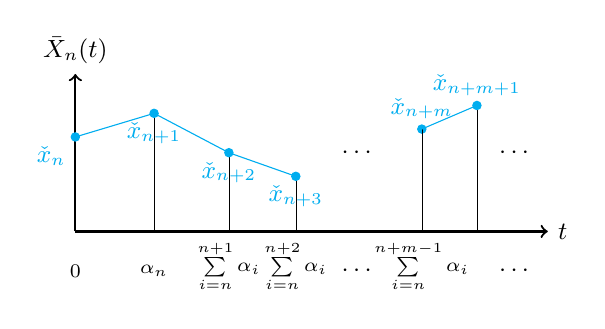
\begin{tikzpicture}
	\draw[->,thick] (0,0) -- (6,0) node[right] {\small $t$};
	\draw[->,thick] (0,0) -- (0,2) node[above] {\small $\bar{X}_{n}(t)$};
	
	\coordinate (x0) at (0, 1.2);
	\node (0) at (0, -0.5) { \scriptsize $0$};
	\coordinate (x1) at (1.0, 1.5);
	\coordinate (t1) at (1.0, 0);
	\node (alphan) at (1.0, -0.5) { \scriptsize $\alpha_{n}$};
	\coordinate (x2) at (1.95, 1.0);
	\coordinate (t2) at (1.95, 0);
	\coordinate (x3) at (2.8, 0.7);
	\coordinate (t3) at (2.8, 0);
	\node (dotsx) at (3.6, 1.0) {\small $\cdots$};
	\node (dotst) at (3.6, -0.5) {\small $\cdots$};
	\coordinate (xm) at (4.4, 1.3);
	\coordinate (tm) at (4.4, 0);
	\coordinate (xm1) at (5.1, 1.6);
	\coordinate (tm1) at (5.1, 0);
	\coordinate (xm2) at (5.75, 0.8);
	\coordinate (tm2) at (5.75, 0);
	\node (dotsx2) at (5.6, 1.0) {\small $\cdots$};
	\node (dotst2) at (5.6, -0.5) {\small $\cdots$};
	
	
	\filldraw [cyan] (x0) circle (1.5pt) node[below left] {\small $\xcheck_{n}$};
	
	\draw[very thin] (x1) -- (t1); 
	%			node[below] {\small $\alpha_{n}$};
	\draw[-, cyan] (x0) -- (x1);
	\filldraw[cyan] (x1) circle (1.5pt) node[below] {\small $\check{x}_{n+1}$};
	
	\draw[very thin] (x2) -- (t2) node[below] {\scriptsize $\sum\limits_{i=n}^{n+1}\alpha_{i}$};
	\draw[-, cyan] (x1) -- (x2);
	\filldraw[cyan] (x2) circle (1.5pt) node[below] {\small $\check{x}_{n+2}$};
	
	\draw[very thin] (x3) -- (t3) node[below] {\scriptsize $\sum\limits_{i=n}^{n+2}\alpha_{i}$};
	\draw[-, cyan] (x2) -- (x3);
	\filldraw[cyan] (x3) circle (1.5pt) node[below] {\small $\check{x}_{n+3}$};
	
	\filldraw [cyan] (xm) circle (1.5pt) node[above] {\small $\xcheck_{n+m}$};
	\draw[very thin] (xm) -- (tm) node[below] {\scriptsize $\sum\limits_{i=n}^{n+m-1}\alpha_{i}$};
	
	\draw[very thin] (xm1) -- (tm1); 
	%			node[below] {\scriptsize $\sum\limits_{i=n}^{n+m}\alpha_{i}$};
	\draw[-, cyan] (xm) -- (xm1);
	\filldraw[cyan] (xm1) circle (1.5pt)
	node[above] {\small $\check{x}_{n+m+1}$};
	
	%		\draw[very thin] (xm2) -- (tm2); 
	%		\draw[-, cyan] (xm1) -- (xm2);
	%		\filldraw[cyan] (xm2) circle (1.5pt) node[below] {\small $\check{x}_{n+m+2}$};
	
\end{tikzpicture}
%		\caption{}
%		\label{fig:image1}
	\end{minipage}
	\hspace{0.05\textwidth} 
	\begin{minipage}[b]{0.45\textwidth}
		\centering
	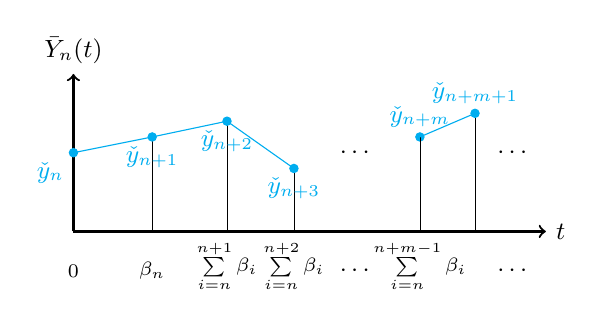
\begin{tikzpicture}
	\draw[->,thick] (0,0) -- (6,0) node[right] {\small $t$};
	\draw[->,thick] (0,0) -- (0,2) node[above] {\small $\bar{Y}_{n}(t)$};
	
	\coordinate (x0) at (0, 1.0);
	\node (0) at (0, -0.5) { \scriptsize $0$};
	\coordinate (x1) at (1.0, 1.2);
	\coordinate (t1) at (1.0, 0);
	\node (alphan) at (1.0, -0.5) { \scriptsize $\beta_{n}$};
	\coordinate (x2) at (1.95, 1.4);
	\coordinate (t2) at (1.95, 0);
	\coordinate (x3) at (2.8, 0.8);
	\coordinate (t3) at (2.8, 0);
	\node (dotsx) at (3.6, 1.0) {\small $\cdots$};
	\node (dotst) at (3.6, -0.5) {\small $\cdots$};
	\coordinate (xm) at (4.4, 1.2);
	\coordinate (tm) at (4.4, 0);
	\coordinate (xm1) at (5.1, 1.5);
	\coordinate (tm1) at (5.1, 0);
	\coordinate (xm2) at (5.75, 0.9);
	\coordinate (tm2) at (5.75, 0);
	\node (dotsx2) at (5.6, 1.0) {\small $\cdots$};
	\node (dotst2) at (5.6, -0.5) {\small $\cdots$};
	
	
	\filldraw [cyan] (x0) circle (1.5pt) node[below left] {\small $\ycheck_{n}$};
	
	\draw[very thin] (x1) -- (t1); 
	%			node[below] {\small $\alpha_{n}$};
	\draw[-, cyan] (x0) -- (x1);
	\filldraw[cyan] (x1) circle (1.5pt) node[below] {\small $\check{y}_{n+1}$};
	
	\draw[very thin] (x2) -- (t2) node[below] {\scriptsize $\sum\limits_{i=n}^{n+1}\beta_{i}$};
	\draw[-, cyan] (x1) -- (x2);
	\filldraw[cyan] (x2) circle (1.5pt) node[below] {\small $\check{y}_{n+2}$};
	
	\draw[very thin] (x3) -- (t3) node[below] {\scriptsize $\sum\limits_{i=n}^{n+2}\beta_{i}$};
	\draw[-, cyan] (x2) -- (x3);
	\filldraw[cyan] (x3) circle (1.5pt) node[below] {\small $\check{y}_{n+3}$};
	
	\filldraw [cyan] (xm) circle (1.5pt) node[above] {\small $\ycheck_{n+m}$};
	\draw[very thin] (xm) -- (tm) node[below] {\scriptsize $\sum\limits_{i=n}^{n+m-1}\beta_{i}$};
	
	\draw[very thin] (xm1) -- (tm1); 
	%			node[below] {\scriptsize $\sum\limits_{i=n}^{n+m}\alpha_{i}$};
	\draw[-, cyan] (xm) -- (xm1);
	\filldraw[cyan] (xm1) circle (1.5pt)
	node[above] {\small $\check{y}_{n+m+1}$};
	
	%		\draw[very thin] (xm2) -- (tm2); 
	%		\draw[-, cyan] (xm1) -- (xm2);
	%		\filldraw[cyan] (xm2) circle (1.5pt) node[below] {\small $\check{z}_{n+m+2}$};
\end{tikzpicture}
%		\caption{}
%		\label{fig:image2}
	\end{minipage}
	\caption{Construction of $\xbar_{n}(\cdot)$ and $\ybar_{n}(\cdot)$}
	\label{fig:xybar}
\end{figure}


\subsection{Decoupled Functional Central Limit Theorems}

%\subsection{Step~3: Derive the Decoupled Functional Central Limit Theorem}
\label{sec:fclt:theo}

With $\{ \xbar_{n}(\cdot) \}_{n=1}^\infty$ and $\{ \ybar_{n}(\cdot) \}_{n=1}^\infty$ defined in \eqref{eq:xbar-short} and \eqref{eq:ybar-short}, we could establish the following decoupled FCLT.

\begin{thm}[Decoupled functional central limit theorems]\label{thm:fclt-twotime}
	Suppose that Assumptions~\ref{assump:smooth} -- \ref{assump:noise-fclt} and \ref{assump:mart-decouple-rate} hold.
	\begin{enumerate}[(i)]
		\item \label{thm:fclt-x} The stochastic process $\xbar_{n}(\cdot)$ defined in \eqref{eq:xbar-short} converges weakly to the stationary solution of the following SDE 
		\begin{equation}\label{eq:fclt-twotime:x-sde}
			d \ermX(t) = - B_1 \ermX(t) dt + \Sigma_{\xi}^{1/2} d \ermW^{d_x}(t).
		\end{equation}
		The rescaled iterate $ \xcheck_{n} $ defined in \eqref{eq:xycheck-def} converges weakly to the invariant distribution of \eqref{eq:fclt-twotime:x-sde}, i.e., $\NM(0, \Sigma_x)$, where $\Sigma_x$ satisfies the following Lyapunov equation 
		\begin{equation}\label{eq:fclt-twotime:x-var}
			B_1 \Sigma_x + \Sigma_x B_1 = \Sigma_{\xi}.
		\end{equation}
%		\item The stochastic process $\zbar_{n}(\cdot)$ defined in \eqref{eq:def:zbar} converges weakly to the stationary solution of the following SDE
%		\begin{align}\label{eq:fclt-twotime:y-sde}
%			d \ermY(t) = - \left(B_3 - \frac{\invdiffslow \mI}{2}  \right) \ermY(t) dt + \widetilde{\Sigma}_{\psi}^{1/2} d \ermW^{d_y}(t),
%		\end{align}
%		where $\widetilde{\Sigma}_{\psi}$ is defined in \eqref{eq:cov-z}.
		\item \label{thm:fclt-y} The stochastic process $\ybar_{n}(\cdot)$ defined in \eqref{eq:ybar-short} converges weakly to the stationary solution of the following SDE 
		\begin{equation}\label{eq:fclt-twotime:y-sde}
			d \ermY(t) = - \left(B_3 - \frac{\invdiffslow \mI}{2}  \right) \ermY(t) dt + \widetilde{\Sigma}_{\psi}^{1/2} d \ermW^{d_y}(t),
		\end{equation}
		where the matrix $\widetilde{\Sigma}_{\psi}$ is defined as 
		\begin{equation}\label{eq:cov-z}
			\widetilde{\Sigma}_{\psi} := \Sigma_{\psi} - B_2 B_1^{-1} \Sigma_{\xi,\psi} - \Sigma_{\xi, \psi}^\top B_1^{-\top} B_2^\top + B_2 B_1^{-1} \Sigma_{\xi} B_1^{-\top} B_2^\top.
		\end{equation}
		The rescaled iterate $ \ycheck_{n}$ defined in \eqref{eq:xycheck-def} converges weakly to the invariant distribution of \eqref{eq:fclt-twotime:y-sde}, i.e., $\NM(0, \Sigma_y)$, where $\Sigma_y$ satisfies the following Lyapunov equation
		\begin{equation}\label{eq:fclt-twotime:y-var}
			\left(B_3 - \frac{\invdiffslow \mI}{2} \right) \Sigma_y + \Sigma_y \left( B_3 - \frac{\invdiffslow \mI}{2} \right) = \widetilde{\Sigma}_{\psi}.
		\end{equation}
	\end{enumerate}
\end{thm}

\begin{rema}[Explanation of Theorem~\ref{thm:fclt-twotime}]\label{rema:fclt}
	For Theorem~\ref{thm:fclt-twotime}, we have the following explanations.
	\begin{enumerate}[(i)]
		\item \textbf{Ornstein-Uhlenbeck process}: 
		The drift terms in the SDEs \eqref{eq:fclt-twotime:x-sde} and \eqref{eq:fclt-twotime:y-sde} are linear, and the noise terms are constant. 
		As a result, the solution to these SDEs is a multi-dimensional Ornstein-Uhlenbeck process. Assumption~\ref{assump:hurwitz} ensures the uniqueness of the invariant distribution for these processes, with covariance matrices given in \eqref{eq:fclt-twotime:x-var} and \eqref{eq:fclt-twotime:y-var}~\citep[Section~6.5]{risken1996fokker}.
		
		\item \textbf{Stationary solution}:
		A ``stationary solution'' refers to a solution that is a stationary process. Specifically, this corresponds to a solution where the initial distribution matches the invariant distribution.
		
		\item \textbf{Interdependence}: The parameters $B_1$ and $\Sigma_{\xi}$ in \eqref{eq:fclt-twotime:x-sde} are associated solely with the fast-time-scale updates, indicating that the asymptotic behavior of the fast iterate resembles standard SA and is nearly unaffected by the slow iterate.
		In contrast, both $B_3$ and $\widetilde{\Sigma}_{\psi}$ in \eqref{eq:fclt-twotime:y-sde} are influenced by the slow-time-scale update.
		Specifically, $B_3$ (as detailed in Remark~\ref{remar:fclt:B-form}) involves the gradient of $F$, and $\widetilde{\Sigma}_{\psi}$ represents the asymptotic covariance of $\psi_{n} - B_2 B_1^{-1} \xi_{n}$.
		Decoupling ensures that the convergence rates of different iterates depend only on their respective step sizes. However, the fast-time-scale update still influences the slow-time-scale update through the constant terms, such as the coefficients in \eqref{eq:fclt-twotime:y-sde}.
		
		\item \textbf{Effect of step sizes}: The presence of $\invdiffslow$ in \eqref{eq:fclt-twotime:y-sde} highlights the impact of step sizes on asymptotic behavior. As illustrated in Example~\ref{exmp:fclt-stepsize}, for $\beta_{n} = \Theta(n^{-b})$ with $b \in (0,1]$, $\invdiffslow = \beta_{0}^{-1} \neq 0$ only when $b=1$, which requires the initial step size to be sufficiently large. This aligns with the convergence analysis for standard SA~\citep{moulines2011non}.
		Due to the assumption $\beta_{n} / \alpha_{n} = o(1)$, the choice of step sizes does not influence the asymptotic behavior in \eqref{eq:fclt-twotime:x-sde} (see Remark~\ref{rema:step-size}).
	\end{enumerate}
\end{rema}



\begin{rema}[Comparison with previous work]
%	\begin{enumerate}[(i)]
%		\item Our FCLTs could recover the classical CLTs in \cite{konda2004convergence, mokkadem2006convergence}, as shown in Corollary~\ref{cor:clt}.
%		\item 
Compared to the FCLT presented in~\cite{faizal2023functional}, which rescales the error terms $\xhat_{n}$ and $\yhat_{n}$ using the square root of the fast-time-scale step size, we apply distinct rescalings to $\xhat_{n}$ and $\yhat_{n}$ based on the square root of their respective step sizes.
This refinement enables us to derive decoupled FCLTs under local linearity conditions, offering a more precise characterization of the asymptotic behavior in two-time-scale SA. Furthermore, our FCLTs can recover the classical CLTs from \cite{konda2004convergence, mokkadem2006convergence}, as demonstrated in Corollary~\ref{cor:clt}.
\end{rema}

\begin{cor}[Central limit theorems]\label{cor:clt}
	Under the conditions of Theorem~\ref{thm:fclt-twotime}, we have 
	$\alpha_{n}^{-1/2} (\xx_{n} - H(\yy_{n})) \weakconverge \NM(0, \Sigma_x)$, 
	$ \beta_{n}^{-1/2} (\yy_{n} - \yy^\star) \weakconverge \NM(0,\Sigma_{y})$ and
	$ \alpha_{n}^{-1/2} (\xx_{n} - \xx^\star) \weakconverge \NM(0, \Sigma_{x})$.
\end{cor}


\subsection{Examples}
\label{sec:fclt:exam}

In this subsection, we present several examples of two-time-scale SA and demonstrate the application of our FCLTs to these cases. To simplify the discussion, we assume the required conditions are satisfied, bypassing the detailed verification processes. Our focus is primarily on the drift and diffusion terms in \eqref{eq:fclt-twotime:x-sde} and \eqref{eq:fclt-twotime:y-sde}.

In the following two examples, we consider the problem of minimizing a strongly convex function $f$ with a unique minimizer $x_o^\star = \arg\min_{x} f(x)$, using noisy gradient observations.
%When $f$ has continuous Hessian, Assumptions~\ref{assump:smooth} to \ref{assump:near-linear} hold.


\begin{exam}[SGD with Polyak-Ruppert averaging]\label{exmp:PRave}
	Stochastic gradient descent (SGD), introduced by \citep{robbins1951stochastic}, iteratively updates the iterate $x_t$ by~\eqref{eq:SGD}.
	To improve the convergence of SGD, an additional averaging step~\eqref{eq:SGD-averaging} is often used~\citep{polyak1992acceleration,ruppert1988efficient}
	%	Suppose that we want to minimize a function $f$ satisfying Assumption~\ref{assump:example}\ref{assump:example1} with access only to the noisy observations of the true gradients.
	%	% As analyzed in Section~\ref{sec:intro},
	%	To find the true minimizer $x_o^{\star}$, 
	%	% SGD with Polyak-Rupert averaging~\eqref{eq:SGD-both} \citep{polyak1992acceleration,ruppert1988efficient}
	%	the stochastic gradient method (SGD)~\citep{robbins1951stochastic} iteratively updates the iterate $x_t$ by~\eqref{eq:SGD}.
	%	In order to improve the convergence of SGD, an additional averaging step~\eqref{eq:SGD-averaging} is often used~\citep{polyak1992acceleration,ruppert1988efficient}
	%	To minimize a strongly function $f$ with minimizer $x^\star = \arg\min_{x} f(x)$, the update rule of SGD with 
	\begin{subequations} \label{eq:SGD-both}
		\begin{align}
			x_{n+1} &= x_{n} - \alpha_n(\nabla f(x_{n}) + \xi_{n})~\text{with}~\alpha_n = \frac{\alpha_0}{ (n+1)^a }~(0 < a < 1)  \label{eq:SGD}, \\
			y_{n+1} &= \frac{1}{n+1}\sum_{\tau=0}^n x_{\tau} = y_n - \beta_n(y_n-x_n)~\text{with}~\beta_n = \frac{1}{n+1}. \label{eq:SGD-averaging}
		\end{align}
	\end{subequations}
	This update is a special case 
	of \eqref{alg:xy} with $F(x, y) = \nabla f(x)$, $G(x, y) = y -x$, $H(y) \equiv x^{\star}$ and $y^{\star} 
%	= x^{\star} 
	= x_o^{\star}$.
	%	It follows that $G(H(y), y) = y - x^\star$ and $y^{\star} = x^{\star} = x_o^{\star}$.
	%	One can check that
	%	Assumptions \ref{assump:smooth:FH}  -- \ref{assump:near-linear} hold with $L_H=S_H= \SBG =0$,  $L_F =  L$, $\mu_F= \mu$,  $\LGx = \LGy = \mu_G = 1$, $\SBF=S$ and $\Fsmooth=1$.
	%	Now we contextualize this example within the framework of \eqref{eq:two-loop-approx}.
	%	In the inner loop, our goal is to reduce the norm of $\nabla f(x)$, while in the outer loop, we strive to approach $x_o^\star$.
	%	Under Assumption~\ref{assump:example}\ref{assump:example1}, the two objectives coincide.
	%	\citet{moulines2011non} have demonstrated that $\EB \| x_t - x^\star \|^2 = \OM(\alpha_t)$ and $\EB\| y_t - y^\star \|^2 = \OM (1/t)$ as long as $a \ge 1/2$.
	%	Given the improved convergence rate of the averaged sequence, our primary interest lies in the slow iterate $y_t$.
	%With $F(x,y) = \nabla f(x^\star)$ and $G(x,y) = y-x$. $H(y) \equiv x^{\star}$. $\xhat_{n} = x_n - x^\star$ and $\yhat_{n} = y_n - y^\star$.
	Contextualizing in Theorem~\ref{thm:fclt-twotime}, one can check 
	$B_1 = \nabla^2 f(x)$, $B_3 - \frac{\invdiffslow }{2} \mI =  \frac{1}{2} \mI $ and $\widetilde{\Sigma}_\psi = [ \nabla^2 f(x_o^\star) ]^{-1} \Sigma_{\xi} [ \nabla^2 f(x_o^\star) ]^{-1} $.
	Thus, the solution to \eqref{eq:fclt-twotime:y-var} is $\Sigma_{y} = \widetilde{\Sigma}_{\psi}$.
	We recover the CLT for the averaged iterate from \cite{polyak1992acceleration} and the FCLT for the original iterate from \cite[Section~II.4.5.3]{benveniste2012adaptive} and \cite[Section~8.4]{borkar2009stochastic}. Additionally, our results offer a trajectory-level characterization for the averaged iterate.
\end{exam}

\begin{exam}[SGD with momentum]\label{exmp:momentum}
	Stochastic heavy ball (SHB) is a variant of SGD based on momentum and adaptive step sizes and has been shown to be effective~\citep{gadat2018stochastic}.
	A ``normalized''  version of SHB~\citep{gupal1972stochastic,gitman2019understanding} iteratively runs
	\begin{equation}\label{eq:SHB}
		\begin{aligned}
			x_{n+1} &= x_{n} - \alpha_n (x_n - \nabla f(y_n) - \xi_n),\\
			y_{n+1} &= y_{n} - \beta_n  x_{n}.
		\end{aligned}
	\end{equation}
	%	Here one should interpret $x_{t}$ as a (stochastic) search direction that is defined to be a combination of the current stochastic gradient $\nabla f(y_t) + \xi_t$
	%	and past search direction $x_t$.\footnote{Here we employ a slightly different update rule for $y_t$ to be consistent with~\citet{doan2022nonlinear}. 
		% The original update rule is $y_{t+1} = y_{t} - \beta_t  x_{t+1}$ in these papers. We do not use the updated $x_{t+1}$ to update $y_{t+1}$ for the consistency with~\citep{doan2022nonlinear}. 
		%		As analyzed in Appendix~\ref{sec:discuss:alter},
		% Remark~\ref{rema:momentum-another}, 
		%		this modification makes no difference in terms of convergence rates.}
	%	Under Assumption~\ref{assump:example}, these two updates are 
	This update is a special case of 
	%	the nonlinear two-time-scale SA in 
	\eqref{alg:xy} with $F(x, y) = x-\nabla f(y), G(x, y) = x$, $H(y) = \nabla f(y)$,
	%	It follows that $G(H(y), y) = \nabla f(y)$,
	$y^{\star} = x_o^{\star}$ and $x^{\star} = 0$.
	%	One can check that Assumptions \ref{assump:smooth:FH}  -- \ref{assump:near-linear} hold with $L_H = \LGy = L$, $L_F = \LGx = 1$, $\mu_F= 1$, $\mu_G = \mu$, $\Hsmooth=1$, $S_H = S/2$, $\SBF=0$, $\SBG=S$ and $\Gsmooth=1$.
	%	
	%	Now, we integrate this example into the framework of \eqref{eq:two-loop-approx}.
	%	In the inner loop, our objective is to approximate the gradient of a fixed $y$, while 
	%	% where the inner-loop residual $x_t - H(y_t)$ signifies the distinction between the search direction $x_t$ and the gradient $\nabla g(y_t)$ at the current point $y_t$.
	%	in the outer loop, we aim to locate the stationary point (also the minimizer) $x_o^\star$, 
	%	% and the outer-loop residual represents the difference between the current point $y_t$ and the solution $x^o_\star$.
	%	Thus, our primary focus lies in the slow iterate $y_t$.
	%	
	%	% In this example, a seemingly peculiar phenomenon is that $G(x,y)$ is independent of $y$.
	%	% In fact, after setting $x = H(y)$,
	%	% $G(H(y), y)$ is the gradient of the objective function,
	%	% an operator with a more precise meaning.
	%	% Moreover, Assumptions~\ref{assump:G} and \ref{assump:sm:F} also imply that
	%	% $G(H(y), y)$ would play a more important role than $G(x,y)$ in our theoretical analysis.
	%	% For instance, in our assumptions, only \eqref{assump:G:smooth} is solely related to $G(x,y)$, while \eqref{assump:G:smooth2} and \eqref{assump:G:sm} are both on $G(H(y), y)$.
	Contextualizing this example in Theorem~\ref{thm:fclt-twotime}, one can check
	$B_1 = \mI$, $B_3 - \frac{\invdiffslow}{2} \mI = \nabla^2 f(x^\star) - \frac{\invdiffslow}{2} \mI$ and $\widetilde{\Sigma}_{\psi} = \Sigma_{\xi}$, 
	implying that the asymptotic behavior is similar to that of standard SA.
	Consequently, for a strongly convex objective, the addition of momentum does not provide an asymptotic advantage over SGD. Furthermore, our result is not directly comparable to the FCLT in \cite{gadat2018stochastic}, as we consider distinct time scales, whereas their analysis focuses on a single-time-scale setting.
\end{exam}

In the two examples above, while the update for the slow iterate $y_{n}$ is deterministic, the limiting trajectories remain stochastic, capturing the influence of the fast-time-scale updates on the slow-time-scale dynamics.

\begin{exam}[Gradient-based temporal-difference learning]\label{exmp:gtd}
	Gradient-based temporal-difference (TD) algorithms are widely used in off-policy reinforcement learning (RL), such as policy evaluation with function approximation~\citep{sutton2008convergent, sutton2009fast, maei2009convergent}.
	We consider two specific algorithms: GTD2 and TDC with linear function approximation~\citep{sutton2009fast}. These algorithms serve as typical examples of two-time-scale SA~\citep{dalal2018finite}. For clarity, we concentrate on the specific update rules while omitting the details of the RL setup. A more comprehensive explanation is provided in Appendix~\ref{append:exmp}.

	In this problem, the goal is to estimate the value function $V(s)$ for a given policy using a linear parameterization $V(s; y) = \phi(s)^\top y$, where $\phi(s)$ represents the feature vector of state $s$, and $y$ denotes the parameter vector.
	Given i.i.d.\ samples $\{ (s_n, r_n, s'_n) \}_{n=0}^\infty$~\citep{sutton2008convergent}, where $s_n$ is the current state, $r_n$ is the reward and $s'_n$ is the next state, the optimal parameter $y$ can be estimated iteratively via the following update rules\footnote{
	Compared to the original formulation in \cite{sutton2009fast}, we incorporate an importance weight $\rho_{n}$, the explicit form of which is provided in Appendix~\ref{append:exmp}.}
	\begin{align}
		x_{n+1} &= x_{n} - \alpha_{n} \big( \phi(s_{n})^{\top} x_{n} - \rho_{n} \delta_{n} \big) \phi(s_{n}), \label{eq:gtd-x}\\
		y_{n+1} &= y_{n} - \beta_{n} \rho_{n} \big( \gamma \phi(s'_{n}) - \phi(s_{n}) \big) \phi(s_{n})^\top x_{n}, \label{eq:gtd2-y}\  \qquad \mathrm{ (GTD2) }   \\
		y_{n+1} &= y_{n} - \beta_{n} \rho_{n} \big( \gamma \phi(s'_n) \phi(s_n)^\top x_{n} - \delta_{n} \phi(s_{n}) \big), \label{eq:tdc-y} \ \quad \,  \mathrm{ (TDC) }
	\end{align}
	where $\gamma$ is the discount factor, $\rho_{n}$ is the importance weight, and $\delta_{n}$ is the temporal-difference error defined as $	\delta_{n} = r_{n} + ( \gamma \phi(s'_{n}) - \phi(s_n) )^\top y_{n} $.
	Here, the fast iterate $x_{n}$ is an auxiliary variable.
	Both GTD2 and TDC share the same fast time-scale update but differ in their slow time-scale updates.
	
	To contextualize these methods within the two-time-scale SA~\eqref{alg:xy}, we define $A_n =  \rho_{n} \phi(s_n) ( \phi(s_n) - \gamma \phi(s'_n) )^\top $, $b_n = \rho_{n} r_{n} \phi(s_n) $, $C_n = \phi(s_{n}) \phi(s_n)^\top $, $D_n = \gamma \rho_{n} \phi(s_n) \phi(s'_n)^\top$, and their expectations $A= \EB[A_n]$, $b = \EB[b_n]$, $C=\EB[C_n]$, and $D=\EB[D_n]$.
	It can be checked that \eqref{eq:gtd-x} -- \eqref{eq:tdc-y} are an instance of \eqref{alg:xy} with
	\begin{equation*}
		F(x,y) = Cx +Ay-b,\ \ 
		\Ga(x,y) = -A^\top x,\ \ 
		\Gb (x,y) = D^\top x + Ay - b.
	\end{equation*}
%	Then we can check $F(x,y) = Cx +Ay-b $, 
%	$\Ga(x,y) = -A^\top x$, and $ \Gb (x,y) = D^\top x + Ay - b$.
	It follows that $H(y) = -C^{-1}(Ay-b)$, implying
	$\Ga(H(y), y) = A^\top C^{-1} (Ay- b)$ and $\Gb(H(y), y) = (C - D^\top) C^{-1} (Ay - b)$.
	Although these expressions appear different, it can be verified that $C - D^\top = A^\top$ \citep[Equation~(68)]{li2024high}, leading to $\Ga (H(y), y) \equiv \Gb(H(y),y)$. 
	Therefore, GTD2 and TDC have the same optimal solution, $y^\star = A^{-1} b$ and $x^\star = H(y^\star) = 0$. Furthermore, the drift terms for both the methods in \eqref{eq:fclt-twotime:x-sde} and \eqref{eq:fclt-twotime:y-sde} are identical: $B_1 = C$ and $B_3 = A^\top C^{-1} A$.
	
	For the noise terms, both the methods share the same noise for the fast time scale $\xi_{n} = C_n x_{n} + A_n y_n - b_n - F(x_n, y_n) $.
	On the slow time scale, however, the noise differs slightly. For GTD2, the noise is expressed as $\psia_{n} = - A_{n}^\top x_n - \Ga(x_n, y_n) $, whereas for TDC, it is given by $\psib_{n} = D_n^\top x_{n} + A_n y_n - b_n - \Gb(x_n, y_n)$.
	Despite these differences, both the methods ultimately result in the same diffusion term $\widetilde{\Sigma}_{\psi}$ in \eqref{eq:fclt-twotime:y-sde}. Additional details can be found in Appendix~\ref{append:exmp}.
	
	In summary, while GTD2 and TDC differ in form and may display distinct numerical behaviors~\citep{dann2014policy}, they share identical asymptotic properties, aligning with the results of~\citep{hu2024central}. Compared to their work, our results provide a more detailed characterization of trajectory properties for i.i.d.\ samples.
\end{exam}



\section{Framework of Proof}
\label{sec:fclt:proof-frame}

In this section, we outline the framework of the proof, which is divided into four key steps: (i) deriving the one-step recursion; (ii) establishing the tightness of the sequences constructed in Section~\ref{sec:fclt:construct}; (iii) demonstrating that these sequences approximately solve the corresponding martingale problems; and (iv) combining the results from the previous steps to derive the decoupled FCLT.
The main content for these steps is detailed in Sections~\ref{sec:fclt:one-step} -- \ref{sec:fclt:intergrate}. 

Notably, in Section~\ref{sec:fclt:one-step}, we introduce an auxiliary sequence $\{ \zcheck_{n} \}_{n=1}^\infty$ and construct the associated continuous-time trajectories $\{ \zbar_{n}(\cdot) \}_{n=1}^\infty$. The introduction of this auxiliary sequence represents one of the primary novelties of our work and serves as a cornerstone of the proof. \Figref{fig:proof-sketch} offers a visual summary of the proof framework. The blue, green, yellow, and white blocks correspond to the four steps outlined above, providing a clear and intuitive depiction of the overall structure.


\begin{figure}[t]\centering
	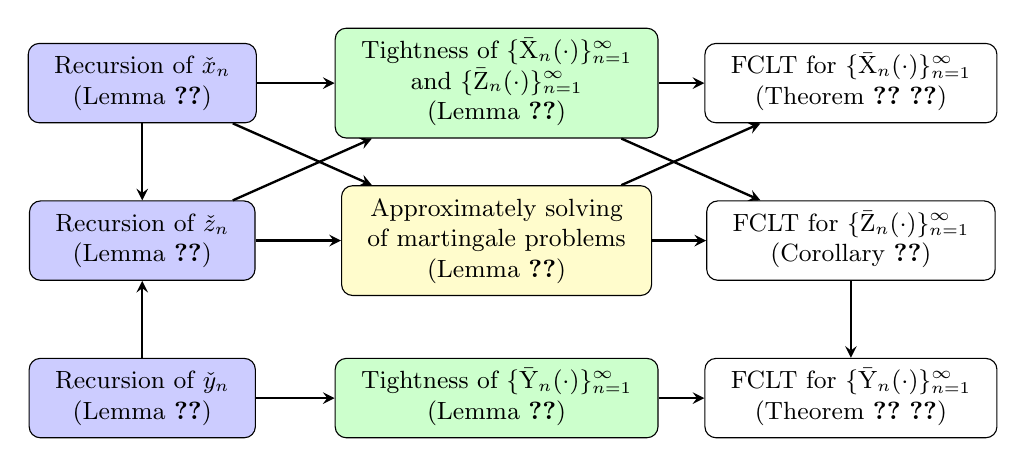
\begin{tikzpicture}[>=stealth,every node/.style={shape=rectangle,draw,rounded corners, minimum width=1cm, node distance=0.8cm},]
				
		\node[fill=blue!20] (xcheck) at (-4.5,2) {\small \begin{tabular}{c}
				Recursion of $\xcheck_{n}$ \\
				(Lemma~\ref{lem:check-twotime-xy})
			\end{tabular} };
		\node[fill=blue!20] (zcheck) at (-4.5,0) 
		{\small \begin{tabular}{c}
				Recursion of $\zcheck_{n}$ \\
				(Lemma~\ref{lem:check-twotime-z})
			\end{tabular} };
		\node[fill=blue!20] (ycheck) at (-4.5,-2)
		{\small \begin{tabular}{c}
				Recursion of $\ycheck_{n}$ \\
				(Lemma~\ref{lem:check-twotime-xy})
			\end{tabular} };
		
		\draw[->, line width=.3mm] (xcheck) to (zcheck);
		\draw[->, line width=.3mm] (ycheck) to (zcheck);
		
		\node[fill=yellow!20] (martprob) at (0,0)
		{\small \begin{tabular}{c}
				Approximately solving \\ 
				of martingale problems \\
				(Lemma~\ref{lem:mart-prob-twotime})
		\end{tabular} };
		\node[fill=green!20] (xztight) at (0,2)
		{\small \begin{tabular}{c}
				Tightness of $\{ \xbar_{n}(\cdot) \}_{n=1}^\infty$ \\
				 and $\{ \zbar_{n}(\cdot) \}_{n=1}^\infty$ \\
				(Lemma~\ref{lem:tight-twotime})
			\end{tabular}};
		
		\node[fill=green!20] (ytight) at (0,-2)
		{\small \begin{tabular}{c}
				Tightness of $\{ \ybar_{n}(\cdot) \}_{n=1}^\infty$ \\
				(Lemma~\ref{lem:tight-twotime})
			\end{tabular} };
		
		\draw[->, line width=.3mm] (xcheck) to  (xztight);
		\draw[->, line width=.3mm] (zcheck) to  (xztight);
		\draw[->, line width=.3mm] (xcheck) to (martprob);
		\draw[->, line width=.3mm] (zcheck) to (martprob);
		\draw[->, line width=.3mm] (ycheck) to (ytight);
		
		\node (zfclt) at (4.5, 0)
		{\small \begin{tabular}{c}
				FCLT for $\{ \zbar_{n}(\cdot) \}_{n=1}^\infty$ \\
				(Corollary~\ref{cor:fclt-z})
		\end{tabular}  };
		\node (xfclt) at (4.5,2)
		{\small \begin{tabular}{c}
				FCLT for $\{ \xbar_{n}(\cdot) \}_{n=1}^\infty$ \\
				(Theorem~\ref{thm:fclt-twotime}~\ref{thm:fclt-x})
			\end{tabular}  };
		\node (yfclt) at (4.5, -2)
		{\small \begin{tabular}{c}
				 FCLT for $\{ \ybar_{n}(\cdot) \}_{n=1}^\infty$ \\
				 (Theorem~\ref{thm:fclt-twotime}~\ref{thm:fclt-y})
			\end{tabular}};
		
		\draw[->, line width=.3mm] (xztight) to (xfclt);
		\draw[->, line width=.3mm] (xztight) to (zfclt);
		\draw[->, line width=.3mm] (martprob) to (xfclt);
		\draw[->, line width=.3mm] (martprob) to (zfclt);
		\draw[->, line width=.3mm] (ytight) to (yfclt);
		\draw[->, line width=.3mm] (zfclt) to (yfclt);
	\end{tikzpicture}
	\caption{Illustration for the framework of proof.}
	\label{fig:proof-sketch}
\end{figure}



\subsection{Derivation of One-Step Recursions and Introduction of the Auxiliary Sequence}
\label{sec:fclt:one-step}

With the rescaled sequence defined in \eqref{eq:xycheck-def}, we derive their one-step recursion formulas as follows.

\begin{lem}[One-step recursions for $\xcheck_{n}$ and $\ycheck_{n}$]\label{lem:check-twotime-xy}
	Suppose that Assumptions~\ref{assump:smooth} -- \ref{assump:stepsize-twotime} and \ref{assump:mart-decouple-rate} hold.
	Define $\tilde{\xi}_{n} := \xi_{n} - \kappa_{n} H^\star \psi_{n}$. 
%	and $\tilde{\psi}_{n} := \psi_{n} - B_2 B_1^{-1} \tilde{\xi}_n$. 
	The rescaled sequences $\{ \xcheck_{n} \}_{n=0}^\infty$ and $\{ \ycheck_{n} \}_{n=0}^\infty$ defined in \eqref{eq:xycheck-def} 
	satisfy the following relationships  
	\begin{align}
		\xcheck_{n+1} & = (\mI - \alpha_{n} B_1) \xcheck_{n} - \sqrt{\alpha_{n}} \tilde{\xi}_{n} + R_{n}^x, \label{eq:xcheck-twotime} \\
		\ycheck_{n+1}
		& = \left( \mI - \beta_{n} B_3 + \frac{ \invdiffslow \beta_{n} }{2} \mI \right) \ycheck_{n} - \sqrt{\beta_{n} \alpha_{n} } B_2 \xcheck_{n} - \sqrt{\beta_n} \psi_{n} + R_{n}^y. \label{eq:ycheck-twotime}
%		\zcheck_{n+1} & = \left( \mI - \beta_{n} B_3 + \frac{\invdiffslow \beta_{n}}{2} \mI \right) \zcheck_{n} - \sqrt{\beta_{n}} \tilde{\psi}_{n} + R_{n}^z. \label{eq:zcheck-twotime}
	\end{align}
	For any $2 < p \le \frac{4}{1 + ( \Hsmooth \vee \Fsmooth \vee \Gsmooth )/2} $, 
	the residual terms $R_{n}^x$ and $R_{n}^y$ 
%	and $R_{n}^z$ 
	have the following properties:
%	\begin{enumerate}[(i)]
%		\item 
		(i) $\EB \| \EB [ R_{n}^x | \FM_n ] \| = o(\sqrt{\beta_{n} \alpha_{n}}) $, $\EB \| R_{n}^x \|^2 = \OM(\beta_{n} \alpha_{n})$ and $\EB \| R_{n}^x \|^p = o(\alpha_{n})$;
%		\item 
		(ii) $\EB \| R_{n}^y \|^2 = o(\beta_{n}^2)$ and $\EB \| R_{n}^y \|^p = o(\beta_{n})$.
%		\item $\EB \| \EB [ R_{n}^z | \FM_n ] \| = o(\beta_{n} ) $, $\EB \| R_{n}^z \|^2 = \OM(\beta_{n}^2 )$ and $\EB \| R_{n}^z \|^p = o(\beta_{n})$.
%	\end{enumerate}
\end{lem}

Under the local linearity assumption, $\xcheck_{n+1}$ can be decomposed into three components: a linear transformation of the previous iterate $\xcheck_{n}$,
a noise term $\sqrt{\alpha_{n}} \tilde{\xi}_{n}$ and a high-order residual term $R_n^x$.
The influence of $\ycheck_{n}$ on \eqref{eq:xcheck-twotime} is negligible for two reasons: (i) the noise term is adjusted to $\tilde{\xi}_{n}$, where $\tilde{\xi}_{n} = \xi_{n} + o_p(1)$; (ii) the residual term $R_n^x$ is asymptotically negligible.
As a result, the behavior of the sequence $\{ 
\xcheck_{n} \}_{n=0}^\infty$ closely resembles that of standard SA.
Ignoring residual terms, recursively applying \eqref{eq:xcheck-twotime} shows that each $\xcheck_{n}$ is a weighted sum of noise terms and an initialization term.
Under Assumption~\ref{assump:hurwitz}, $\mI - \alpha_{n} B_1$ is a contraction operator, ensuring that the influence of initialization term diminishes asymptotically.

For \eqref{eq:ycheck-twotime}, however, there is an additional term, $\sqrt{ \beta_{n} \alpha_{n} } B_2 \xcheck_{n}$, reflecting the influence of $\xcheck_{n}$ on $\ycheck_{n}$.
This term is of order $\OM_p( \sqrt{\beta_{n} \alpha_{n}} )$, which dominates the term $ \beta_{n} (B_3 - \invdiffslow \mI / 2) \ycheck_{n} $ (of order $\OM_p(\beta_{n}) $)
because $\beta_{n} / \alpha_{n} = o(1)$.
This dominance complicates the analysis for the slow-time-scale.

To address this, we introduce the auxiliary sequence
\begin{equation}\label{eq:zcheck-def}
	\zcheck_{n} = \ycheck_{n} - \sqrt{ \kappa_{n-1} } B_2 B_1^{-1} \xcheck_{n}
	= \frac{ \yhat_{n} - \kappa_{n-1} B_2 B_1^{-1} \xhat_{n} }{ \sqrt{\beta_{n-1}} }, \ n \ge 1,
	% = \frac{\yy_{n} - \yy^\star - \kappa_{n-1} B_2 B_1^{-1} ( \xx_{n} - H(\yy_{n}) ) }{ \sqrt{\beta_{n-1}} }.
\end{equation}
which subtracts the correction term $\sqrt{\kappa_{n-1}} B_2 B_1^{-1} \xcheck_{n}$ from $\ycheck_{n}$.
Since $\kappa_{n} = o(1)$, it holds that $\EB \| \zcheck_{n} \|^2 = \OM(1)$, and for sufficiently large $n$, $\zcheck_{n} = \ycheck_{n} + \oprob(1)$.
The following lemma establishes that the one-step recursion for $\zcheck_{n}$ takes a form similar to \eqref{eq:xcheck-twotime}.

\begin{lem}[One-step recursion for $\zcheck_{n}$]\label{lem:check-twotime-z}
	Suppose that Assumptions~\ref{assump:smooth} -- \ref{assump:stepsize-twotime} and \ref{assump:mart-decouple-rate} hold.
	Define 
%	$\tilde{\xi}_{n} := \xi_{n} - \kappa_{n} H^\star \psi_{n}$ and 
	$\tilde{\psi}_{n} := \psi_{n} - B_2 B_1^{-1} \tilde{\xi}_n$ with $\tilde{\xi}_{n}$ defined in Lemma~\ref{lem:check-twotime-xy}. The auxiliary sequences $\{ \zcheck_{n} \}_{n=1}^\infty$ defined in \eqref{eq:zcheck-def} satisfy the following relationships  
	\begin{equation}
%		\xcheck_{n+1} & = (\mI - \alpha_{n} B_1) \xcheck_{n} - \sqrt{\alpha_{n}} \tilde{\xi}_{n} + R_{n}^x, \label{eq:xcheck-twotime}, \\
%		\ycheck_{n+1}
%		& = \left( \mI - \beta_{n} B_3 + \frac{ \invdiffslow \beta_{n} }{2} \mI \right) \ycheck_{n} - \sqrt{\beta_{n} \alpha_{n} } B_2 \xcheck_{n} - \sqrt{\beta_n} \psi_{n} + R_{n}^y. \label{eq:ycheck-twotime}, \\
		\zcheck_{n+1} = \left( \mI - \beta_{n} B_3 + \frac{\invdiffslow \beta_{n}}{2} \mI \right) \zcheck_{n} - \sqrt{\beta_{n}} \tilde{\psi}_{n} + R_{n}^z. \label{eq:zcheck-twotime}
	\end{equation}
	For any $2 < p \le \frac{4}{1 + ( \Hsmooth \vee \Fsmooth \vee \Gsmooth )/2} $, 
	the residual terms $R_{n}^z$ have the following properties:
	% that for any ,
%	\begin{enumerate}[(i)]
%		\item $\EB \| \EB [ R_{n}^x | \FM_n ] \| = o(\sqrt{\beta_{n} \alpha_{n}}) $, $\EB \| R_{n}^x \|^2 = \OM(\beta_{n} \alpha_{n})$ and $\EB \| R_{n}^x \|^p = o(\alpha_{n})$.
%		\item $\EB \| R_{n}^y \|^2 = o(\beta_{n}^2)$ and $\EB \| R_{n}^y \|^p = o(\beta_{n})$.
%		\item 
		$\EB \| \EB [ R_{n}^z | \FM_n ] \| = o(\beta_{n} ) $, $\EB \| R_{n}^z \|^2 = \OM(\beta_{n}^2 )$ and $\EB \| R_{n}^z \|^p = o(\beta_{n})$.
%	\end{enumerate}
\end{lem}

Comparing \eqref{eq:ycheck-twotime} and \eqref{eq:zcheck-twotime}, the introduction of  $\zcheck_{n}$ effectively eliminates the primary impact of the fast-time-scale update on the slow-time-scale update. While prior works~\citep{konda2004convergence, kaledin2020finite} have addressed mitigating the influence of slow-time-scale updates on fast-time-scale dynamics, the reverse direction has largely been unexplored. Thus, the introduction of $\zcheck_{n}$  is both innovative and has the potential to inspire future research on two-time-scale stochastic approximation.


To establish Lemmas~\ref{lem:check-twotime-xy} and \ref{lem:check-twotime-z}, Condition~\ref{assump:stepsize-twotime-moreab} in Assumption~\ref{assump:stepsize-twotime} is critical for deriving upper bounds for the residual term $R_{n}^x$, $R_{n}^y$, and $R_{n}^z$.
These bounds play a key role in ensuring that the nonlinear components are negligible compared to the linear terms in the subsequent analysis. Notably, obtaining these bounds requires detailed and intricate calculations. The full proofs of Lemmas~\ref{lem:check-twotime-xy} and \ref{lem:check-twotime-z} are provided in Section~\ref{sec:fclt:proof:construct}.

%\hyz{discuss where to use these orders}

%With the local linearity assumptions, we can decompose the update rule of these rescaled sequences into linear and higher-order nonlinear parts, with the latter summarized in the residual terms $R_{n}^x$, $R_{n}^y$, and $R_{n}^z$. 

For the subsequent analysis, we will utilize the corrected sequence $\{ \zcheck_{n} \}_{n=1}^\infty$ as a foundational step toward establishing the FCLT for the slow time scale. Analogous to the construction of   $\xbar_n(\cdot)$ and $\ybar_{n}(\cdot)$, we construct $\zbar_{n}(\cdot)$ as follows
\begin{align}
	\label{eq:zbar-short}
	\zbar_{n}(t) & = \begin{cases}
		\zcheck_{n}, &  t = 0; \\
		\zcheck_{m} + \frac{t - \sum_{i=n}^{m-1} \beta_{i} }{\beta_{m}} (\zcheck_{m+1} - \zcheck_{m}), & t \in \left( \sum_{i=n}^{m-1} \beta_{i}, \sum_{i=n}^{m} \beta_{i} \right] \text{ for } m \ge n.
	\end{cases} 
\end{align}


\subsection{Establishment of Tightness}
%\subsection{Step~1: Establish the Tightness for the Trajectory Sequences}
\label{sec:fclt:tight}

In this section, we aim to establish the tightness of the trajectory sequences $\{ 
\xbar_{n}(\cdot) \}_{n=1}^\infty$, $\{ 
\ybar_{n}(\cdot) \}_{n=1}^\infty$ and $\{ \zbar_{n} (\cdot) \}_{n=1}^\infty$.
From our construction, $\xbar_{n}(\cdot)$ is a random function in $C([0,\infty); \RB^{d_x})$ while $\ybar_{n}(\cdot)$, $\zbar_{n}(\cdot)$ are random functions in $C([0, \infty); \RB^{d_y})$.
To establish tightness, we apply the following sufficient conditions, which are a direct generalization of \cite[Theorem~12.3]{billingsley1968convergence}.


\begin{prop}
	[Sufficient conditions for tightness]
	\label{prop:tight-suff-slow}
	Suppose that $\{ \uu_{n}(\cdot) \}_{n=0}^\infty$ is a sequence of random functions in $C([0, \infty); \RB^{d})$.
	Then $\{ \uu_{n}(\cdot) \}_{n=0}^\infty$ is tight 
	if the following two conditions hold:
	\begin{enumerate}[(i)]
		\item For each positive $\eta$, there exist a positive $a$ and an integer $n_0$ such that 
		\begin{equation*}
			\PB \left( \| \uu_{n}(0) \| \ge a \right) \le \eta, \quad \forall\, n \ge n_0.
		\end{equation*}
		\item For each 
		% positive integer $T$ and 
		positive $T$, there exist positive numbers $\gamma_1, \gamma_2, c_1, c_2, K$ such that
		% $\eps$ and $\eta$, there exists a positive $\delta$, with $0 < \delta < T \wedge 1$, and an integer $n_0$ such that
		\begin{equation}\label{eq:tight-suff-slow}
			\PB \left(  \| \uu_{n}(s) {-} \uu_{n}(t) \| \ge \eps  \right) \le K \left( \frac{|s{-}t |^{1 {+} \gamma_1} }{\eps^{c_1} } + \frac{ | s{-}t |^{1 {+} \gamma_2}}{\eps^{c_2}} \right), \  \forall\, s,t \in [0, T], \forall \, n,
			\forall\, \eps > 0.
			% \ge n_0.
		\end{equation}
	\end{enumerate}
\end{prop} 

In Proposition~\ref{prop:tight-suff-slow}, the first condition ensures the tightness of the initial distributions, while the second condition guarantees a form of uniform equicontinuity for $\{ \uu_{n} (\cdot) \}_{n=0}^\infty$ over compact time intervals.



\begin{lem}[Tightness]\label{lem:tight-twotime}
	Suppose that Assumptions~\ref{assump:smooth} -- \ref{assump:stepsize-twotime}, \ref{assump:noise-fclt} and \ref{assump:mart-decouple-rate} hold.
	The sequences $\{ \xbar_{n}(\cdot) \}_{n=1}^\infty$, $\{ \ybar_{n}(\cdot) \}_{n=1}^\infty$  
	% in $C^{d_x}[0, \infty)$ 
	and $\{ \zbar_{n}(\cdot) \}_{n=1}^\infty$ constructed in \eqref{eq:xbar-short}, \eqref{eq:ybar-short} and \eqref{eq:zbar-short}
	% in $C^{d_y}[0, \infty)$ 
	are tight.
\end{lem}

By Proposition~\ref{prop:tight}, once tightness is established, proving the weak convergence of the random functions reduces to examining their finite-dimensional distributions.
From the definition of $\zcheck_{n}$ in \eqref{eq:zcheck-def} and the construction of $\ybar_{n}(\cdot)$ and $\zbar_{n}(\cdot)$ in \eqref{eq:ybar-short} and \eqref{eq:zbar-short}, it is straightforward to verify that the finite-dimensional distributions of $\ybar_{n}(\cdot)$ have the same weak convergence limits as those of $\zbar_{n}(\cdot)$.
Consequently, determining the limit of $\ybar_{n}(\cdot)$ now reduces to analyzing $\zbar_{n}(\cdot)$.

While Lemma~\ref{lem:tight-twotime} is highly powerful, establishing it is challenging, particularly for the tightness of $\{ \ybar_{n}(\cdot) \}_{n=1}^\infty$. This difficulty arises from the presence of the $\sqrt{ \beta_{n} \alpha_{n} } B_2 \xcheck_{n}$ term in \eqref{eq:ycheck-twotime}. The detailed proof of this lemma can be found in Section~\ref{sec:fclt:proof:tight}.

%\section{Theoretical Analysis}\label{sec:fclt:theo}

\subsection{Approximately Solving of Martingale Problems}\label{sec:fclt:mart-prob}


% \begin{prop}
%     The martingale problem for $\AM$ defined in \eqref{eq:generator-general} is \textit{well-posed}, i.e., there exists a unique solution for this problem.
%     Here the uniqueness implies any two solutions have the same finite-dimensional distributions.
% \end{prop}

In this section, we demonstrate that 
the sequence 
$\{ \xbar_{n}(\cdot) \}_{n=1}^\infty$
\textit{approximately solves} the martingale problem for $(\AM^x, C^2_c(\RB^{d_x}) )$, where
$\AM^x$ is the generator defined as
\begin{equation}\label{eq:generator-twotime:Lx}
	% \forall f \in C^2(\RB^{d_x}), \
	\AM^x f(\xx) = \inner{- B_1 \xx }{ \nabla f(\xx) } + \frac{1}{2} \tr( \nabla^2 f(\xx)\, \Sigma_{\xi} ), \ \forall f \in C^2_c(\RB^{d_x}).
\end{equation}
Meanwhile, the sequence $\{ \zbar_{n}(\cdot) \}_{n=1}^\infty$
\textit{approximately solves} the martingale problem for $(\AM^y, C^2_c(\RB^{d_y}) )$, where
    \begin{equation}\label{eq:generator-twotime:Ly}
	% \forall g \in C^2(\RB^{d_y}), \ 
	\AM^y g(\yy) = \inner{- \Big( B_3 - \frac{\invdiffslow \mI}{2} \Big) \yy }{ \nabla g(\yy) } + \frac{1}{2} \tr( \nabla^2 g(\yy)\, \tilde{\Sigma}_{\psi} ), \ \forall g \in C^2_c(\RB^{d_y}).
\end{equation}
Here the matrix $\widetilde{\Sigma}_{\psi}$ is defined in \eqref{eq:cov-z}.
Clearly, $\AM_x$ and $\AM_y$ are the generators associated to the SDEs in \eqref{eq:fclt-twotime:x-sde} and \eqref{eq:fclt-twotime:y-sde}, respectively.
The formal statement of this approximately solving of the martingale problem is as follows.


\begin{lem}[Approximately solving of martingale problems]\label{lem:mart-prob-twotime}
Suppose that Assumptions~\ref{assump:smooth} -- \ref{assump:stepsize-twotime}, \ref{assump:noise-fclt} and \ref{assump:mart-decouple-rate} hold.
For each $n$, define the following filtrations
\begin{align}\label{eq:filtration-main}
	\begin{split}
	\FM^\xbar_{n,t} & = \begin{cases}
		\FM_{n}, &  t = 0; \\
		\FM_{m+1}, & t \in \left( \sum_{i=n}^{m-1} \alpha_{i}, \sum_{i=n}^{m} \alpha_{i} \right] \text{ for } m \ge n;
	\end{cases} \\
	\FM^\zbar_{n,t} & = \begin{cases}
		\FM_{n}, &  t = 0; \\
		\FM_{m+1}, & t \in \left( \sum_{i=n}^{m-1} \beta_{i}, \sum_{i=n}^{m} \beta_{i} \right] \text{ for } m \ge n.
	\end{cases} 
	\end{split}
\end{align}
% where $\FM_1 \bigvee \FM_2$ denotes the $\sigma$-field generated by $\FM_1 \cup \FM_2$.
\begin{enumerate}[(i)]
    \item  For any $f \in C^2_c(\RB^{d_x})$ and $t \ge 0$, with $\AM^x$ defined in \eqref{eq:generator-twotime:Lx}, we have the following decomposition
    \begin{equation*}
    % \forall t \ge 0, \quad
    f(\xbar_{n}(t)) - f(\xbar_{n}(0)) - \int_0^{t} \AM^x f(\xbar_{n}(s))\, \d s
    = \MM_{n}^f(t) + \RM_{n}^f(t), 
    \end{equation*}
    where for each $n$, $\MM_{n}^f(t)$ is a martingale w.r.t. $(\FM^\xbar_{n,t} )_{t \ge 0}$ and for each $t$, $\EB | \RM_{n}^f(t) | \to 0$ as $n \to \infty$. 
    \item For any $g \in C^2_c(\RB^{d_y})$ and $t \ge 0$, with $\AM^y$ defined in \eqref{eq:generator-twotime:Ly}, we have the following decomposition
    \begin{equation*}
    % \forall t \ge 0, \quad
    g(\zbar_{n}(t)) - g(\zbar_{n}(0)) - \int_0^{t} \AM^y f(\zbar_{n}(s))\, \d s
    = \MM_{n}^g(t) + \RM_{n}^g(t), 
    \end{equation*}
    where for each $n$, $\MM_{n}^g(t)$ is a martingale w.r.t. $( \FM^\zbar_{n,t})_{t \ge 0}$ and for each $t$, $\EB | \RM_{n}^g(t) | \to 0$ as $n \to \infty$.
\end{enumerate}
\end{lem}
The definition of filtrations in \eqref{eq:filtration-main} ensures that  each $\xbar_{n}(t)$ is adapted to $(\FM^\xbar_{n.t})_{t \ge 0}$ and each $\zbar_{n}(t)$ is adapted to $(\FM^\zbar_{n,t})_{t \ge 0}$.
The term \textit{approximately solving} indicates that the residual terms $\RM_{n}^f(t)$ and $\RM_{n}^g(t)$ converging to $0$ in the $L_1$ sense as $n \to \infty$.
The derivation of this lemma heavily relies on the one-step recursions presented in Lemmas~\ref{lem:check-twotime-xy} and \ref{lem:check-twotime-z}. The detailed proof of Lemma~\ref{lem:mart-prob-twotime} is provided in Appendix~\ref{sec:proof:fclt:mart-prob}.


%It is easy to verify that $\xbar_{n}(\cdot)$ is adapted to the filtration $\FM^\xbar_{n,t}$ and $\zbar_{n}(\cdot)$ is adapted to the filtration $\FM^\zbar_{n,t}$.
%Then Lemma~\ref{lem:mart-prob-twotime} guarantees that the sequence $\{ \xbar_{n}(\cdot) \}_{n=1}^\infty$  approximately solve the martingale problem for $(\AM^x, C_c^2(\RB^{d_x}))$ and the sequence $\{ \zbar_{n}(\cdot) \}_{n=1}^\infty$ approximately solve the martingale problem for $(\AM^y, C_c^2(\RB^{d_y}))$.
%The error term converges to zero in the $L_1$ sense.

\subsection{Integration of Pieces}
\label{sec:fclt:intergrate}

In this section, we combine the results in the previous subsections to derive the FCLTs in Theorem~\ref{thm:fclt-twotime}.
%By Proposition~\ref{prop:tight}, tightness ensures that we could examine the convergent subsequence to derive convergence:
%Each subsequence contains a further subsequence that converges weakly, and to derive weak convergence, it suffices to prove that each convergent subsequence converges to the same limit.
%The following proposition provides a characterization for the limit of convergent subsequence.
The combination is based on the following proposition.

\begin{prop}[{\citealp[Chapter~4, Theorem~8.10]{ethier2009markov}}]\label{prop:mart-prob-approx}
	Suppose that the generator $\AM$ is defined in \eqref{eq:generator-general} and the following conditions are met. 
	\begin{enumerate}[(i)]
		\item \label{prop:final:condition:unique} Given the initial distribution, the martingale problem for $(\AM, C_c^2(\RB^d))$ has a unique solution.
		\item \label{prop:final:condition:tight} $\{ \uu_{n}(\cdot) \}_{n=0}^\infty$ is a tight sequence in $C([0, \infty); \RB^d)$.
		\item \label{prop:final:condition:initial}  $\uu_{n}(0) \weakconverge \uu(0)$.
		\item \label{prop:final:condition:mart-prob} For any $k \ge 1$, $0 \le t_1 < t_2 < \dots < t_k \le t \le t+s $, and $f, h_1, h_2, \dots, h_k \in C_c^2(\RB^d)$,
		\begin{equation}\label{eq:generator-condition}
			\lim_{n \to \infty} \EB  \bigg[ \Big( f(\uu_{n}(t+s)) - f(\uu_{n}(t)) - \int_t^{t+s} \AM f(\uu_{n}(r)) \,\d r \Big) \prod_{i=1}^k h_i(\uu_{n}(t_i)) \bigg]  = 0.
		\end{equation}
	Then we have $\uu_{n}(\cdot) \weakconverge \uu(\cdot)$.
	\end{enumerate}
%	Given the initial distribution $\uu(0)$,
%	suppose that $\uu(\cdot)$ is the unique solution to the martingale problem for $(\AM, C_c^2(\RB^d))$ with 
%	\begin{align*}
%		% \label{eq:generator-general}
%		\AM f(x) = -\inner{Bx}{\nabla f(x)} + \frac{1}{2} \tr ( \nabla^2 f(x) \Sigma ), \ \forall f \in C^2_c(\RB^d),
%	\end{align*}
%	and $\{ \uu_{n}(\cdot) \}_{n=0}^\infty$ is a tight sequence in $C([0, \infty); \RB^d)$.
%	If (i) $\uu_{n}(0) \weakconverge \uu(0)$ and (ii) for any $k \ge 1$, $0 \le t_1 < t_2 < \dots < t_k \le t \le t+s $, and $f, h_1, h_2, \dots, h_k \in C_c^2(\RB^d)$,
%	\begin{align}
%%		\label{eq:generator-condition}
%		\lim_{n \to \infty} \EB  \bigg[ \Big( f(\uu_{n}(t+s) - f(\uu_{n}(t))) - \int_t^{t+s} \AM f(\uu_{n}(r)) dr \Big) \prod_{i=1}^k h_i(\uu_{n}(t_i)) \bigg]  = 0,
%	\end{align}
%	then we have $\uu_{n}(\cdot) \weakconverge \uu(\cdot)$.
\end{prop}

\begin{figure}[t]\centering
	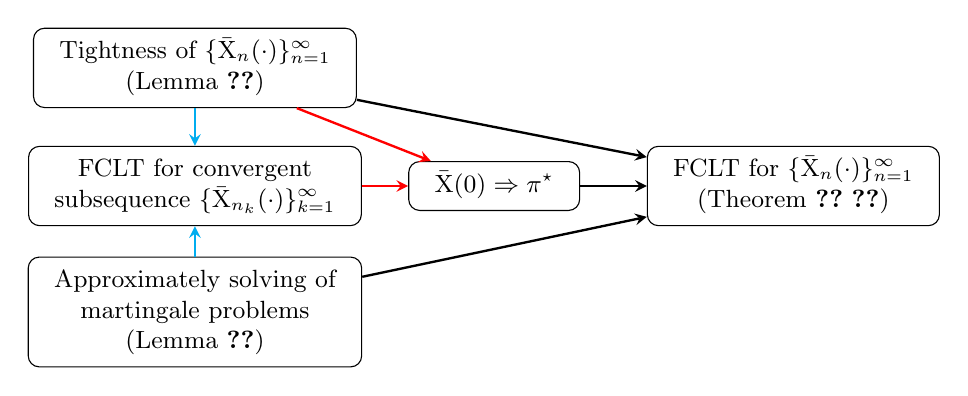
\begin{tikzpicture}[>=stealth,every node/.style={shape=rectangle,draw,rounded corners, minimum width=1cm, node distance=0.8cm},]
		
		\node (xtight) at (0,1.5) 		{\small \begin{tabular}{c}
				Tightness of $\{ \xbar_{n}(\cdot) \}_{n=1}^\infty$ \\
				(Lemma~\ref{lem:tight-twotime})
		\end{tabular}};
		\node (martprob) at (0,-1.6)
		{\small \begin{tabular}{c}
				Approximately solving of \\
				martingale problems \\
				(Lemma~\ref{lem:mart-prob-twotime})
		\end{tabular} };
		
		\node (subseq) at (0,0)
		{\small \begin{tabular}{c}
				FCLT for convergent \\ subsequence 
				$\{ \xbar_{n_k}(\cdot) \}_{k=1}^\infty$
		\end{tabular} };
	
		\draw[->, line width=.3mm, color=cyan] (xtight) to (subseq);
		\draw[->, line width=.3mm, color=cyan] (martprob) to (subseq);
	
	
		\node (xinitial) at (3.8,0)
		{\small \begin{tabular}{c}
				$\xbar(0) \weakconverge \pi^\star$
		\end{tabular}};
		
		\node (xfclt) at (7.6,0)
		{\small \begin{tabular}{c}
				FCLT for $\{ \xbar_{n}(\cdot) \}_{n=1}^\infty$ \\
				(Theorem~\ref{thm:fclt-twotime}~\ref{thm:fclt-x})
		\end{tabular} };
		
		\draw[->, line width=.3mm, color=red] (subseq) to  (xinitial);
		\draw[->, line width=.3mm, color=red] (xtight) to  (xinitial);
		\draw[->, line width=.3mm] (xinitial) to  (xfclt);
		\draw[->, line width=.3mm] (xtight) to (xfclt);
		\draw[->, line width=.3mm] (martprob) to (xfclt);
%		\draw[->, line width=.3mm] (ycheck) to (ytight);
		
	\end{tikzpicture}
	\caption{Illustration for the last step of proof.}
	\label{fig:proof-intergrate}
\end{figure}

We now briefly illustrate how Proposition~\ref{prop:mart-prob-approx} is applied with $\AM = \AM_x$ and $\uu_{n}(\cdot) = \xbar_{n}(\cdot)$ to derive the FCLT for $\xbar_{n}(\cdot)$ in Theorem~\ref{thm:fclt-twotime}. The process can be divided into three parts, corresponding to the cyan, red, and black arrows in \Figref{fig:proof-intergrate}.

\begin{enumerate}[(i)]
	\item \textbf{FCLT for convergent subsequences}:
	Conditions~\ref{prop:final:condition:unique}, \ref{prop:final:condition:tight}, and \ref{prop:final:condition:mart-prob} are verified in Section~\ref{sec:fclt:prelim}, Lemmas~\ref{lem:tight-twotime} and \ref{lem:mart-prob-twotime}, respectively. Tightness ensures the existence of a convergent subsequence, and applying Proposition~\ref{prop:mart-prob-approx} shows that the subsequence converges to a solution of \eqref{eq:fclt-twotime:x-sde}.
	
%Condition~\ref{prop:final:condition:unique} was discussed in Section~\ref{sec:fclt:prelim}.
%Condition~\ref{prop:final:condition:tight} is verified in Lemma~\eqref{lem:tight-twotime}.
%Condition~\ref{prop:final:condition:mart-prob} follows naturally from Lemma~\ref{lem:mart-prob-twotime}.
%By Proposition~\ref{prop:tight}, the tightness of $\xbar_{n}(\cdot)$ implies both the tightness of $\xbar_{n}(0)$ and the existence of a convergent subsequence ${\xbar_{n_k}(\cdot)}{k=1}^\infty$, along with the convergence of ${\xbar_{n_k}(0)}_{k=1}^\infty$. Suppose $\xbar_{n_k}(0) \weakconverge \tilde{\pi}$; applying Proposition~\ref{prop:mart-prob-approx} to this subsequence shows that $\xbar_{n_k}(\cdot)$ weakly converges to a solution of \eqref{eq:fclt-twotime:x-sde} with initial distribution $\tilde{\pi}$.
	
	\item \textbf{Convergence of initial distributions}: 
	Assumption~\ref{assump:hurwitz} guarantees both the uniqueness of the invariant distribution $\pi^\star$ and the geometric ergodicity for \eqref{eq:fclt-twotime:x-sde} (see Proposition~\ref{prop:ergo}). These properties ensure that all convergent subsequences of $\xbar_{n}(0)$ have the same limit $\pi^\star$, which implies the convergence of $\xbar_{n}(0)$.
	
%	Assumption~\ref{assump:hurwitz}, not previously invoked, plays a critical role here. It ensures both the uniqueness of the invariant distribution $\pi^\star$ for \eqref{eq:fclt-twotime:x-sde} and its geometric ergodicity (see Proposition~\ref{prop:ergo}). Using the FCLT for subsequences and geometric ergodicity, we establish the convergence of $\xbar_{n}(0)$. From the tightness of $\xbar_{n}(0)$, it suffices to verify that all convergent subsequences of $\xbar_{n}(0)$ converge to the same limit $\pi^\star$.
%	
%	Suppose $\xbar_{n_k}(0) \weakconverge \tilde{\pi}$. For a fixed $T > 0$, there exists $m_k$ such that $\xbar_{n_k}(0) = \xbar_{m_k}(T) + o_p(1)$. Without loss of generality, assume $\xbar_{m_k}$ weakly converges.
%	Letting $k \to \infty$, we have $\ermX(T) \sim \tilde{\pi} $, where $\ermX(t)$ is the solution to \eqref{eq:fclt-twotime:x-sde} with some initial distribution.
%	By the geometric ergodicity of \eqref{eq:fclt-twotime:x-sde}, for sufficiently large $T$, $\ermX(T) \approx \pi^\star$. Taking  $T \to \infty$ yields $\tilde{\pi} = \pi^\star$.
		
	\item \textbf{FCLT for the entire sequence}: Applying Proposition~\ref{prop:mart-prob-approx} to the full sequence establishes the desired FCLT.
\end{enumerate}
%The detailed proof is deferred to Appendix~\ref{sec:fclt:proof:intergrate}.
Similarly, we could obtain the following FCLT for $\zbar_{n}(\cdot)$.
\begin{cor}[FCLT for the auxiliary sequence]\label{cor:fclt-z}
	Under the conditions of Theorem~\ref{thm:fclt-twotime},
	the stochastic process $\zbar_{n}(\cdot)$ defined in \eqref{eq:zbar-short} converges weakly to the stationary solution of the SDE in \eqref{eq:fclt-twotime:y-sde}.
%	\begin{align}
%		%					\label{eq:fclt-twotime:y-sde}
%		d \ermY(t) = - \left(B_3 - \frac{\invdiffslow \mI}{2}  \right) \ermY(t) dt + \widetilde{\Sigma}_{\psi}^{1/2} d \ermW^{d_y}(t),
%	\end{align}
%	where $\widetilde{\Sigma}_{\psi}$ is defined in \eqref{eq:cov-z}.
\end{cor}

From the construction of $\ybar_{n}(\cdot)$ and $\zbar_{n}(\cdot)$ in \eqref{eq:ybar-short} and \eqref{eq:zbar-short}, it follows that their finite-dimensional distributions share the same weak convergence limits. Consequently, by Proposition~\ref{prop:tight}, $\ybar_{n}(\cdot)$ and $\zbar_{n}(\cdot)$ converge to the same limit. The detailed proof for this subsection and Corollary~\ref{cor:clt} is deferred to Appendix~\ref{sec:fclt:proof:intergrate}.


\section{Concluding Remarks}\label{sec:fclt:conclude}

In this paper, we have established decoupled FCLTs for two-time-scale SA, representing a significant advancement over prior single-point decoupled convergence results. Our results provide a more comprehensive characterization of the interdependence between different time scales. While the decoupling primarily pertains to the convergence rates, the limiting trajectory of the slow-time-scale update remains intrinsically influenced by the fast-time-scale update through the parameters in the associated limiting SDEs.

To achieve decoupled FCLTs, we have introduced a novel auxiliary sequence that effectively mitigates the primary influence of the fast-time-scale update on the slow-time-scale dynamics. We would believe this auxiliary sequence can serve as a useful tool for further investigations into two-time-scale algorithms.

Despite the progress presented in this work, several promising directions for future research remain open. First, extending our results to accommodate more general noise settings, such as Markovian or state-dependent noise, would be of significant interest. Second, establishing FCLTs for partial-sum processes of two-time-scale SA and leveraging these results for online inference presents another compelling avenue. Lastly, exploring scenarios involving more complex or heterogeneous time scales could further broaden the applicability of our framework.








% --- end tex/fclt.tex ---

\begin{appendix}
% --- begin tex/append.tex ---

\section{Additional Discussion on Assumptions}
%	Proofs for Section~\ref{sec:fclt:assump}}
\label{sec:fclt:proof:assump}

In this section, we discuss more details of the assumptions in Section~\ref{sec:fclt:assump} and present some useful properties  for our proof.

\subsection{Further Discussion}

Assumption~\ref{assump:smoothH} is equivalent to the H\"older continuity of $\nabla H$.

\begin{assumpt}{\ref*{assump:smoothH}$\dagger$}[$\Hsmooth$-H\"older continuity of $\nabla H$]
\label{assump:H:holder-assump}
Assume that $H(\cdot)$ is differentiable and there exist constants $\Hholder \ge 0$ and $\Hsmooth \in [0,1]$ such that $\forall \, y_1, y_2 \in \RB^{d_y}$, 
\begin{equation}
    \label{assump:H:holder}
    \| \nabla H(y_1) - \nabla H(y_2) \|
    \le \Hholder \| y_1 - y_2 \|^{\Hsmooth}.
\end{equation}
\end{assumpt}

\begin{prop}[{\cite[Proposition~B.1]{han2024finite}}]\label{prop:holder-equiv}
Suppose $\Hsmooth \in [0,1]$.
Under Assumption~\ref{assump:H:holder-assump},
Assumption~\ref{assump:smoothH} holds with $S_H = \frac{\Hholder}{1+\Hsmooth} $;
under Assumption~\ref{assump:smoothH}, Assumption~\ref{assump:H:holder-assump} holds with $\Hholder = 2^{1-\Hsmooth} \sqrt{1+\Hsmooth} \left( \frac{1+\Hsmooth}{\Hsmooth} \right)^\frac{\Hsmooth}{2} S_H$
%	\footnote{
    (we make the contention that $\left( \frac{1+\Hsmooth}{\Hsmooth} \right)^\frac{\Hsmooth}{2} = 1$ if $\Hsmooth = 0$). 
%		}
\end{prop}



%The proof of Proposition~\ref{prop:H-reduce-order} can be found in Section~\ref{sec:fclt:proof:assump}.

%An assumption closely related to Assumption~\ref{assump:smoothH} is the H\"older continuity of $\nabla H$.

%The two assumptions are equivalent, as shown in the following proposition.
% an upcoming proposition. This proposition extends Theorem 4.1 (Euclidean case) in \citet{berger2020quality} from scalar-valued functions to vector-valued functions. 
%Therefore, moving forward, we won't distinguish between these two assumptions.

The following propositions suggest that with the Lipschitz conditions, we can always select a lower order without compromising the validity of Assumptions~\ref{assump:smoothH} and \ref{assump:near-linear}.
Their proofs are deferred to Appendix~\ref{sec:fclt:proof:assump:proof}.

\begin{prop}\label{prop:H-reduce-order}
Suppose that \eqref{assump:smooth:FH:ineqH} holds.
If Assumption~\ref{assump:smoothH} holds up to order $1 + \Hsmooth$, then it also holds up to order $1+\Hsmooth'$ for any $\Hsmooth' \in [0, \Hsmooth] $.
\end{prop}

%Similar to Proposition~\ref{prop:H-reduce-order}, we have the following property.
\begin{prop}\label{prop:FG-reduce-order}
Suppose that Assumption~\ref{assump:smooth} holds.
If Assumption~\ref{assump:near-linear} holds up to order $(1+\Fsmooth, 1+\Gsmooth)$, then it also holds up to order $(1+\Fsmooth', 1+\Gsmooth')$ for any $\Fsmooth' \in (0, \Fsmooth)$ and $\Gsmooth' \in (0, \Gsmooth)$.
\end{prop}
%The proof of Proposition~\ref{prop:FG-reduce-order} can be found in Section~\ref{sec:fclt:proof:assump}.

%Propositions~\ref{prop:H-reduce-order} and \ref{prop:FG-reduce-order} suggest that with the Lipschitz conditions, we can always select a lower order without compromising the validity of Assumptions~\ref{assump:smoothH} and \ref{assump:near-linear}.
% As discussed in Section~\ref{sec:decouple:theo:step1}, 
%these local linearity assumptions entail the emergence of higher-order residual terms.
%The adjustments proposed in Propositions~\ref{prop:H-reduce-order} and \ref{prop:FG-reduce-order} enable us to choose an appropriate order, thereby preventing excessively high-order residual terms.

With Assumptions~\ref{assump:smoothH} and \ref{assump:near-linear}, we can decompose these operators as linear parts and higher-order residual terms.

\begin{prop}[Operator decomposition]
\label{prop:operator-decom}
Suppose that Assumptions~\ref{assump:smoothH} and \ref{assump:near-linear} hold.
With $\xhat_{n}$ and $\yhat_{n}$ defined in \eqref{alg:xyhat}, for any $\Fsmooth' \in (0, \Fsmooth]$, $\Gsmooth' \in (0, \Gsmooth]$ and $\Hsmooth' \in (0, \Hsmooth]$, we have the following results.
\begin{enumerate}[(i)]
    \item $F(\xx_{n}, \yy_{n}) = B_1 \xhat_{n} + R_{n}^F$ with $\|R_{n}^F\| = \OM( \| \xhat_{n} \|^{1+\Fsmooth'} + \| \yhat_{n} \|^{1+\Fsmooth'} )
    $.
    % $.
    \item $G(\xx_{n}, \yy_{n}) = B_2\xhat_{n} + B_3\yhat_{n} + R_{n}^{G}$ with $\|R_n^{G}\| = \OM( \| \xhat_{n} \|^{1+\Gsmooth'} + \| \yhat_{n} \|^{1+\Gsmooth'} )
    $. 
    \item $H(\yy_{n+1}) - H(\yy_{n}) = H^\star  (\yy_{n+1}-\yy_{n}) + R_{n}^{\nablaH} + R_{n}^H $ with $H^\star := \nabla H(\yy^\star)$, $\|R_{n}^H\| = \OM (\|\yy_{n+1}-\yy_{n}\|^{1+\Hsmooth'} )$ and $R_{n}^{\nablaH} =  (\nablaH(\yy_{n}) - \nablaH(\yy^{\star}))(\yy_{n+1}-\yy_{n})$.
\end{enumerate}
\end{prop}


\begin{rema}[Implications of Assumption~\ref{assump:stepsize-twotime}]\label{rema:step-size}
We can derive the following results from Assumption~\ref{assump:stepsize-twotime}.
\begin{itemize}
    \item
    Assumption~\ref{assump:stepsize-twotime} implies $\beta_n = \Omega(1/n)$ and $\alpha_{n} / \beta_{n} = \omega(1)$. Then we have
        $\ssum{n}{0}{\infty} \alpha_{n} = \ssum{n}{0}{\infty} \beta_{n} = \infty$,
    which is a ubiquitous condition in the SA analysis to ensure convergence to the target solution \citep{konda2004convergence, doan2022nonlinear, faizal2023functional}.
    
    \item 
     Note that $\alpha_{n+1}^{-1} - \alpha_{n}^{-1} = \beta_{n+1}^{-1} \kappa_{n+1} - \beta_{n}^{-1} \kappa_{n} = \beta_{n+1}^{-1} (\kappa_{n+1} - \kappa_{n}) + \kappa_{n} ( \beta_{n+1}^{-1} - \beta_{n}^{-1} ) = \beta_{n+1}^{-1} \kappa_{n+1} ( 1 - \kappa_{n} / \kappa_{n+1} ) + \kappa_{n} ( \beta_{n+1}^{-1} - \beta_{n}^{-1} ) $.
    % It follows that $ \invdifffast = \kappa_{\infty} \invdiffslow $. 
    If we define  $\invdifffast := \lim_{n \to \infty} (\alpha_{n+1}^{-1} - \alpha_{n}^{-1} )$ then we have $\invdifffast = 0$. 
    This is why the choice of step sizes does not affect the SDE in \eqref{eq:fclt-twotime:x-sde}.
    The parameters $\invdiffslow$ and $\invdifffast$ also frequently in previous analysis \citep{konda2004convergence, faizal2023functional}.
    % Then $\ssum{n}{0}{\infty} \beta_{n} = \infty$.
    % Since , it follows that $\ssum{n}{0}{\infty} \alpha_{n} = \infty$
\end{itemize}
\end{rema}

\begin{rema}[Linear case]
If $F$ and $G$ are linear operators, implying $H$ is also linear. the residual terms in Proposition~\ref{prop:operator-decom} vanish.
Under this scenario, for Lemmas~\ref{lem:check-twotime-xy} and \ref{lem:check-twotime-z}, as well as Theorem~\ref{thm:fclt-twotime}, to hold, Condition~\ref{assump:stepsize-twotime-moreab} in Assumption~\ref{assump:stepsize-twotime} is no longer necessary. Moreover, the requirement for the boundedness of fourth moments can be relaxed to $p$-th moments for any $p>2$.
For 
polynomially diminishing step sizes 
$\alpha_{n} = \alpha_{0} (n+1)^{-a}$ and $\beta_{n} = \beta_{0} (n+1)^{-b}$ with $a, b \in (0, 1]$, 
it suffices to ensure $b / a > 1$.
\end{rema}

\subsection{Proofs}
\label{sec:fclt:proof:assump:proof}

\begin{proof}[Proof of Proposition~\ref{prop:H-reduce-order}]
Combining \eqref{assump:smooth:FH:ineqH} and Assumption~\ref{assump:smoothH}, we have
\begin{equation*} 
    % \label{assump:H:smooth}
    \| H(y_1) -  H(y_2) - \nablaH(y_2) (y_1-y_2)  \| \le S_H \|y_1-y_2\| \cdot \min\left\{\|y_1-y_2\|^\Hsmooth, R_H \right\}
\end{equation*}
with $R_H = \frac{2L_H}{S_H}$.
For any $\Hsmooth' \in [0, \Hsmooth]$,
if $\| \yy_1 - \yy_2 \|^\Hsmooth \le R_H$, then we have 
\begin{equation*}
    \| H(\yy_1) - H(\yy_2) - \nablaH(\yy_2) (\yy_1-\yy_2) \| \le S_H R_H^{\Hsmooth - \Hsmooth'} \| \yy_1 - \yy_2 \|^{1+\Hsmooth'};
\end{equation*}
otherwise, we have
\begin{equation*}
    \| H(\yy_1) - H(\yy_2) - \nablaH(\yy_2) (\yy_1-\yy_2) \| \le S_H R_H \| \yy_1 - \yy_2 \| \le S_H R_H / R_H^{\Hsmooth'}  \| \yy_1 - \yy_2 \|^{1+\Hsmooth'}.
\end{equation*}
Thus, by replacing $S_H$ with $\max\left\{S_H R_H^{\Hsmooth - \Hsmooth'}, S_H R_H /  R_H^{\Hsmooth'} \right\}$,
Assumption~\ref{assump:smoothH} holds up to order $1+\Hsmooth'$.
\end{proof}

\begin{proof}[Proof of Proposition~\ref{prop:FG-reduce-order}]
For ease of exposition,  we let $\xhat = \xx - H(\yy)$ and $\yhat = \yy - \yy^\star$.
First, these assumptions imply
% $$ \|F(\xx, \yy) - B_1(\xx - H(\yy)) \| = \|F(\xx, \yy) - F(H(\yy), \yy) - B_1(\xx - H(\yy)) \| \le 2 L_F \| \xx - H(\yy) \|  $$ 
\begin{align*}
    \|F(\xx, \yy) - B_1 \xhat \| 
    & = \|F(\xx, \yy) - F(H(\yy), \yy) - B_1 \xhat  \| \le 2 L_F \| \xhat \| + \eps \cdot \| \yhat \|, \\
    \| G(\xx, \yy) - B_2 \xhat - B_3 \yhat ) \| 
    % \\
    & = \| G(\xx, \yy) - G(H(\yy), \yy) + G(H(\yy), \yy) - G(H(\yy^\star), \yy^\star) {-} B_2 \xhat {-} B_3 \yhat \| \\
    & \le 2 \LGx \| \xhat \| + 2 \LGy \| \yhat \|,
\end{align*} 
where $\eps$ is an arbitrary positive constant.
In the following, we only prove that \eqref{assump:near-linear-G} holds after  replacing $\Gsmooth$ with $\Gsmooth' \in (0, \Gsmooth)$.
The proof for \eqref{assump:near-linear-F} is similar.

If (i) $ \SBG \| \xhat \|^{1+\Gsmooth} \le 2 \LGx \| \xhat \| $ and $\SBG \| 
\yhat \|^{1+\Gsmooth} \le 2 \LGy \| \yhat \| $ 
or (ii) $ \SBG \| \xhat \|^{1+\Gsmooth} > 2 \LGx \| \xhat \| $ and $\SBG \| 
\yhat \|^{1+\Gsmooth} > 2 \LGy \| \yhat \| $,
we have
\begin{align*}
    \| G(\xx, \yy) - B_2 \xhat - B_3 \yhat ) \|
    & \le \min \left\{ \SBG \| \xhat \|^{1+\Gsmooth} + \SBG \| \yhat \|^{1+\Gsmooth}, 2 \LGx \| \xhat \| + 2 \LGy \| \yhat \| \right\} \\
    & = \min \left\{ \SBG \| \xhat \|^{1+\Gsmooth}, 2 \LGx \| \xhat \| \right\} + \min \left\{ \SBG \| \yhat \|^{1+\Gsmooth}, 2 \LGy \| \yhat \|  \right\} \\
    & = \SBG \| \xhat \| \cdot \min\left\{ \| \xhat \|^\Gsmooth, \frac{2 \LGx}{\SBG} \right\} + \SBG \| \yhat \| \cdot \min \left\{ \| \yhat \|^{\Gsmooth}, \frac{2\LGy}{\SBG} \right\}.
\end{align*}
Then the remaining proof is similar to that of Proposition~\ref{prop:H-reduce-order}.

If neither of (i) and (ii) holds, without loss of generality we assume $ \SBG \| \xhat \|^{1+\Gsmooth} \le 2 \LGx \| \xhat \| $ and $\SBG \| 
\yhat \|^{1+\Gsmooth} > 2 \LGy \| \yhat \| $.
This implies $ \| \xhat \| \le c_x := (2 \LGx / \SBG)^{1/\Gsmooth}  $ and $\| \yhat \| > c_y := ( 2 \LGy / \SBG )^{1/\Gsmooth}$.
Then we have 
\begin{align*}
    \| G(\xx, \yy) - B_2 \xhat - B_3 \yhat ) \|
    & \le \min \left\{ \SBG \| \xhat \|^{1+\Gsmooth} + \SBG \| \yhat \|^{1+\Gsmooth}, 2 \LGx \| \xhat \| + 2 \LGy \| \yhat \| \right\} \\
    & \le 2 \LGx \| \xhat \| + 2 \LGy \| \yhat \| 
    % & \le \min \left\{ \SBG \, c_x^{1+\Gsmooth} + \SBG \| \yhat \|^{1+\Gsmooth}, 2 \LGx\, c_x + 2 \LGy \| \yhat \| \right\} \\
    \le  2 \LGx\, c_x + 2 \LGy \| \yhat \| \\
    & \le \left( \frac{2 \LGx c_x}{ c_y^{1+\Gsmooth'} } + \frac{2 \LGy}{c_y^{\Gsmooth'}} \right) \| \yhat \|^{1+\Gsmooth'}.
\end{align*}
Thus \eqref{assump:near-linear-G} holds with $\Gsmooth$ and $\SBG$ replaced with $\Gsmooth'$ and $\frac{2 \LGx c_x}{ c_y^{1+\Gsmooth'} } + \frac{2 \LGy}{c_y^{\Gsmooth'}}$ respectively.
\end{proof}



\section{Omitted Details for Section~\ref{sec:fclt:main}}\label{append:construct}
In this section, we present more details for the construction in Section~\ref{sec:fclt:construct} and the examples in Section~\ref{sec:fclt:exam}.

\subsection{Non-asymptotic Convergence Rates}\label{append:construct-non-asymp}
We first give the formal statement of Proposition~\ref{prop:mart-decouple-rate}.

\begin{prop}[Non-asymptotic convergence rates, {\cite[Theorem~3.1]{han2024finite}}]\label{prop:mart-decouple-rate-formal}
Suppose that Assumptions~\ref{assump:smooth} -- \ref{assump:noise-fclt} and the following strong monotonicity conditions hold:
(i) there exists a constant $\mu_{F} > 0$ such that for any $y \in \RB^{d_y}$ and $x \in \RB^{d_x}$, 
%	\begin{align}
    $\left\langle x - H(y), F(x,y) - F(H(y),y) \right\rangle \geq \mu_{F} \|x-H(y)\|^2$;
    %		 \quad \forall\, x \in \RB^{d_x}. 
    %		\label{assump:sm:F:ineq}    
    %	\end{align}
%	$G(H(\cdot), \cdot)$ is strongly monotone at $y^{\star}$, i.e., 
(ii) there exists a constant $\mu_{G} > 0$ such that for any $ y\in\RB^{d_y}$,
%	\begin{align}
    $\left\langle y - y^{\star}, G(H(y),y) - G(H(y^\star), y^\star) \right\rangle \geq \mu_{G} \|y - y^{\star}\|^2$.
    %		\quad \forall\, y\in\RB^{d_y}. \label{assump:G:sm}    
    %	\end{align}
Then we have $\EB \| \xhat_{n} \|^4 + \EB \| \yhat_{n} \|^4 = \OM (\alpha_{n}^2)$.
If we further assume $b/a \le 1 + \Fsmooth/2$ in the step size selection of Example~\ref{exmp:fclt-stepsize}, we have $\EB \| \xhat_{n} \|^2 = \OM(\alpha_{n}) $ and $\EB \| \yhat_{n} \|^2 = \OM(\beta_{n})$.
\end{prop}
Regarding the comparison between strong monotonicity and Assumption~\ref{assump:hurwitz}, strong monotonicity is a non-asymptotic condition that guarantees convergence from arbitrary initializations, whereas Assumption~\ref{assump:hurwitz} is a local condition that guarantees only the asymptotic behavior.
As for the additional requirement for the step sizes, we guess that this is due to proof techniques in \cite{han2024finite} and is not inherent to the problem itself.


\subsection{Details for the Construction}\label{append:construct-details}
In this subsection, we present an equivalent expression of the construction in \eqref{eq:xbar-short}, \eqref{eq:ybar-short} and \eqref{eq:zbar-short} for ease of subsequent proof.
We first introduce some necessary notation inspired by \cite{gadat2018stochastic, liang2023asymptotic}.
\begin{defn}[Time interpolation]\label{defn:time-inter}
For the step size sequences $\{ \alpha_{n} \}_{n=0}^\infty$ and $\{ \beta_{n} \}_{n=0}^\infty$, $n, n' \in \NB$ with $n' > n$ and $t \ge 0$, we define
% (we let $\ssum{k}{n}{n-1} \alpha_{k} = 0 $), define
% (change the order of the first two definitions)
\begin{align*}
    \Gamma^\alpha_{n, n'} := \ssum{k}{n}{n'-1} \alpha_{k},\ 
    N^\alpha(n, t) := \max \left\{ m \ge n \colon \Gamma^\alpha_{n, m} \le t \right\}, 
    \ \text{ and } \
    \underline{t}^\alpha_{n} = \Gamma^\alpha_{n, N^\alpha(n,t)} 
    % = \max\{ t' = \Gamma^\alpha_{n, m} \text{ for some } m \colon: t' \le t \}
    , \\
    % \text{ or } N^\alpha(n, t) := \max \left\{ m \ge n \colon \Gamma^\alpha_{n, m} \le t \right\} \\
    \Gamma^\beta_{n, n'} := \ssum{k}{n}{n'-1} \beta_{k}, \ N^\beta(n, t) := \max \left\{ m \ge n \colon \Gamma^\beta_{n,m} \le t \right\}, \ 
    \text{ and } \
    \underline{t}^\beta_{n} = \Gamma^\beta_{n, N^\beta(n,t)}.
    % N^\alpha(n, t) := \min \left\{ m \ge n \colon \ssum{k}{n}{m} \alpha_{k} > t \right\}, \ 
    % \Gamma^\alpha_{n, n'} := \ssum{k}{n}{n'-1} \alpha_{k}, \ \text{ and } \
    % \underline{t}^\alpha_{n} = \Gamma^\alpha_{n, N^\alpha(n,t)}, \\
    % N^\beta(n, t) := \min \left\{ m \ge n \colon \ssum{k}{n}{m} \beta_{k} > t \right\}, \ 
    % \Gamma^\beta_{n, n'} := \ssum{k}{n}{n'-1} \beta_{k}, \ \text{ and } \
    % \underline{t}^\beta_{n} = \Gamma^\beta_{n, N^\beta(n,t)}.
\end{align*}
For $n' \le n$, we stipulate $\Gamma^\alpha_{n,n'} = \Gamma^\beta_{n,n'}  := 0 $.
\end{defn}

\begin{fact}
Under Definition~\ref{defn:time-inter}, we have the following properties. 
\begin{enumerate}[(i)]
    \item For $n_1 \le n_2 \le n_3$, $\Gamma^\alpha_{n_1, n_2} + \Gamma^\alpha_{n_2, n_3} = \Gamma^\alpha_{n_1, n_3}$. 
    \item 
%		$N^\alpha(n, t) = \max \left\{ m \ge n \colon \Gamma^\alpha_{n, m} \le t \right\}$ and 
    For $m \ge n$, $N^\alpha(n, \Gamma^\alpha_{n,m}) = m $.
    \item $\underline{t}^\alpha_{n} \le t <  \underline{t}^\alpha_{n} + \alpha_{N^\alpha(n,t)} $. When $t = \Gamma^\alpha_{n, m}$ for some $m \ge n$, $t = \underline{t}^\alpha_{n} $.
    \item  As $n \to \infty$, if $\alpha_{n} \to 0 $, then $\underline{t}^\alpha_{n} \uparrow t$.
\end{enumerate}
Similar properties hold if the superscript is replaced by $\beta$.
\end{fact}

In other words,
$\Gamma^\alpha_{n, n'}$ denotes the accumulation of the step sizes from $n$-th iteration to $(n'-1)$-th iteration.
% $N^\alpha(n, t)$ denotes the minimal iteration such that the accumulation of step sizes from $n$-th iteration is larger than $t$.
% In other words, 
$N^\alpha(n, t)$ is the maximal integer such that $\Gamma^\alpha_{n, N^\alpha(n, t)} \le t $.
We define this value by $\underline{t}^\alpha_{n} $,
which can be viewed as an approximation of $t$ from the left.
% Then we define $\underline{t}^\alpha_{n} $ 
% as an approximation (below) of $t$ when we only consider the discontinuous points from the step sizes(?) (or, when we consider the discretization).
% Since $\alpha_{n} \to 0$, we have $\underline{t}^\alpha_{n} \uparrow t$ as $n \to \infty$.
% ($\underline{t}^\alpha_{n} \le t \le  \underline{t}^\alpha_{n} + \alpha_{N^\alpha(n,t)} $)


% We introduce some additional definitions.
% Define the accumulation of step sizes as follows.
% \begin{align}
%     \Gamma^\alpha_{n, n'} := \ssum{k}{n}{n'-1} \alpha_{k},\ 
%     \Gamma^\beta_{n, n'} := \ssum{k}{n}{n'-1} \beta_{k},
% \end{align}

The following lemma characterizes the magnitude of $N^\alpha(n,t)$ and $N^\beta(n,t)$. 
\begin{lem}\label{lem:aux:bounded}
Suppose that Assumption~\ref{assump:stepsize-twotime} holds.
There exist two positive constants $c_\alpha$ and $c_\beta$ such that for any $t>0$ and $n \in \NB$,
\begin{equation*}
    n \le N^\alpha(n,t) \le 2^{ \left\lceil 2t/c_\alpha \right\rceil + 1} n \quad \text{ and } \quad 
    n \le N^\beta(n,t) \le 2^{ \left\lceil 2t/c_\beta \right\rceil + 1} n.
\end{equation*}
As a corollary, 
$\frac{\alpha_{n}}{ \alpha_{N^\alpha (n, t) } } 
% \le \frac{ N^\alpha(n,t) }{n} 
\le 2^{ \left\lceil 2t/c_\alpha \right\rceil + 1}$ and $\frac{\beta_{n}}{ \beta_{N^\beta (n, t) } } 
% \le \frac{ N^\beta(n,t) }{n} 
\le 2^{ \left\lceil 2t/c_\beta \right\rceil + 1}$.
\end{lem}

Lemma~\ref{lem:aux:bounded} shows that under our assumptions, both $N^\alpha(n,t)$ and $N^\beta(n,t)$ are of the order $\Theta(n)$. This property is useful for establishing the tightness in Section~\ref{sec:fclt:tight}. The proof of Lemma~\ref{lem:aux:bounded} is deferred to the end of this subsection. 

With Definition~\ref{defn:time-inter}, the construction in \eqref{eq:xbar-short}, \eqref{eq:ybar-short} and \eqref{eq:zbar-short} can be equivalently expressed as follows

%Now we construct continuous random functions $\xbar_{n}(\cdot)$, $\ybar_{n}(\cdot)$ and $\zbar_{n}(\cdot)$.
%We first focus on $\xbar_{n}(\cdot)$.
%The function $\xbar_{n}(\cdot)$ starts from $\xbar_{n}(0) = \xcheck_{n}$ and passes through $\xcheck_{n+1}$, $\xcheck_{n+2}$ and so on as $t$ increases.
%We place $\{ \xcheck_{n+k} \}_{k=0}^\infty$ on the time sequence $\{ \Gamma^\alpha_{n, n+1-k} \}_{k=0}^\infty$,
%% This process starts from $\xcheck_{n}$.
%i.e., 
%% for $t \in \{ \Gamma^\alpha_{n, n+k} \}_{k \ge 1}$, 
\begin{align}\label{eq:def:xbar}
\begin{split}
    \xbar_{n}(t) 
    & \overset{\eqref{eq:xbar-short}}{=} \xcheck_{ N^\alpha(n,t) } + \frac{t - \underline{t}^\alpha_{n}}{ \alpha_{N^\alpha(n,t)} } \big( \xcheck_{ N^\alpha(n,t) + 1} - \xcheck_{ N^\alpha(n,t)  } \big) \\
    & \overset{\eqref{eq:xcheck-twotime}}{=} \xcheck_{ N^\alpha(n,t) } + (t - \underline{t}^\alpha_{n} ) \left( - B_1 \xcheck_{N^\alpha(n,t)} + \frac{R_{N^\alpha(n,t)}^x}{ \alpha_{N^\alpha(n,t)} } \right) - \frac{t - \underline{t}^\alpha_{n}}{ \sqrt{ \alpha_{N^\alpha(n,t)} } } 
    %    \sqrt{ t - \underline{t}^\alpha_{n} }\,
    \tilde{\xi}_{N^\alpha(n,t)}.
\end{split} \\
\label{eq:def:ybar}
\begin{split}
    \ybar_{n}(t) 
    & \overset{\eqref{eq:ybar-short}}{=} \ycheck_{ N^\beta(n,t) } + \frac{t - \underline{t}^\beta_{n}}{\beta_{N^\beta(n,t)}} \big( \ycheck_{ N^\beta(n,t)+1 } - \ycheck_{ N^\beta(n,t) } \big) \\
    & \overset{\eqref{eq:ycheck-twotime}}{=} \ycheck_{ N^\beta(n,t) } + (t - \underline{t}^\beta_{n} ) \left[ \Big(- B_3 + \frac{\invdiffslow \mI}{2} 
    \Big) \ycheck_{N^\beta(n,t)} + \frac{R_{N^\beta(n,t)}^y }{ \beta_{N^\beta(n,t)} } \right] - 
    \frac{t - \underline{t}^\beta_{n}} {\sqrt{ \beta_{N^\beta(n,t)} } }
    \psi_{N^\beta(n,t)} 
    \\
    & \qquad - (t - \underline{t}^\beta_{n}) \sqrt{ \frac{ \alpha_{N^\beta(n,t)} }{ \beta_{N^\beta(n,t)} } } B_2 \xcheck_{N^\beta(n,t)}.
\end{split}\\
\label{eq:def:zbar}
\begin{split}
    \zbar_{n}(t) 
    & \overset{\eqref{eq:zbar-short}}{=} \zcheck_{ N^\beta(n,t) } + \frac{t - \underline{t}^\beta_{n}}{\beta_{N^\beta(n,t)}} \big( \zcheck_{ N^\beta(n,t)+1 } - \zcheck_{ N^\beta(n,t) } \big) \\
    & \overset{\eqref{eq:zcheck-twotime}}{=} \zcheck_{ N^\beta(n,t) } + (t - \underline{t}^\beta_{n} ) \left[ \Big(- B_3 + \frac{\invdiffslow \mI}{2} 
    \Big) \zcheck_{N^\beta(n,t)} + \frac{R_{N^\beta(n,t)}^z }{ \beta_{N^\beta(n,t)} } \right] -  \frac{t - \underline{t}^\beta_{n}}{ \sqrt{ \beta_{N^\beta(n,t)}} } 
    %    \sqrt{ t - \underline{t}^\beta_{n} }\, 
    \tilde{\psi}_{N^\beta(n,t)}.
\end{split}
\end{align}
%In particular, we have
% $\xbar_{n}(t) = \xbar_{n}(\Gamma^\alpha_{n, n+k} ) = \xcheck_{n+k-1} $, $\xbar_{n}(t) = \xbar_{n}(\Gamma^\alpha_{n, n+k} ) = \xcheck_{n+k} $

\begin{fact}\label{fact2}
Under Definition~\ref{defn:time-inter},
    $\xbar_{n}(\cdot)$	
% the construction in \eqref{eq:xbar-short} 
satisfies the following properties.
\begin{enumerate}[(i)]
    \item For $m \ge n$, $ \xbar_{n}(\Gamma^\alpha_{n, m} ) = \xcheck_{m}$.
    \item 	$\xbar_{n}(t) = \xbar_{n}( \underline{t}_n^\alpha ) + \frac{t - \underline{t}^\alpha_{n}}{ \alpha_{N^\alpha(n,t)} } \big(  \xbar_{n}( \underline{t}_n^\alpha + \alpha_{N^\alpha(n,t)} ) - \xbar_{n}( \underline{t}_n^\alpha ) \big)$.
    \item \label{fact2-3} For $m \ge n$ and $t \in [\Gamma^\alpha_{n,m}, \Gamma^\alpha_{n,m+1})$, $\xbar_{n}(\underline{t}^\alpha_{n}) = \xcheck_{m}$.
\end{enumerate}
Similar results also hold for $\ybar_{n}(\cdot)$ and $\zbar_{n}(\cdot)$.
\end{fact}
%For the general $t \ge 0$, we 
%we consider the following linear interpolation

\begin{rema}[Discussion on the interpolation]
For the way of interpolation in our works, \cite{faizal2023functional} also adopts the linear interpolation while \cite{gadat2018stochastic, liang2023asymptotic, blanchet2024limit} uses two different interpolations for different parts.
Since both $\alpha_{N^\alpha(n,t)}$ and $\beta_{N^\beta(n,t)}$ converge to $0$ as $n \to \infty$, different interpolation methods make no difference in the asymptotic sense in our setup. We choose simple linear interpolation for analytical simplicity such that each trajectory is continuous in time.
\end{rema}




\begin{proof}[Proof of Lemma~\ref{lem:aux:bounded}]
We first prove the result for the sequence $\{ \beta_{n} \}$.
From the definition of $N^\beta(n,t)$ in Definition~\ref{defn:time-inter}, we must have $N^\beta(n,t) \ge n$.
Then the monotonicity of $n \beta_{n}$ in Assumption~\ref{assump:stepsize-twotime} implies $\frac{\beta_{n}}{ \beta_{ N^\beta(n,t) } } \le \frac{ N^\beta(n,t) }{n}$. It remains to derive the upper bound of $\frac{ N^\beta(n,t) }{n} $.

% Next, we derive the upper bound on $\frac{ N^\beta(n,t) }{n} $.
From Assumption~\ref{assump:stepsize-twotime}, we have 
$\frac{ \beta_{n-1} }{ \beta_{n} } = 1 + \OM (\beta_{n}) = 1 + \OM (\beta_{n-1}) $.
It follows that $\frac{1}{\beta_{n}} = \frac{1}{\beta_{n-1}} + \OM(1) = \dots = \OM(n) $, implying $\beta_{n} = \Omega \big( \frac{1}{n} \big)$.
Consequently, 
there exists $c_\beta$ such that $\beta_{n} \ge \frac{c_\beta}{n} $ for any $n \in \NB$.
Meanwhile, for a fixed $n$, there exists a unique integer $k(n)$ such that $ 2^{k(n) - 1} \le n < 2^{k(n)} $.
Then we have that for any $k' \ge k(n)$,
% $\beta_{2^{k(n)} + 1} + \dots + \beta_{ 2^{k(n) + 1} } \ge  $
\begin{equation*}
    \beta_{2^{k'} + 1} + \dots + \beta_{ 2^{k' + 1} }
    \ge c_\beta \left( \frac{1}{ 2^{k'} + 1 } + \frac{1}{ 2^{k'} + 2 } + \dots \frac{1}{ 2^{k'+1} } \right)
    \ge \frac{ c_\beta }{2}.
\end{equation*}
It follows that with $m(n) := 2^{ k(n) + \left\lceil 2t/ c_\beta \right\rceil } $,
\begin{equation*}
    \Gamma^\beta_{n, m(n)+1}
    = \ssum{l}{n}{m(n)} \beta_{l}
    > \ssum{l}{2^{k(n)}+1}{2^{k(n) + \left\lceil 2t/c_\beta \right\rceil } } \beta_{l}
    \ge \left\lceil \frac{2t}{c_\beta} \right\rceil \frac{c_\beta}{2} \ge t.
\end{equation*}
From Definition~\ref{defn:time-inter}, we have $N^\beta(n,t) \le m(n) = 2^{ k(n) + \left\lceil 2t/c_\beta \right\rceil }$.
Recall that $n \ge 2^{k(n)-1}$. It follows that $\frac{ N^\beta(n,t) }{n} \le 2^{ \left\lceil 2t/c_\beta \right\rceil + 1 }$.

For the sequence $\{ \alpha_{n} \}$, Assumption~\ref{assump:stepsize-twotime} guarantees that $n \alpha_{n}$ is non-decreasing and $\frac{\alpha_{n-1}}{\alpha_{n}} = 1 + o(\beta_{n}) = 1 + \OM(\alpha_{n})$.
Then following similar procedure, we have that there exists $c_\alpha > 0$ such that $ \frac{ \alpha_{n} }{ \alpha_{ N^\alpha(n,t) } } \le \frac{ N^\alpha(n,t) }{n} \le 2^{ \left\lceil 2t/c_\alpha \right\rceil + 1 }$.
\end{proof}

\subsection{Details for Example~\ref{exmp:gtd}}
\label{append:exmp}

Consider an infinite-horizon MDP $\MM=(\SM, \AM, \PM ,r, \gamma)$ with discounted rewards, where $\SM$ and $\AM$ denote the (finite) state space and action space, respectively, and $\gamma \in [0,1)$ is the discount factor.
The transition kernel $\PM \colon \SM \times \AM \rightarrow \Delta(\SM)$ specifies the probability distribution over the next states for each state-action pair $(s,a) \in \SM \times \AM$, where $\PM(\cdot | s,a) \in \Delta(\SM) $ denotes the distribution of transitions from state $s$ when action $a$ is executed. The reward function $r\colon \SM \times \AM \rightarrow [0,1]$ represents the immediate reward received from state $s$ when action $a$ is taken.

A policy $\pi\colon \SM \rightarrow \Delta(\AM)$ maps each state to a probability distribution over actions. Its quality is assessed via the value function  $$V^\pi(s) := \EB \bigg[ \sum_{t=0}^\infty \gamma^t r(s_t, a_t) \,|\, s_0 = s,\ a_t \sim \pi(\cdot|a_t),\ s_{t+1} \sim \PM(\cdot|s_t,a_t) \bigg], $$
which gives the expected discounted cumulative reward for following policy $\pi$. 
The process of estimating $V^\pi$ for a fixed policy $\pi$ is known as \textit{policy evaluation}.
When the data is generated under a different policy $\pi_b$ to establish the value function $V^\pi$ of $\pi$, the task is referred to as \textit{off-policy evaluation}~\citep{uehara2022review}.
When $|\SM|$ is large, directly estimating $V^\pi$ becomes computationally infeasible. Instead, $V^\pi$ can be approximated using a parameterized function. A straightforward approach is linear function approximation, where
$V^\pi(s) \approx V(s;y) = \phi(s)^\top y$, with $\phi(s)$ representing the feature vector of state $s$~\citep{dann2014policy}.

To find the optimal parameter $y$, both GTD2 are TDC are derived by minimizing the
\textit{mean squared projected Bellman error} through SGD~\cite{sutton2009fast}.
In Example~\ref{exmp:gtd},
given the following i.i.d. samples $\{ (s_n, a_n, r(s_n, a_n), s'_{n}) \}_{n=0}^\infty$ with $a_n \sim \pi_b(\cdot | s_n)$ and $s'_{n} \sim \PM(\cdot|s_{n}, a_{n})$, we define $r_{n} = r(s_n, a_n)$, and $\rho_{n} = \frac{\pi(a_n|s_n)}{\pi_b(a_n|s_n)}$.
Note in this setting $s'_n$ does not necessarily equal $s_{n+1}$.
The importance weight $\rho_{n}$ adjusts for the mismatch between $\pi$ and $\pi_b$.
This weight does not appear in the original formulations of GTD2 and TDC in~\cite{sutton2009fast} due to the use of a sub-sampling procedure~\citep{maei2011gradient}.
We incorporate this weight in update rules \eqref{eq:gtd-x}--\eqref{eq:tdc-y} to align with subsequent works, e.g.,~\cite{xu2019two, li2024high}.

As discussed in Remark~\ref{rema:fclt}, deriving $\widetilde{\Sigma}_{\psi}$ in \eqref{eq:fclt-twotime:y-sde} requires analyzing the asymptotic covariance of $\psi_{n} - B_2 B_1^{-1} \xi_{n} $.
Suppose $(x_n, y_n)$ converges to $(x^\star, y^\star)$ in probability, as guaranteed by the results in~\cite{maei2011gradient}. For GTD2, we have $B_1 = C$ and $B_2 = -A^\top$, leading to
\begin{align*}
\psia_{n} - B_2 B_1^{-1} \xi_{n} 
& = -(A_{n}^\top {-} A^\top) x_{n} + A^\top C^{-1} [ (C_n {-} C) x_{n} + (A_n {-} A)y_{n} - (b_{n} {-} b) ] \\
& = A^\top C^{-1} ( A_{n} A^{-1} b - b_{n} ) + o_p(1)
\end{align*}

%	$\psia_{n} - B_2 B_1^{-1} \xi_{n} = -(A_{n}^\top - A^\top) x_{n} + A^\top C^{-1} [ (C_n - C) x_{n} + (A_n - A)y_{n} - b_{n} + b ] = A^\top C^{-1} ( A_{n} A^{-1} b - b_{n} ) + o_p(1)$.
For TDC, $B_1 = C$ and $B_2 = D^\top = C-A^\top$.
Then
%	Then $\psib_{n} = (D_n^\top - D^\top) x_{n} + (A_{n} - A ) y_{n} - b_{n}+b +A^\top C^{-1} [ (C_n - C) x_{n} + (A_n - A)y_{n} - b_{n} + b ] $
\begin{align*}
\psib_{n} - B_2 B_1^{-1}\xi_{n} 
& = (D_n^\top {-} D^\top) x_{n} + (A_{n} {-} A ) y_{n} - (b_{n} {-} b) \\
& \quad  \ - (C - A^\top) C^{-1} [ (C_n {-} C) x_{n} + (A_n {-} A)y_{n} - (b_{n} {-} b) ] \\
& = A^\top C^{-1} ( A_{n} A^{-1} b - b_{n} ) + o_p(1).
\end{align*}
Thus, both GTD2 and TDC share the same $\widetilde{\Sigma}_{\psi}$.




\section{Omitted Proofs}

\subsection{Proofs in Section~\ref{sec:fclt:one-step}}
\label{sec:fclt:proof:construct}
In this subsection, we give the proof of the one-step recursions in Section~\ref{sec:fclt:one-step}.
Since the proofs of both Lemmas~\ref{lem:check-twotime-xy} and \ref{lem:check-twotime-z} are closely related, we combine their proof together.
\begin{proof}[Proof of Lemmas~\ref{lem:check-twotime-xy} and \ref{lem:check-twotime-z}]
The proof is structured into three parts:  we derive the one-step recursion first for $\ycheck_{n}$, followed by $\xcheck_{n}$, and finally $\zcheck_{n}$.
To begin, we take the update rules for $\xhat_{n}$ and $\yhat_{n}$, as outlined below.
\begin{align}
    \xhat_{n+1} & = \xhat_n - \alpha_n F(x_n, y_n) - \alpha_n \xi_n + H(y_n) - H(y_{n+1}), \label{eq:xhat} \\
    \yhat_{n+1} & = \yhat_n - \beta_n G(H(y_n), y_n) + \beta_n ( G(H(y_n), y_n) - G(x_n, y_n) ) - \beta_n \psi_n. \label{eq:yhat}
\end{align}

\textbf{Part 1: one-step recursion for $\ycheck_{n}$}.
% We first derive the update rule of $\ycheck_{n}$. 
By Proposition~\ref{prop:operator-decom}, we can rewrite the update rule of $\yhat_{n}$ in \eqref{eq:yhat} as 
\begin{align}
    \label{eq:yhat-decom}
    \yhat_{n+1} = (I - \beta_{n} B_3) \yhat_{n} - \beta_{n} B_2 \xhat_{n} - \beta_n \psi_n - \beta_n R_n^G.
\end{align}
Then from the definition of $\ycheck_{n}$ and \eqref{eq:yhat-decom}, we have 
\begin{align}
    \ycheck_{n+1}
    & = \sqrt{ \frac{ \beta_{n-1} }{ \beta_{n} } } (\mI - \beta_{n} B_3) \ycheck_{n} - \sqrt{ \beta_{n} \alpha_{n-1} } B_2 \xcheck_{n} - \sqrt{\beta_{n}} \psi_{n} - \sqrt{\beta_{n}} R_{n}^G \nonumber \\
    & = \left( \mI - \beta_{n} B_3 + \frac{ \invdiffslow \beta_{n} }{2} \mI \right) \ycheck_{n} - \sqrt{\beta_{n} \alpha_{n} } B_2 \xcheck_{n} - \sqrt{\beta_n} \psi_{n} + R_{n}^y, \label{eq:lem:check-twotime:y-update}
\end{align}
where
\begin{align}\label{eq:lem:check-twotime:Ry}
    \begin{split}
        R_{n}^y
        & =  \underbrace{ \left( \sqrt{ \frac{ \beta_{n-1} }{\beta_{n}} } - 1 - \frac{ \invdiffslow \beta_{n} }{2} \right) \ycheck_{n} }_{=: R_{n,1}^y}  
        + \underbrace{ ( \beta_{n} - \sqrt{ \beta_{n} \beta_{n-1} } ) B_3 \ycheck_{n} 
            \vphantom{ \left( \sqrt{ \frac{ \beta_{n-1} }{\beta_{n}} } \right) } }_{ =:R_{n,2}^y } \\
        & \quad \  + \underbrace{
            % \sqrt{\beta_{n}} 
            ( \sqrt{ 
                \beta_{n} 
                \alpha_{n} } - \sqrt{ 
                \beta_{n} 
                \alpha_{n-1} } ) B_2 \xcheck_{n}
            \vphantom{ \left( \sqrt{ \frac{ \beta_{n-1} }{\beta_{n}} } \right) } }_{=: R_{n,3}^y } 
        - \underbrace{ \sqrt{\beta_{n}} R_{n}^G 
            \vphantom{ \left( \sqrt{ \frac{ \beta_{n-1} }{\beta_{n}} } \right) } }_{ =: R_{n,4}^y }.
    \end{split}
\end{align}
By Assumption~\ref{assump:stepsize-twotime}, we have
\begin{align}
    %		\begin{aligned} 
        \sqrt{ \frac{ \beta_{n-1} }{ \beta_{n} } } 
        & = \sqrt{ 1 + \beta_{n-1} ( \beta_{n}^{-1} - \beta_{n-1}^{-1} ) } = \sqrt{1 + \invdiffslow \beta_{n-1}  + o(\beta_{n-1}) } \nonumber \\
        & = \sqrt{1 + \invdiffslow \beta_{n}  + o(\beta_{n}) }
        = 1 + \frac{ \invdiffslow \beta_{n} }{2} + o(\beta_{n}), \nonumber \\
        \sqrt{ \frac{ \alpha_{n-1} }{\alpha_{n}} } 
        & = 1 + \OM(\beta_n),
        \qquad 
        \sqrt{ \frac{ \kappa_{n-1} }{\kappa_{n}} } 
        = 1 + \OM(\beta_n). \label{eq:lem:check-twotime:sqrtalpha}
        %		\end{aligned}
\end{align}
It follows that $\| R_{n,1}^y \| +  \| R_{n,2}^y \| = o(\beta_{n}) \| \ycheck_{n} \| = o(\beta_{n}^{1/2}) \| \yhat_{n} \|  $
and  $\| R_{n,3}^y \| = \OM(\beta_{n}^{3/2} \alpha_{n}^{1/2}) \| \xcheck_{n} \| = o(\beta_{n}^{3/2}) \| \xhat_{n} \| $. 
Meanwhile, by Proposition~\ref{prop:operator-decom}, we have $ \| R_{n,4}^y \| = \OM(\beta_{n}^{1/2}) ( \| \xhat_{n} \|^{1+\Gsmooth} + \| \yhat_{n} \|^{1+\Gsmooth} ) $.
Note that in Assumption~\ref{assump:stepsize-twotime}, we require $\alpha_{n}^{1+\Gsmooth} = o(\beta_{n}) $.
Then we have
\begin{align}\label{eq:lem:check-twotime:Ry-upper}
    \| R_{n}^y \| = o(\beta_{n}^{1/2}) \| \yhat_{n} \| + o(\beta_{n}^{3/2}) \| \xhat_{n} \| + 
    % \OM(\beta_{n}^{1/2}) 
    \OM(\beta_{n}) \,
    % \sqrt{ \alpha_{n}^{1+\Gsmooth} / \beta_{n} } \,
    \frac{ \alpha_{n}^{ (1+\Gsmooth) / 2 } }{ \beta_{n}^{1/2} } \cdot
    % \alpha_{n}^{ - \frac{1+\Gsmooth}{2} }
    \frac{ \| \xhat_{n} \|^{1+\Gsmooth} + \| \yhat_{n} \|^{1+\Gsmooth} } {\alpha_{n}^{(1+\Gsmooth)/2} }.
\end{align}
By Assumption~\ref{assump:mart-decouple-rate}, it follows that $ \EB \| \EB[ R_{n}^y | \FM_{n} ] \| \le \EB \| R_{n}^y \| = o(\beta_{n})$ and $\EB \| R_{n}^y \|^2 = o(\beta_{n}^2)$.
Moreover, by Proposition~\ref{prop:FG-reduce-order}, we have that \eqref{eq:lem:check-twotime:Ry-upper} holds with $\Gsmooth$ replaced by $\Gsmooth / 2$.
For $2 \le p \le \frac{4}{1+\Gsmooth / 2}$, it follows that
\begin{align*}
    \EB \| R_{n}^y \|^p
    = o(\beta_{n})
    % \OM( \beta_{n}^{3p/2} \alpha_{n}^{p/2} ) 
    + o( \beta_{n} \cdot  \beta_{n}^{p-1} / \alpha_{n}^{ p \Gsmooth / 2} )
    = o(\beta_{n}),
\end{align*}
where the last step is due to $p-1 \ge p/2 \ge p \Gsmooth / 2$.
\vspace{0.2cm}

\textbf{Part 2: one-step recursion for $\xcheck_{n}$}.
% Now we derive the update rule of $\xcheck_{n}$.
By Proposition~\ref{prop:operator-decom}, the update rule of $\xhat_{n}$ in \eqref{eq:xhat} can be rewritten as
\begin{align}
    \xhat_{n+1} & = (\mI - \alpha_{n} B_1) \xhat_{n} + H^\star (\yy_{n} - \yy_{n+1}) - \alpha_{n} \xi_{n} - R_{n}^{\nablaH} - R_{n}^{H} - \alpha_{n} R_{n}^F \nonumber \\ 
    \begin{split}
        & \overset{\eqref{eq:yhat-decom}}{=} (\mI - \alpha_{n} B_1 + \beta_{n} H^\star B_2) \xhat_{n} + \beta_n H^\star B_3 \yhat_{n} - \alpha_n \xi_{n} + \beta_{n} H^\star \psi_{n} \\
        & \qquad - R_{n}^{\nablaH} - R_{n}^H - \alpha_{n} R_{n}^F + \beta_n H^\star R_{n}^G. 
    \end{split}
    \label{eq:xhat-decom}
\end{align}
Then from the definition of $\xcheck_{n}$, we have
\begin{align}
    \xcheck_{n+1}
    & = \sqrt{ \frac{\alpha_{n-1}}{\alpha_{n}} } (\mI - \alpha_{n} B_1 + \beta_n H^\star B_2) \xcheck_{n} + \sqrt{ \frac{\beta_{n-1}}{\alpha_{n}} } \beta_{n} H^\star B_3 \ycheck_{n} - \sqrt{ \alpha_{n} } \xi_{n} + \frac{ \beta_{n} }{ \sqrt{ \alpha_{n} } } H^\star \psi_{n} \nonumber \\
    & \qquad - \frac{1}{ \sqrt{\alpha_{n}} } R_{n}^{\nablaH} - \frac{1}{\sqrt{\alpha_{n}}} R_{n}^{H} - \sqrt{\alpha_{n}} R_{n}^F + \frac{\beta_{n}}{\sqrt{ \alpha_{n} }} H^\star R_{n}^G \nonumber \\
    & = (\mI - \alpha_{n} B_1) \xcheck_{n} - \sqrt{\alpha_{n}} \tilde{\xi}_{n} + R_{n}^x, \label{eq:lem:check-twotime:x-update}
\end{align}
where $\tilde{\xi}_{n} := \xi_{n} - \kappa_{n} H^\star \psi_{n} = \xi_{n} - \frac{\beta_{n}}{\alpha_{n}} H^\star \psi_{n}$ and 
\begin{align}\label{eq:lem:check-twotime:Rx}
    \begin{split}
        R_{n}^x
        & = \underbrace{ \left( \sqrt{ \frac{\alpha_{n-1}}{\alpha_{n}} } - 1 \right) \xcheck_{n} }_{=: R_{n,1}^x} 
        + \underbrace{ (\alpha_{n} - \sqrt{ \alpha_{n} \alpha_{n-1} }) B_1 \xcheck_{n} 
            \vphantom{\left( \sqrt{ \frac{\alpha_{n-1}}{\alpha_{n}} } \right) } }_{=: R_{n,2}^x} 
        + \underbrace{ \sqrt{\frac{ \alpha_{n-1} }{ \alpha_{n} } } \beta_{n} H^\star B_2 \xcheck_{n} 
            \vphantom{\left( \sqrt{ \frac{\alpha_{n-1}}{\alpha_{n}} } \right) }}_{=: R_{n,3}^x} \\
        & \qquad 
        + \underbrace{ \sqrt{ \frac{\beta_{n-1}}{\alpha_{n}} } \beta_{n} H^\star B_3 \ycheck_{n} 
            \vphantom{\left( \sqrt{ \frac{\alpha_{n-1}}{\alpha_{n}} } \right) } }_{=: R_{n,4}^x} 
        - \underbrace{ \frac{1}{ \sqrt{\alpha_{n}} } R_{n}^{\nablaH} }_{=: R_{n,5}^x} 
        - \underbrace{ \frac{1}{\sqrt{\alpha_{n}}} R_{n}^{H} }_{=: R_{n,6}^x} 
        - \underbrace{ \sqrt{\alpha_{n}} R_{n}^F 
            \vphantom{\frac{\beta_{n}}{\sqrt{ \alpha_{n} } } } }_{=:R_{n,7}^x } 
        + \underbrace{ \frac{\beta_{n}}{\sqrt{ \alpha_{n} } } H^\star R_{n}^G }_{=:R_{n,8}^x}.
    \end{split}
\end{align}
By \eqref{eq:lem:check-twotime:sqrtalpha}, we have
$\| R_{n,1}^x \| + \| R_{n,2}^x \| = \OM(\beta_{n}) \| \xcheck_{n} \| = \OM(\beta_{n} \alpha_{n}^{-1/2} ) \| \xhat_{n} \| $.
% $\| R_{n,1}^x \| = \OM(\alpha_{n}^2) \| \xcheck_{n} \| 
% = \OM(\alpha_{n}^{3/2}) \| \xhat_{n} \| 
% $, 
% $\| R_{n,2}^x \| = \OM(\alpha_{n}^3) \| \xcheck_{n} \| 
% = \OM(\alpha_{n}^{5/2}) \| \xhat_{n} \| 
% $.
By Assumption~\ref{assump:stepsize-twotime}, we have
$\| R_{n,3}^x \| + \| R_{n,4}^x \| = \OM(\beta_{n}) \| \xcheck_{n} \| + \OM ( \beta_{n}^{3/2} \alpha_{n}^{-1/2} ) \| \ycheck_{n} \|
= \OM(\beta_{n} \alpha_{n}^{-1/2} ) ( \| \xhat_{n} \| + \| \yhat_{n} \| ) $.
For $R_{n,5}^x$ and $R_{n,6}^x$,
from the definition of $\FM_{n}$, Assumption~\ref{assump:smooth} and Proposition~\ref{prop:operator-decom}, we have
\begin{align*}
    \| \EB [ R_{n}^{\nablaH} | \FM_{n} ] \| 
    & = \| (\nablaH (\yy_{n}) - \nablaH (\yy^\star)) \EB[ \yy_{n+1} - \yy_{n} | \FM_{n} ] \| \\
    & = \beta_{n} \| (\nablaH (\yy_{n}) - \nablaH (\yy^\star)) G(\xx_{n}, \yy_{n}) \| 
    \le \beta_{n} \Hholder \|  \yhat_{n} \|^\Hsmooth \| G(\xx_{n}, \yy_{n}) \| \\
    \| R_{n}^{\nablaH} \| 
    & \le \Hholder \| \yhat_{n} \|^{\Hsmooth}  \| \yy_{n+1} - \yy_{n} \|  , \\
    \| R_{n}^H \| 
    & = \OM ( \| \yy_{n+1} - \yy_{n} \|^{1+\Hsmooth} ), \\
    \| G(\xx_{n}, \yy_{n}) \|
    & = \|  G(\xx_{n}, \yy_{n}) - G( H(\yy_{n}), \yy_{n} ) + G( H(\yy_{n}), \yy_{n} ) - G( H(\yy^\star), \yy^\star ) \| \\
    & \le  \LGx \| \xhat_{n} \| +  \LGy \| \yhat_{n} \|, \\
    \| \yy_{n+1} - \yy_{n} \| 
    & \le \beta_{n} \| G(\xx_{n}, \yy_{n}) \| + \beta_{n} \| \psi_{n} \|.
    % & = \beta_n \| G(\xx_{n}, \yy_{n}) - G( H(\yy_{n}), \yy_{n} ) + G( H(\yy_{n}), \yy_{n} ) - G( H(\yy^\star), \yy^\star ) + \psi_{n} \| \nonumber \\
    % & \le \beta_n \LGx \| \xhat_{n} \| + \beta_n \LGy \| \yhat_{n} \| + \beta_n \| \psi_{n} \|. \label{eq:lem:check-twotime:y_n+1-y_n}
\end{align*}
Then by Young's inequality and Jensen's inequality, we have
\begin{align*}
    \| \EB[  R_{n,5}^x  | \FM_n ] \| & = \OM (\beta_{n} \alpha_{n}^{-1/2}) ( \| \xhat_{n} \|^{1+\Hsmooth} + \| \yhat_{n} \|^{1+\Hsmooth} ), \\
    \| R_{n,5}^x \| 
    & = \OM (\beta_{n} \alpha_{n}^{-1/2}) ( \| \xhat_{n} \|^{1+\Hsmooth} + \| \yhat_{n} \|^{1+\Hsmooth} + \| \yhat_{n} \|^\Hsmooth \| \psi_{n} \| ), \\
    \| R_{n,6}^x \| 
    & = \OM (\beta_{n}^{1+\Hsmooth} \alpha_{n}^{-1/2}) ( \| \xhat_{n} \|^{1+\Hsmooth} + \| \yhat_{n} \|^{1+\Hsmooth} + \| \psi_{n} \|^{1+\Hsmooth}  ).
    % , \\
    % \| R_{n,7}^x \| 
    % & = \OM(\alpha_{n}^{1/2}) ( \| \xhat_{n} \|^{1+\Fsmooth} + \| \yhat_{n} \|^{1+\Fsmooth} ), \\
    % \| R_{n,8}^x \| 
    % & = \OM (\beta_{n} \alpha_{n}^{-1/2}) ( \| \xhat_{n} \|^{1+\Gsmooth} + \| \yhat_{n} \|^{1+\Gsmooth} ).
\end{align*}
Moreover, Proposition~\ref{prop:operator-decom} also implies $\| R_{n,7}^x \| 
= \OM(\alpha_{n}^{1/2}) ( \| \xhat_{n} \|^{1+\Fsmooth} + \| \yhat_{n} \|^{1+\Fsmooth} )$ and 
$ \| R_{n,8}^x \| 
= \OM (\beta_{n} \alpha_{n}^{-1/2}) ( \| \xhat_{n} \|^{1+\Gsmooth} + \| \yhat_{n} \|^{1+\Gsmooth} ) $.
Summarizing the above results, we obtain
\begin{align}\label{eq:lem:check-twotime:Rx-upper}
    \begin{split}
        \| \EB [ R_{n}^x | \FM_n ] \|
        & = \OM( \beta_{n} \alpha_{n}^{-1/2})  (\| \xhat_{n} \| + \| \yhat_{n} \| ) + \OM (\beta_{n} \alpha_{n}^{-1/2}) ( \| \xhat_{n} \|^{1+\Hsmooth} + \| \yhat_{n} \|^{1+\Hsmooth} ) \\
        & \quad \ + \OM (\beta_{n}^{1+\Hsmooth} \alpha_{n}^{-1/2}) \| \psi_{n} \|^{1+\Hsmooth} + \OM(\alpha_{n}^{1/2}) ( \| \xhat_{n} \|^{1+\Fsmooth} + \| \yhat_{n} \|^{1+\Fsmooth} ) \\
        & \quad \ + \OM (\beta_{n} \alpha_{n}^{-1/2}) ( \| \xhat_{n} \|^{1+\Gsmooth} + \| \yhat_{n} \|^{1+\Gsmooth} ), \\
        \| R_{n}^x \| 
        & = \OM( \| \EB [ R_{n}^x | \FM_n ] \| ) + \OM (\beta_{n} \alpha_{n}^{-1/2}) \| \yhat_{n} \|^\Hsmooth \| \psi_{n} \|.
    \end{split}
\end{align}
Note that Assumption~\ref{assump:stepsize-twotime} requires $\alpha_{n}^{1+\Fsmooth} = o (\beta_{n})$, $\beta_{n}^{(1+\Hsmooth) / 2 } = \OM(\alpha_{n})$.
By Assumption~\ref{assump:mart-decouple-rate}, we have
$ \EB \|  \EB [ R_{n}^x | \FM_n ] \| = \OM( \beta_{n} + \beta_{n}^{1+\Hsmooth} \alpha_{n}^{-1/2} + \alpha_{n}^{1 + \Fsmooth/2}) = o(\sqrt{\beta_{n} \alpha_{n}}) $.
Meanwhile, since $\yhat_{n} \in \FM_{n}$, Assumption~\ref{assump:noise-fclt} implies $\EB \| \yhat_{n} \|^{2\Hsmooth} \| \psi_{n} \|^2 = \OM( \EB \| \yhat_{n} \|^{2\Hsmooth})$.
By Assumption~\ref{assump:mart-decouple-rate}, we have
$ \EB \| R_{n}^x \|^2 = \OM( \beta_{n}^2 + \beta_{n}^{2+\Hsmooth} \alpha_{n}^{-1} + \alpha_{n}^{2 + \Fsmooth}) = \OM(\beta_n \alpha_n) $.
Moreover, by Propositions~\ref{prop:H-reduce-order} and \ref{prop:FG-reduce-order}, we have that \eqref{eq:lem:check-twotime:Rx-upper} holds after replacing $\Hsmooth, \Fsmooth, \Gsmooth$ with $\Hsmooth/2, \Fsmooth/2, \Gsmooth/2$ respectively.
For $2 \le p \le \frac{4}{1 + (\Hsmooth \vee \Fsmooth \vee \Gsmooth) / 2 }$, one can check $\EB \| R_{n}^x \|^p = o(\alpha_{n}) $.
\vspace{0.2cm}

\textbf{Part 3: one-step recursion for $\zcheck_{n}$}.
From the definition of $\zcheck_{n}$ and the update rules of $\ycheck_{n}$ and $\xcheck_{n}$ in \eqref{eq:lem:check-twotime:y-update} and \eqref{eq:lem:check-twotime:x-update} , we have
\begin{align*}
    \zcheck_{n+1}
    & = \ycheck_{n+1} - \sqrt{\kappa_{n}} B_2 B_1^{-1} \xcheck_{n+1} \\
    & = \left( \mI - \beta_{n} B_3 + \frac{\invdiffslow \beta_{n}}{2} \mI \right) (\zcheck_{n} + \sqrt{\kappa_{n-1}} B_2 B_1^{-1} \xcheck_{n})
    % \ycheck_{n} 
    - \sqrt{ \beta_{n} \alpha_{n} } B_2 \xcheck_{n} - \sqrt{ \beta_{n} } \psi_{n} + R_{n}^y \\
    & \quad - \sqrt{\kappa_{n}} B_2 B_1^{-1} \left[ (\mI - \alpha_{n} B_1 ) \xcheck_{n} - \sqrt{\alpha_{n}} \tilde{\xi}_{n} + R_{n}^x \right] \\
    & = \left( \mI - \beta_{n} B_3 + \frac{\invdiffslow \beta_{n}}{2} \mI \right) \zcheck_{n} - \sqrt{\beta_{n}} \tilde{\psi}_{n} + R_{n}^z,
\end{align*}
where $\tilde{\psi}_{n} := \psi_{n} - B_2 B_1^{-1} \tilde{\xi}_n = (\mI + \kappa_{n} B_2 B_1^{-1} H^\star) \psi_{n} - B_2 B_1^{-1} \xi_{n}$ and
\begin{align*}
    R_{n}^z
    & = \underbrace{ (\sqrt{\kappa_{n-1}} {-} \sqrt{\kappa_{n}}) B_2 B_1^{-1} \xcheck_{n} }_{=: R_{n,1}^z} 
    - \underbrace{ \sqrt{\kappa_{n-1}} \beta_{n} (B_3 {-} \invdiffslow \mI / 2) B_2 B_1^{-1} \xcheck_{n} }_{=: R_{n,2}^z}
    % \left( \sqrt{\kappa_{n-1}} - \sqrt{\kappa_{n}} - \sqrt{\kappa_{n-1}} \beta_{n} B_3 + \frac{\invdiffslow \beta_{n}}{2} \right) B_2 B_1^{-1} \xcheck_{n} 
    + R_{n}^{y} - \sqrt{\kappa_{n}} B_2 B_1^{-1} R_{n}^x.
\end{align*}
By \eqref{eq:lem:check-twotime:sqrtalpha}, we have $\| R_{n,1}^z \| + \| R_{n,2}^z \| = o(\beta_{n}) \| \xcheck_{n} \|$.
Moreover, from the definitions of $R_{n}^y$ and $R_{n}^x$ in \eqref{eq:lem:check-twotime:Ry} and \eqref{eq:lem:check-twotime:Rx} and the analysis in Parts~1 and 2, we can obtain
$\EB \| \EB [ R_{n}^z | \FM_{n} ] \| = o(\beta_{n}) $, $\EB \| R_{n}^z \|^2 = \OM (\beta_{n}^2)$ and $\EB \| R_{n}^z \|^p = o(\beta_{n})$ for $2 \le p \le \frac{4}{1 + ( \Hsmooth \vee \Fsmooth \vee \Gsmooth )/2}$.
\end{proof}



\subsection{Proofs in Section~\ref{sec:fclt:tight}}
\label{sec:fclt:proof:tight}
In this subsection, we give the proof of the tightness, see Lemma~\ref{lem:tight-twotime} in Section~\ref{sec:fclt:tight}.
The main challenge lies in establishing the tightness of $\{ \ybar_{n}(\cdot) \}_{n=1}^\infty$, which is detailed in Part~3 of this proof.

\begin{proof}[Proof of Lemma~\ref{lem:tight-twotime}]
We begin by proving the tightness of $\{ \xbar_{n}(\cdot) \}_{n=1}^\infty$. The tightness of $\{ \zbar_{n}(\cdot) \}_{n=1}^\infty$ can be established using a similar approach. Finally, we address the tightness of $\{ \ybar_{n}(\cdot) \}_{n=1}^\infty$, which is the primary challenge in this proof.
\vspace{0.2cm}

\textbf{Part~1: tightness of $\{ \xbar_{n}(\cdot) \}_{n=1}^\infty$}.
%	We first prove that $\{ \xbar_{n}(\cdot) \}_{n=1}^\infty$ is tight. 
% The tightness of $\{ \xbar_{n}(t) , t \in [0,T] \}$ follows similarly.
Note that Assumption~\ref{assump:mart-decouple-rate} implies $\EB \| \xbar_{n}(0) \|^2 = \EB \| \xcheck_{n} \|^2 = \OM(1)$. 
Then by Markov's inequality, the first condition in Proposition~\ref{prop:tight-suff-slow} holds.
Now we verify the second condition.
Without loss of generality,  assume $0 \le t < s \le T$.
From the definition of $\xbar_{n}(t)$ in \eqref{eq:def:xbar}, we have
\begin{align*}
    \xbar_{n}(s) - \xbar_{n}(t)
    & \overset{\eqref{eq:def:xbar}}{=} \xcheck_{N^\alpha(n,s)} + (s - \underline{s}^\alpha_{n} ) \left( - B_1 \xcheck_{N^\alpha(n,s)} + \frac{ R_{N^\alpha(n,s)}^x }{ \alpha_{N^\alpha(n,s)} } \right) - \frac{s - \underline{s}^\alpha_{n}}{ \sqrt{ \alpha_{N^\alpha(n,s)} } } 
    % \sqrt{ s {-} \underline{s}^\alpha_{n} }\, 
    \tilde{\xi}_{N^\alpha(n,s)} \\
    & \qquad - \xcheck_{N^\alpha(n,t)} - (t - \underline{t}^\alpha_{n} ) \left( - B_1 \xcheck_{N^\alpha(n,t)} + \frac{ R_{N^\alpha(n,t)}^x }{ \alpha_{N^\alpha(n,t)} } \right) + \frac{t - \underline{t}^\alpha_{n}}{ \sqrt{\alpha_{N^\alpha(n,t)} } } 
    % \sqrt{ t {-} \underline{t}^\alpha_{n} }\, 
    \tilde{\xi}_{N^\alpha(n,t)} \\
    & \overset{\eqref{eq:xcheck-twotime}}{=} \Bigg\{ \ssum{k}{N^\alpha(n,t)}{N^\alpha(n,s)-1} \alpha_{k} \left( - B_1 \xcheck_{k} + \frac{R_{k}^x}{\alpha_{k}} \right) - (t - \underline{t}^\alpha_{n} ) \left( - B_1 \xcheck_{N^\alpha(n,t)} + \frac{ R_{N^\alpha(n,t)}^x }{ \alpha_{N^\alpha(n,t)} } \right) \\
    & \qquad + (s - \underline{s}^\alpha_{n} ) \left( - B_1 \xcheck_{N^\alpha(n,s)} + \frac{ R_{N^\alpha(n,s)}^x }{ \alpha_{N^\alpha(n,s)} } \right) \Bigg\} - \Bigg\{ \ssum{k}{N^\alpha(n,t)}{N^\alpha(n,s)-1} \sqrt{\alpha_{k}} \tilde{\xi}_{k} \\ 
    & \qquad -  \frac{t - \underline{t}^\alpha_{n}}{ \sqrt{\alpha_{N^\alpha(n,t)} } } 
    % \sqrt{ t - \underline{t}^\alpha_{n} }\, 
    \tilde{\xi}_{N^\alpha(n,t)} 
    + \frac{s - \underline{s}^\alpha_{n}}{ \sqrt{ \alpha_{N^\alpha(n,s)} } } 
    % \sqrt{ s - \underline{s}^\alpha_{n} }\, 
    \tilde{\xi}_{N^\alpha(n,s)} \Bigg\} \\
    & =: \bfB^{(1x,n)}_{t,s} - \Xii^{(n)}_{t,s}.
\end{align*}
% ($\underline{t}^\alpha_{n} \le t \le  \underline{t}^\alpha_{n} + \alpha_{N^\alpha(n,t)} $)
For the first term, 
% $\bfB^{(n)}_{t,s}$, 
noting that $t' - (\underline{t'})^\alpha_{n} \le \alpha_{N^\alpha(n,t')}$ for $t'=t,s$,
we have
\begin{align}
    \| \bfB^{(1x,n)}_{t,s} \| & \le \ssum{k}{N^\alpha(n,t)}{N^\alpha(n,s) - 1} \alpha_{k} \left\| B_1 \xcheck_{k} - \frac{R_{k}^x}{\alpha_{k}} \right\| + (s - \underline{s}^\alpha_{n}) \left\| B_1 \xcheck_{N^\alpha(n,s)} - \frac{ R_{N^\alpha(n,s)}^x }{ \alpha_{N^\alpha(n,s)} } \right\| \nonumber \\
    & \le \ssum{k}{N^\alpha(n,t)}{N^\alpha(n,s)} \alpha_{k} \left\| B_1 \xcheck_{k} - \frac{R_{k}^x}{\alpha_{k}} \right\|. \label{eq:lem:tight-twotime:B1x-1}
\end{align}
By Assumption~\ref{assump:mart-decouple-rate} and Lemma~\ref{lem:check-twotime-xy}, we have that 
\begin{align}
    \label{eq:lem:tight-twotime:l2bound-x}
    \sup_{n} \EB \left\| B_1 \xcheck_{n} - \frac{R_{n}^x }{ \alpha_{n}} \right\|^2 \le 2 \| B_1 \|^2 \sup_{n} \EB \| \xcheck_{n} \|^2 + 2 \sup_{n} \frac{ \EB \| R_{n}^x \|^2}{\alpha_{n}^2} \le \cti_x
\end{align}
% $\sup_{n} \EB \| B_1 \xcheck_{n} - R_{n}^x / \alpha_{n} \|^2 \le 2 \| B_1 \|^2 \sup_{n} \EB \| \xcheck_{n} \|^2 + 2 \sup_{n} \EB \| R_{n}^x \|^2 / \alpha_{n}^2 \le \cti_x$ 
for some $\cti_x > 0$. 
Applying the Cauchy-Schwarz inequality, we obtain
\begin{align}
    \EB \| \bfB^{(1x,n)}_{t,s} \|^2
    & \overset{\eqref{eq:lem:tight-twotime:B1x-1}}{\le}
    \EB \left( \ssum{k}{N^\alpha(n,t)}{N^\alpha(n,s)} \alpha_{k} \left\| B_1 \xcheck_{k} - \frac{R_{k}^x}{\alpha_{k}} \right\|\right)^2 \nonumber \\
    & \le \left( \ssum{k}{N^\alpha(n,t)}{N^\alpha(n,s)} \alpha_{k} \right) \left( \ssum{k}{N^\alpha(n,t)}{N^\alpha(n,s)} \alpha_{k} \EB  \left\| B_1 \xcheck_{k} - \frac{R_{k}^x}{\alpha_{k}} \right\|^2 \right) \nonumber \\
    & \overset{ \eqref{eq:lem:tight-twotime:l2bound-x} }{\le} \cti_x \left( \ssum{k}{N^\alpha(n,t)}{N^\alpha(n,s)} \alpha_{k} \right)^2 
    \le  \cti_x ( s-t + 2 \alpha_{n} )^2
    \overset{(a)}{\le} K_1(s-t)^2,
    \label{eq:lem:tight-twotime:B1x}
    % \frac{5 \cti_x (s-t)^2}{\eps^2},
\end{align}
where there exists $K_1$ such that (a) holds for any $n$ because $\alpha_{n} \to 0$.

For the second term, 
with $p \in \left(2, \frac{4}{1 + ( \Hsmooth \vee \Fsmooth \vee \Gsmooth )/2} \right]$,
% if $p > 1$,
we have
\begin{align*}
    \EB \| \Xii^{(n)}_{t,s} \|^p
    & \overset{\eqref{eq:burk-jensen}}{\le}  \cti_p \left[ N^\alpha(n, s) - N^\alpha(n,t) + 1 \right]^{\frac{p}{2}-1} \ssum{k}{ N^\alpha(n,t) }{N^\alpha(n,s) } \alpha_{k}^\frac{p}{2} \EB \| \tilde{\xi}_{k} \|^p,
\end{align*}
where we have used $t' - \underline{t'}^\alpha_{n} \le \alpha_{N^\alpha(n,t')}$ for $t'=t,s$ and Burkholder's inequality in the following proposition with $\cti_p = \left[ (p-1) \vee \frac{1}{p-1} \right]^p$.

\begin{prop}[Burkholder's inequality, {\cite{burkholder1988sharp}}]\label{prop:burk}
    Fix any $p \ge 2$.
    Let $\{ X_k \}_{1 \le k \le n}$ be a finite $\RB^d$-valued martingale difference sequence with $\sup_{1 \le k \le n} \EB \| X_k \|^p < \infty$. Then we have
    \begin{align*}
        \EB \left\| \ssum{k}{1}{n} X_k \right\|^p \le \left[ (p-1) \vee \frac{1}{p-1} \right]^p \EB \left( \ssum{k}{1}{n} \| X_k \|^2 \right)^\frac{p}{2},
    \end{align*}
    which together with Jensen's inequality imply 
    \begin{align}\label{eq:burk-jensen}
        \EB \left\| \ssum{k}{1}{n} X_k \right\|^p \le \left[ (p-1) \vee \frac{1}{p-1} \right]^p n^{\frac{p}{2} - 1 } \EB \ssum{k}{1}{n} \| X_k \|^p.
    \end{align}
\end{prop}

From the definition of $\tilde{\xi}_{k}$ and Assumption~\ref{assump:noise-fclt}, there exists $\cti_\xi > 0$ such that $\sup_{k} \EB \| \tilde{\xi}_{k} \|^p \le \cti_\xi $.
It follows that
\begin{align}
    \EB \| \Xii^{(n)}_{t,s} \|^p
    & \le \cti_p \cti_\xi \left( \frac{ s-t + 2\alpha_{n} }{ \alpha_{ N^\alpha(n, s) } }  + 1 \right)^{\frac{p}{2}-1}  \alpha_{n}^{ \frac{p}{2} - 1 } \ssum{k}{ N^\alpha(n,t) }{N^\alpha(n,s) } \alpha_{k} \nonumber \\
    % & \le \frac{2^p \cti_p \cti_\xi}{\eps^p} \left( \frac{ \delta + 2\alpha_{n} }{ \alpha_{ N^\alpha(n, t+\delta) } }  + 1 \right)^{\frac{p}{2}-1} \alpha_{n}^{ \frac{p}{2} - 1 } (\delta + 2 \alpha_{n}) \nonumber \\
    & \le  \cti_p \cti_\xi ( s-t + 3 \alpha_{n} )^\frac{p}{2} \left( \frac{ \alpha_{n} }{ \alpha_{ N^\alpha(n, s) }  } \right)^{\frac{p}{2}-1 } \nonumber \\
    & \overset{ (a) }{\le} \cti_p \cti_\xi \cti_\alpha ( s-t + 3 \alpha_{n} )^\frac{p}{2}
    \overset{ (b) }{\le} K_2 ( s-t )^\frac{p}{2},
    % \frac{\delta \eta}{2}, 
    \label{eq:lem:tight-twotime:xii}
\end{align}
where (a) uses Lemma~\ref{lem:aux:bounded} with $\cti_\alpha = 2^{ ( \lceil 2T/ c_\alpha \rceil + 1 )(p/2-1) }$ with $c_\alpha$ specified therein, 
and there exists $K_2$ such that (b) holds for any $n$.


Combining \eqref{eq:lem:tight-twotime:B1x} and \eqref{eq:lem:tight-twotime:xii} with Markov's inequality, 
we have
\begin{align*}
    \PB \left( 
    % \sup_{s \in [t, t+\delta]} 
    \| \xbar_{n}(s) - \xbar_{n}(t) \| \ge \eps \right)
    & \le \PB \left( 
    % \sup_{s \in [t, t+\delta]} 
    \| \bfB^{(1x,n)}_{t,s} \| \ge \frac{\eps}{2} \right) + \PB \left( 
    % \sup_{s \in [t, t+\delta]} 
    \| \Xii^{(n)}_{t,s} \| \ge \frac{\eps}{2} \right) 
    \\
    & \le \frac{4}{\eps^2} \EB \| \bfB^{(1x,n)}_{t,s} \| ^2 + \frac{2^p}{\eps^p} \EB \| \Xii^{(n)}_{t,s} \|^p \\
    & 
    \le 8 (K_1 \vee K_2) \left[ \frac{ (s-t)^2 }{\eps^2} + \frac{ (s-t)^\frac{p}{2} }{\eps^p} \right].
    % \delta \eta.
\end{align*}
This upper bound verifies the second condition in Proposition~\ref{prop:tight-suff-slow}. Consequently, $\{ \xbar_{n}(\cdot) \}_{n=1}^\infty$ is tight.
\vspace{0.2cm}

\textbf{Part~2: the tightness of $\{ \zbar_{n}(\cdot) \}_{n=1}^\infty$}.
Note that in the proof of Part~1, the only place we employed Lemma~\ref{lem:check-twotime-xy} is \eqref{eq:lem:tight-twotime:l2bound-x} and in fact, we only require $\EB \| R_{n}^x \|^2 = \OM(\alpha_{n}^2)$. Moreover, the dimension $d_x$ would not affect the proof.
The tightness of $\{ \zbar_{n}(\cdot) \}_{n=1}^\infty$ follows from a similar procedure by applying the residual bounds in Lemma~\ref{lem:check-twotime-z}.
\vspace{0.2cm}

\textbf{Part~3: the tightness of $\{ \ybar_{n}(\cdot) \}_{n=1}^\infty$}.
Note that Assumption~\ref{assump:mart-decouple-rate} implies $\EB \| \ybar_{n}(0) \|^2 = \EB \| \ycheck_{n} \|^2 = \OM(1)$. 
Then by Markov's inequality, the first condition in Proposition~\ref{prop:tight-suff-slow} holds.
Now we verify the second condition.
Without loss of generality, we assume $0 \le t < s \le T$.
For ease of notation, we define $\widetilde{B}_3 := B_3 - \frac{\invdiffslow \mI}{2}$.
From the definition of $\ybar_{n}(t)$ in \eqref{eq:def:ybar}, we have

\begin{align*}
    \ybar_{n}(s) - \ybar_{n}(t)
    & \overset{\eqref{eq:def:ybar}}{=} \ycheck_{N^\beta(n,s)} + (s - \underline{s}^\beta_{n} ) \left( - \widetilde{B}_3  \ycheck_{N^\beta(n,s)} + \frac{ R_{N^\beta(n,s)}^y }{ \beta_{N^\beta(n,s)} } \right) -  \frac{s - \underline{s}^\beta_{n}}{ \sqrt{ \beta_{N^\beta(n,s) } } }  
    % \sqrt{ s {-} \underline{s}^\alpha_{n} }\, 
    \psi_{N^\beta(n,s)} \\
    & \qquad - \ycheck_{N^\beta(n,t)} - (t - \underline{t}^\beta_{n} ) \left( - \widetilde{B}_3 \ycheck_{N^\beta(n,t)} + \frac{ R_{N^\beta(n,t)}^y }{ \beta_{N^\beta(n,t)} } \right) +  \frac{t - \underline{t}^\beta_{n}}{ \sqrt{ \beta_{N^\beta(n,t)} } }
    % \sqrt{ t {-} \underline{t}^\alpha_{n} }\, 
    \psi_{N^\beta(n,t)} \\
    & \qquad - (s - \underline{s}^\beta_{n}) \sqrt{ \frac{ \alpha_{N^\beta(n,s)} }{ \beta_{N^\beta(n,s)} } } B_2 \xcheck_{N^\beta(n,s)} 
    + (t - \underline{t}^\beta_{n}) \sqrt{ \frac{ \alpha_{N^\beta(n,t)} }{ \beta_{N^\beta(n,t)} } } B_2 \xcheck_{N^\beta(n,t)} \\
    & \overset{\eqref{eq:ycheck-twotime}}{=} \Bigg\{ \ssum{k}{N^\beta(n,t)}{N^\beta(n,s)-1} \beta_{k} \left( - \widetilde{B}_3 \ycheck_{k} + \frac{R_{k}^y}{\beta_{k}} \right) - (t - \underline{t}^\beta_{n} ) \left( - \widetilde{B}_3 \ycheck_{N^\beta(n,t)} + \frac{ R_{N^\beta(n,t)}^y }{ \beta_{N^\beta(n,t)} } \right) \\  
    & \qquad+ (s - \underline{s}^\beta_{n} ) \left( - \widetilde{B}_3 \ycheck_{N^\beta(n,s)} + \frac{ R_{N^\beta(n,s)}^y }{ \beta_{N^\beta(n,s)} } \right) \Bigg\}  - \Bigg\{ \ssum{k}{N^\beta(n,t)}{N^\beta(n,s)-1} \sqrt{\beta_{k}} \psi_{k} \\
    & \qquad -  \frac{t - \underline{t}^\beta_{n}}{ \sqrt{\beta_{N^\beta(n,t)} } } \psi_{N^\beta(n,t)} 
    + \frac{s - \underline{s}^\beta_{n}}{ \sqrt{\beta_{N^\beta(n,s)} } } \psi_{N^\beta(n,s)} \Bigg\}
    - \Bigg\{ \ssum{k}{N^\beta(n,t)}{N^\beta(n,s)-1} \beta_{k} \sqrt{ \frac{\alpha_{k}}{\beta_{k}} } B_2 \xcheck_{k} \\
    & \qquad  - (t - \underline{t}^\beta_{n}) \sqrt{ \frac{ \alpha_{N^\beta(n,t)} }{ \beta_{N^\beta(n,t)} } } B_2 \xcheck_{N^\beta(n,t)} + (s - \underline{s}^\beta_{n}) \sqrt{ \frac{ \alpha_{N^\beta(n,s)} }{ \beta_{N^\beta(n,s)} } } B_2 \xcheck_{N^\beta(n,s)} 
    \Bigg\} \\
    & =: \bfB^{(3y,n)}_{t,s} - \Psii^{(n)}_{t,s} - \bfB^{(2x,n)}_{t,s}.
\end{align*}
% ($\underline{t}^\beta_{n} \le t \le  \underline{t}^\beta_{n} + \beta_{N^\beta(n,t)} $)

For the first and second terms,
similar to the derivation of \eqref{eq:lem:tight-twotime:B1x} and \eqref{eq:lem:tight-twotime:xii}, with $p \in \left(2, \frac{4}{1 + ( \Hsmooth \vee \Fsmooth \vee \Gsmooth )/2} \right]$, there exist $K_3, K_4$ such that for any $n$,
\begin{align}\label{eq:lem:tight-slow:BandPsi}
    \EB \| \bfB^{(3y,n)}_{t,s} \|^2 \le K_3 (s-t)^2 \quad \text{ and } \quad
    \EB \| \Psii^{(n)}_{t,s} \|^p \le K_4 (s-t)^\frac{p}{2}.
\end{align}

\textbf{Main difficulty}.
The main difficulty lies to how to deal with the last term $ \bfB^{(2x,n)}_{t,s}$.
If we adopt a similar procedure of deriving \eqref{eq:lem:tight-twotime:B1x} by the Cauchy-Schwarz inequality,
we could only obtain 
\[\EB \| \bfB^{(2x,n)}_{t,s} \|^2 \lesssim (s-t)  \left( \ssum{k}{N^\beta(n,t)}{N^\beta(n,s)} \beta_{k} \frac{\alpha_{k} }{\beta_{k}} \right)
\lesssim (s-t)^2 \max_{k \ge N^\beta(n,s)} \frac{\alpha_{k}}{\beta_{k}}.
\] 
Since Assumption~\ref{assump:stepsize-twotime}~\ref{assump:stepsize-twotime-tozero} implies $\max_{k \ge N^\beta(n,s)} \alpha_{k} / \beta_{k} \to \infty$ as $n \to \infty$, this upper bound becomes ineffective.
\vspace{0.2cm}

\textbf{Solution approach}.
To address this issue, we need to provide a more precise characterization of $ \bfB^{(2x,n)}_{t,s}$.
A natural approach is to further expand each $\xcheck_{k}$. While this idea is feasible, it leads to more complex calculations, as each $\xcheck_{k}$ depends on both $\xcheck_{k-1}$ and $\ycheck_{k-1}$. Below, we outline the detailed process.

To begin, we define another term 
% \begin{align*}
    $\bfB^{(2x)}_{n_0,n_1}
    := \ssum{k}{n_0}{n_1} \sqrt{\beta_{k}} B_2 \xhat_{k}$.
    Here, we use the unrescaled iterate to simplify the subsequent calculations. Given that $\xcheck_{k} = \xhat_{k} / \sqrt{\alpha_{k-1} }$, it follows that
    $\bfB^{(2x)}_{n_0,n_1} = \ssum{k}{n_0}{n_1} \sqrt{ \beta_{k} \alpha_{k-1} } B_2 \xcheck_{k}
    $, which demonstrates that this term is closely related to $\bfB^{(2x,n)}_{t,s}$, as shown in the following equation
    \begin{align*}
        \bfB^{(2x,n)}_{t,s} 
        & = \bfB^{(2x)}_{N^\beta(n,t), N^\beta(n,s)-1}
        - (t - \underline{t}^\beta_{n}) \sqrt{ \frac{ \alpha_{N^\beta(n,t)} }{ \beta_{N^\beta(n,t)} } } B_2 \xcheck_{N^\beta(n,t)} \\
        & \qquad  + (s - \underline{s}^\beta_{n})
        % - \big[ \beta_{N^\beta(n,s)} - (s - \underline{s}^\beta_{n}) \big] 
        \sqrt{ \frac{ \alpha_{N^\beta(n,s)} }{ \beta_{N^\beta(n,s)} } } B_2 \xcheck_{N^\beta(n,s)} 
        + \ssum{k}{N^\beta(n,t)}{N^\beta(n,s)-1} \sqrt{\beta_{k}} \left( \sqrt{ \frac{\alpha_{k}}{\alpha_{k-1}} } - 1 \right) B_2 \xhat_{k}.
    \end{align*}
    By the Cauchy-Schwarz inequality, we have
    \begin{align*}
        & \EB \left\| \ssum{k}{N^\beta(n,t)}{N^\beta(n,s)-1} \sqrt{\beta_{k}} \left( \sqrt{ \frac{\alpha_{k}}{\alpha_{k-1}} } - 1 \right) B_2 \xhat_{k} \right\|^2 \\
        & \qquad \qquad \le \left( \ssum{k}{N^\beta(n,t)}{N^\beta(n,s)-1} \beta_{k} \right) \left[ \ssum{k}  {N^\beta(n,t)}{N^\beta(n,s)-1}  \Big( \sqrt{ \frac{\alpha_{k}}{\alpha_{k-1}} } - 1 \Big)^2  \EB \| B_2 \xhat_{k} \|^2 \right].
    \end{align*}
    In \eqref{eq:lem:check-twotime:sqrtalpha}, we have shown that $\sqrt{ \frac{\alpha_{k}}{\alpha_{k-1}} } - 1 = o(\beta_k)$.
    Assumption~\ref{assump:mart-decouple-rate} implies $\EB \| B_2 \xhat_{k} \|^2 = o(1)$.
    Moreover,
    $t' - (\underline{t'})^\beta_{n} \le \beta_{N^\beta(n,t')}$ for $t'=t,s$.
    % Similar to the derivation of \eqref{eq:lem:tight-twotime:B1x},
    Summarizing the above results and following a similar procedure as \eqref{eq:lem:tight-twotime:B1x}, we can obtain that there exists $K_5$ such that
    \begin{align}\label{eq:lem:tight-slow:Bdiff}
        \EB \| \bfB^{(2x,n)}_{t,s} - \bfB^{(2x)}_{N^\beta(n,t), N^\beta(n,s)-1} \|^2
        \le K_5 (s-t)^2
    \end{align}
    for any $n$.
    This inequality controls the difference between $\bfB^{(2x,n)}_{t,s}$ and 
    $\bfB^{(2x)}_{N^\beta(n,t), N^\beta(n,s)-1}$.
    % $\bfB^{(2x)}_{n_0, n_1}$ with $n_0 = N^\beta(n,t)$ and $n_1 = N^\beta(n,s)-1$.
    \vspace{0.2cm}
    
    % It remains to deal with the term $\bfB^{(2x)}_{N^\beta(n,t), N^\beta(n,s)-1}$.
    % derive an upper bound for $\EB \| \bfB^{(2x)}_{n_0, n_1} \|^2 $. 
    From now on, we always assume $n_0 = N^\beta(n,t)$ and $n_1 = N^\beta(n,s)-1$ and
    It remains to deal with the term $\bfB^{(2x)}_{n_0, n_1}$.
    Recall that the update rule of $\xhat_{n}$ is shown in \eqref{eq:xhat-decom}.
    For ease of notation, we define $A_{n}:= \mI - \alpha_{n} B_1 + \beta_{n} H^\star B_2$, $\tilde{\xi}_{n} := \xi_{n} - \beta_{n} H^\star \psi_{n} / \alpha_{n}$ and 
    $\tilde{R}^x_{n} := R^{\nablaH}_{n} + R^H_{n} + \alpha_{n} R^F_{n} - \beta_{n} H^\star R^G_{n}$.
    Then the update rule of $\xhat_{n}$ can be rewritten as
    \begin{align*}
        \xhat_{n+1} = A_{n} \xhat_{n} + \beta_{n} H^\star B_3 \yhat_{n} - \alpha_{n} \tilde{\xi}_{n} - \tilde{R}^x_{n}.
    \end{align*}
    Applying this equation multiple times yields
    \begin{align*}
        \xhat_{n+m}
        = \bigg( \prod_{i=1}^{m} A_{n+m-i} \bigg) \xhat_{n}
        + \sum_{l=n}^{n+m-1} \bigg( \prod_{i=1}^{n+m-l-1} A_{n+m-i} \bigg) \big( \beta_{l} H^\star B_3 \yhat_{l} - \alpha_{l} \tilde{\xi}_{l} - \tilde{R}^x_{l} \big).
    \end{align*}
    It follows that
    \begin{align*}
        \bfB^{(2x)}_{n_0, n_1}
        % & = \ssum{k}{n_0}{n_1} \sqrt{\beta_{k}} B_2 \xhat_{k} \\
        & = \ssum{k}{n_0}{n_1} \sqrt{\beta_{k}} B_2 \left[ \bigg( \prod_{i=1}^{k-n_{0}} A_{k-i} \bigg) \xhat_{n_0} + \ssum{l}{n_0}{k-1} \bigg( \prod_{i=1}^{k-l-1} A_{k-i} \bigg) \big( \beta_{l} H^\star B_3 \yhat_{l} - \alpha_{l} \tilde{\xi}_{l} - \tilde{R}^x_{l} \big) \right] \\
        & = \ssum{k}{n_0}{n_1} \sqrt{\beta_{k}} B_2 \bigg( \prod_{i=1}^{k-n_{0}} A_{k-i} \bigg) \xhat_{n_0} 
        + \ssum{l}{n_0}{n_1-1} \ssum{k}{l+1}{n_1} \sqrt{\beta_{k}} B_2 \bigg( \prod_{i=1}^{k-l-1} A_{k-i} \bigg) \big( \beta_{l} H^\star B_3 \yhat_{l} {-} \alpha_{l} \tilde{\xi}_{l} {-} \tilde{R}^x_{l} \big) \\
        & = \underbrace{ B_2 \widetilde{\Gamma}_{n_0, n_1} \xhat_{n_0} 
            + B_2 \ssum{l}{n_0}{n_1-1} \widetilde{\Gamma}_{l+1, n_1} \big( \beta_{l} H^\star B_3 \yhat_{l}  - \tilde{R}^x_{l} \big) }_{:= \bfB^{(2x,1)}_{n_0,n_1} }
        - \underbrace{ B_2 \ssum{l}{n_0}{n_1-1} \widetilde{\Gamma}_{l+1, n_1} \alpha_{l} \tilde{\xi}_{l} }_{:= \bfB^{(2x,2)}_{n_0,n_1} },
    \end{align*}
    where we define $\widetilde{\Gamma}_{m, j} := \ssum{k}{m}{j} \sqrt{\beta_{k}} \bigg( \prod_{i=1}^{k-m} A_{k-i} \bigg)$ in the last step.
    The magnitude of $\widetilde{\Gamma}_{m, j}$ can be controlled by the following auxiliary lemma, whose proof is deferred to the end of this subsection.
    
    \begin{lem}\label{lem:slow:stepsize-aux}
        Suppose that Assumption~\ref{assump:stepsize-twotime} holds and
        the real parts of the eigenvalues of $B_1$ are no less than $\mu_1$.
        Define $A_{k}:= \mI - \alpha_{k} B_1 + \beta_{k} H^\star B_2$.
        If $t$ and $s$ are fixed positive numbers satisfying $s>t$ and $n$ is sufficiently large,
        % For fixed $t, s > 0$ with $s>t$
        % and 
        then for any $N^\beta(n,t) \le l < N^\beta(n, s)$, 
        % with a sufficiently large $n$, 
        we have
        \begin{align*}
            % \left\| \sum_{k=n+1}^{m} \sqrt{\beta_{k}} \prod_{i=n+1}^{k-1} (\mI - \alpha_{i} B_1)  \right\| = \OM( \sqrt{\beta_{n} } / \alpha_{n} ). \\
            \left\| \sum_{k=l+1}^{N^\beta(n,s)-1} \sqrt{\beta_{k}} \prod_{i=1}^{k-l-1} A_{k-i}
            % (\mI - \alpha_{i} B_1)
            \right\|
            \le \frac{ 2^{ \left\lceil 2s/c_\alpha \right\rceil + 3} }{\mu_1} \cdot
            % C_{t,s} 
            \frac{ \sqrt{\beta_{l}} }{ \alpha_{l} }.
            % = \OM( \sqrt{\beta_{l} } / \alpha_{l}).
        \end{align*}
        % where the constant number $C_{t,s}$ does not depend on $n$. 
        % $C_{t,\delta}$ only depends on $t$ and $\delta$. (and $\mu_1$)
    \end{lem}
    
    For the first term $\bfB^{(2x,1)}_{n_0,n_1}$, the Cauchy-Schwarz inequality implies
    \begin{align*}
        & \quad \EB \| \bfB^{(2x,1)}_{n_0,n_1} \|^2 \\
        & \le 2  \EB \| B_2 \widetilde{\Gamma}_{n_0, n_1} \xhat_{n_0} \|^2 + 2 \EB \left\| B_2 \ssum{l}{n_0}{n_1-1} \widetilde{\Gamma}_{l+1, n_1} (\beta_{l} H^\star B_3 \yhat_{l} - \tilde{R}^x_{l} ) \right\|^2 \\
        & \le 2 (\| B_2 \| \|\widetilde{\Gamma}_{n_0, n_1} \|)^2 \EB \| \xhat_{n_0} \|^2 + 2 \| B_2 \|^2 \left( \ssum{l}{n_0}{n_1-1} \beta_{l} \right) \!
        \left( \ssum{l}{n_0}{n_1-1} \beta_{l} \| \widetilde{\Gamma}_{l+1, n_1} \|^2  \EB \left\| H^\star B_3 \yhat_{l} {-} \frac{\tilde{R}^x_{l}}{\beta_{l}}  \right\|^2
        % \left(  \EB \| \widetilde{\Gamma}_{l+1, n_1}  H^\star B_3 \yhat_{l} \|^2 + \EB \| \widetilde{\Gamma}_{l+1, n_1}  \tilde{R}^x_{l} \|^2 \right) 
        \right).
        % \EB \left\| \ssum{l}{n_0}{n_1-1} \widetilde{\Gamma}_{l+1, n_1} (\beta_{l} H^\star B_3 \yhat_{l} - \tilde{R}^x_{l} ) \right\|^2
    \end{align*}
    By Lemma~\ref{lem:slow:stepsize-aux}, 
    when $n$ is sufficiently large, we $\| \widetilde{\Gamma}_{l+1,n_1} \| \le \frac{ 2^{ \left\lceil 2T/c_\alpha \right\rceil + 3} }{\mu_1} \frac{ \sqrt{\beta_{l}} }{ \alpha_{l} } $ for any $n_0 \le l < n_1$ and $\| \widetilde{\Gamma}_{n_0, n_1} \| \le \frac{ 2^{ \left\lceil 2T/c_\alpha \right\rceil + 3} }{\mu_1} \frac{ \sqrt{\beta}_{n_0} }{ \alpha_{n_0} } + \sqrt{\beta_{n_0}} $, with $\mu_1$ and $c_\alpha$ specified in Lemma~\ref{lem:slow:stepsize-aux};
    Assumption~\ref{assump:mart-decouple-rate} implies $\EB \| \xhat_{n_0} \|^2 = \OM(\alpha_{n_0})$ and $\EB \| \yhat_{l} \|^2 = \OM (\beta_{l})$;
    the upper bounds in \eqref{eq:lem:check-twotime:Rx-upper} and the subsequent analysis therein imply that under Assumption~\ref{assump:stepsize-twotime},
    $\EB \| \tilde{R}^x_{l} \|^2 = \OM( \beta_{l}^2 \alpha_{l}^{1+\Hsmooth} + \beta_{l}^{2+\Hsmooth} + \alpha_{l}^{3+\Fsmooth} + \beta_{l}^2 \alpha_{l}^{1+\Gsmooth} ) = \OM(\alpha_{l}^2 \beta_{l})$.
    Therefore, we have $\|\widetilde{\Gamma}_{n_0, n_1} \|^2 \EB \| \xhat_{n_0} \|^2 = \OM \left( \frac{\beta_{n_0} }{\alpha_{n_0}} \right) = o(1)$ and
    \begin{align*}
        % \|\widetilde{\Gamma}_{n_0, n_1} \|^2 \EB \| \xhat_{n_0} \|^2 
        % & = \OM \left( \frac{\beta_{n_0} }{\alpha_{n_0}} \right) = o(1), \\
        \|\widetilde{\Gamma}_{l+1, n_1} \|^2 \EB \left\| H^\star B_3 \yhat_{l} - \frac{ \tilde{R}^x_{l} }{\beta_{l}} \right\|^2
        & = \OM \left( \frac{\beta_{l}}{\alpha_{l}^2} \right) \left( \EB \| \yhat_{l} \|^2 + \frac{ \EB \| \tilde{R}^x_{l} \|^2 }{ \beta_{l}^2 } \right) = \OM(1).
    \end{align*}
    Then similar to the derive of \eqref{eq:lem:tight-twotime:B1x}, there exist  $K_6$ and $m_1$ such that
    \begin{align}\label{eq:lem:tight-slow:B2x-1}
        \EB \| \bfB^{(2x,1)}_{n_0,n_1} \|^2 \le K_6 (s-t)^2
    \end{align}
    holds for any $n \ge m_1$.
    Modifying $K_6$, we could make \eqref{eq:lem:tight-slow:B2x-1} hold for any $n$.
    
    For the second term $\bfB^{(2x,2)}_{n_0,n_1}$,
    applying $\| \widetilde{\Gamma}_{l+1,n_1} \| \le C_T \frac{ \sqrt{\beta_{l}} }{ \alpha_{l} } $ with $C_T := \frac{ 2^{ \left\lceil 2T/c_\alpha \right\rceil + 3} }{\mu_1}$, we obtain that with $p \in \left(2, \frac{4}{1 + ( \Hsmooth \vee \Fsmooth \vee \Gsmooth )/2} \right]$ and sufficiently large $n$, 
    \begin{align*}
        \EB \| \bfB^{(2x,2)}_{n_0,n_1} \|^p
        & \overset{\eqref{eq:burk-jensen}}{\le} \cti_p \left( n_1 - n_0 \right)^{\frac{p}{2}-1} \| B_2 \|^p \ssum{l}{ n_0 }{n_1-1 } \| \widetilde{\Gamma}_{l+1, n_1} \|^p \alpha_{l}^p \EB \| \tilde{\xi}_{l} \|^p
        % \alpha_{k}^\frac{p}{2} \EB \| \tilde{\xi}_{k} \|^p 
        \\
        & \le \cti_p C_{T}^p \left( n_1 - n_0 \right)^{\frac{p}{2}-1} \| B_2 \|^p \ssum{l}{ n_0 }{n_1-1 } \beta_{l}^\frac{p}{2} \EB \| \tilde{\xi}_{l} \|^p,
    \end{align*}
    where we have used Burkholder's inequality in  Proposition~\ref{prop:burk} with $\cti_p = \left[ (p-1) \vee \frac{1}{p-1} \right]^p$.
    Then following a similar procedure to
    \eqref{eq:lem:tight-twotime:xii},
    we have that there exist $K_7$ and $m_2$ such that
    \begin{align}\label{eq:lem:tight-slow:B2x-2}
        \EB \| \bfB^{(2x,2)}_{n_0,n_1} \|^p \le K_7 (s-t)^\frac{p}{2}
    \end{align}
    for any $n \ge m_2$. Modifying $K_7$, we could make \eqref{eq:lem:tight-slow:B2x-2} hold for any $n$.
    
    The upper bounds in \eqref{eq:lem:tight-slow:Bdiff}, \eqref{eq:lem:tight-slow:B2x-1} and \eqref{eq:lem:tight-slow:B2x-2} collectively control the term $\bfB^{(2x,n)}_{t,s}$.
    Combining them with  \eqref{eq:lem:tight-slow:BandPsi} and Markov's inequality yields the following upper bound
    \begin{align*}
        \PB \left( 
        \| \ybar_{n}(s) - \ybar_{n}(t) \| \ge \eps \right)
        & \le \PB \left( 
        \| \bfB^{(3y,n)}_{t,s} \| \ge \frac{\eps}{5} \right) + \PB \left( 
        \| \Psii^{(n)}_{t,s} \| \ge \frac{\eps}{5} \right) 
        + \PB \left( \| \bfB^{(2x,1)}_{n_0,n_1} \| \ge \frac{\eps}{5} \right) \\
        & \qquad + \PB \left( \| \bfB^{(2x,2)}_{n_0,n_1} \| \ge \frac{\eps}{5} \right)
        + \PB \left( \| \bfB^{(2x,n)}_{t,s} - \bfB^{(2x)}_{n_0, n_1} \| \ge \frac{\eps}{5} \right)
        \\
        & \le \frac{25}{\eps^2} \left( \EB  \| \bfB^{(3y,n)}_{t,s} \|^2 + \EB \| \bfB^{(2x,1)}_{n_0,n_1} \|^2 + \EB \| \bfB^{(2x,n)}_{t,s} - \bfB^{(2x)}_{n_0, n_1} \|^2 \right) \\
        & \qquad + \frac{5^p}{\eps^p} \left( \EB \| \Psii^{(n)}_{t,s} \|^p + \EB \| \bfB^{(2x,2)}_{n_0,n_1} \|^p \right) \\
        & 
        \le 5^4 \left( \max_{3 \le i \le 7} K_i \right) \left[ \frac{ (s-t)^2 }{\eps^2} + \frac{ (s-t)^\frac{p}{2} }{\eps^p} \right].
        % \delta \eta.
    \end{align*}
    This upper bound verifies the second condition in Proposition~\ref{prop:tight-suff-slow}, and hence $\{ \ybar_{n}(\cdot) \}_{n=1}^\infty$ is tight.
\end{proof}

\begin{proof}[Proof of Lemma~\ref{lem:slow:stepsize-aux}]
    
    For ease of notation, we define $n_0 := N^\beta(n, t)$ and $n_1 := N^\beta(n, s)-1$.
    Since the real parts of the eigenvalues of $B_1$ are no less than $\mu_1$, $\beta_{j} = o(\alpha_{j})$ and $n$ is sufficiently large, we have $\| A_j \| \le \| \mI - \alpha_{j} B_1 \| + \beta_{j} \| H^\star B_2 \| \le  1 - \mu_1 \alpha_{j} / 2$ for any $j > l \ge n$.
    It follows that
    \begin{align*}
        \left\| \sum_{k=l+1}^{n_1} \sqrt{\beta_{k}} \prod_{i=1}^{k-l-1} A_{k-i}  \right\|
        \le \sum_{k=l+1}^{n_1} \sqrt{\beta_{k}} \prod_{i=l+1}^{k-1} \left( 1 {-} \frac{ \mu_1 \alpha_{i} }{2} \right)
        \le \sum_{k=l+1}^{n_1} \sqrt{\beta_{k}} \exp \left( - \frac{\mu_1}{2} \sum_{i=l+1}^{k-1} \alpha_{i} \right).
    \end{align*}
    Moreover, by Lemma~\ref{lem:aux:bounded} and the monotonicity of the step sizes, 
    % there exists $c_1 > 0$ (independent of $n$)
    % % $c_1, c_2 > 0$ 
    % such that
    we have
    $ \alpha_{k} \ge c_1 \alpha_{l}   $
    % $c_1 \alpha_{l} \le \alpha_{k} \le \alpha_{l} $ 
    and $
    % c_2 \beta_{l} \le 
    \beta_{k} \le \beta_{l}$ for any $l \le k \le n_1$.
    Here $c_1 := 2^{ -\left\lceil 2s/c_\alpha \right\rceil - 1}$ with $c_\alpha$ specified in Lemma~\ref{lem:aux:bounded}.
    This implies 
    \begin{align*}
        \sum_{k=l+1}^{n_1} \sqrt{\beta_{k}} \exp \left( - \frac{\mu_1}{2} \sum_{i=l+1}^{k-1} \alpha_{i} \right)
        & \le \sqrt{\beta_{l}} \sum_{k=l+1}^{n_1}  \exp \left[ - (k-1-l) \frac{c_1 \mu_1 \alpha_{l} }{2} \right] \\
        & \le \frac{ \sqrt{\beta}_{l} }{1 - \exp(- c_1 \mu_1 \alpha_{l} / 2) }.
        % \le \frac{2 \sqrt{\beta}_{l} }{ c_1 \mu_1 \alpha_{l} }.
    \end{align*}
    For $x \in (0,1)$, we have $\exp(-x) \le 1 - x/2$.
    Therefore, for sufficiently large $n$, we have
    \begin{align*}
        \left\| \sum_{k=l+1}^{n_1} \sqrt{\beta_{k}} \prod_{i=1}^{k-l-1} A_{k-i}  \right\|
        \le \frac{4  }{ c_1 \mu_1  } \cdot
        \frac{ \sqrt{\beta_{l} } }{ \alpha_{l} }
    \end{align*}
    for any $n_0 \le l < n_1$.
    With $c_1 = 2^{ -\left\lceil 2s/c_\alpha \right\rceil - 1}$, the coefficient is $\frac{4}{c_1 \mu_1} = \frac{ 2^{ \left\lceil 2s/c_\alpha \right\rceil + 3} }{\mu_1}$.
\end{proof}


\subsection{Proofs in Section~\ref{sec:fclt:mart-prob}}
\label{sec:proof:fclt:mart-prob}
In this subsection, we present the proof of Lemma~\ref{lem:mart-prob-twotime} in Section~\ref{sec:fclt:mart-prob}.
We begin by presenting a discrete version of Lemma~\ref{lem:mart-prob-twotime}, which serves as an intermediate result leading to the full proof.

\begin{lem}\label{lem:generator-twotime}
    Suppose that Assumptions~\ref{assump:smooth} -- \ref{assump:stepsize-twotime}, \ref{assump:noise-fclt} and \ref{assump:mart-decouple-rate} hold. Then
    % We have the following results.
    \begin{enumerate}[(i)]
        \item For any $f \in C^2_c(\RB^{d_x})$,  with $\AM^x$ defined in \eqref{eq:generator-twotime:Lx}, we have
        \begin{align}\label{eq:generator-twotime:x}
            \EB [ f (\xcheck_{n+1}) - f(\xcheck_{n}) | \FM_{n} ]
            = \alpha_{n} \AM^x f(\xcheck_{n}) + R^f_{n},
        \end{align}
        where $\frac{1}{\alpha_{n}} \EB | R^f_{n} | \to 0$ as $n \to \infty$.
        \item For any $g \in C^2_c(\RB^{d_y})$,  with $\AM^y$ defined in \eqref{eq:generator-twotime:Ly},
        we have
        \begin{align}
            \label{eq:generator-twotime:y}
            \EB [ g (\zcheck_{n+1}) - g(\zcheck_{n}) | \FM_{n} ]
            = \beta_{n} \AM^y g(\zcheck_{n}) + R^g_{n},
        \end{align}
        where $\frac{1}{\beta_{n}} \EB | R^g_{n} | \to 0$ as $n \to \infty$.
        %		, and
        %		$\widetilde{\Sigma}_{\psi}$ is defined in \eqref{eq:cov-z}.
    \end{enumerate}
\end{lem}

\begin{proof}[Proof of Lemma~\ref{lem:generator-twotime}]
    We first prove the part~(i). Throughout the proof, $C$ will represent a universal constant whose value may change from line to line, for the sake of convenience.
    Because $f \in C^2_c(\RB^{d_x})$, $\| \nabla f(\cdot) \|$ and $\| \nabla^2 f(\cdot) \|$ are both bounded functions.
    
    By  Taylor's theorem, we have
    \begin{align}\label{eq:lem:generator-twotime:f}
        \begin{split}
            f(\xcheck_{n+1}) - f(\xcheck_{n})
            & = \inner{ \nabla f (\xcheck_{n}) }{ \xcheck_{n+1} - \xcheck_{n} } + \frac{1}{2} ( \xcheck_{n+1} - \xcheck_{n} )^\top \nabla^2 f(\xcheck_{n}) ( \xcheck_{n+1} - \xcheck_{n} ) \\
            & \quad + \underbrace{ \frac{1}{2} ( \xcheck_{n+1} - \xcheck_{n} )^\top \left( \nabla^2 f(\ucheck_{n}) - \nabla^2 f(\xcheck_{n}) \right) ( \xcheck_{n+1} - \xcheck_{n} ) }_{R^f_{n,0}},
        \end{split}
    \end{align}
    where $\ucheck_{n}$ is a point between $\xcheck_{n}$ and $\xcheck_{n+1}$.
    For the first term, we have
    \begin{align}\label{eq:lem:generator-twotime:f1}
        \EB [ \inner{ \nabla f (\xcheck_{n}) }{ \xcheck_{n+1} - \xcheck_{n} } | \FM_{n} ]
        \overset{\eqref{eq:xcheck-twotime}}{=}
        - \alpha_{n} \inner{\nabla f(\xcheck_{n})}{B_1 \xcheck_{n}} +
        \underbrace{ \inner{ \nabla f(\xcheck_{n}) }{ \EB[  R^x_{n}  | \FM_{n} ] } }_{R^f_{n,1}}.
    \end{align}
    By Lemma~\ref{lem:check-twotime-xy}, we have
    \begin{align}\label{eq:lem:generator-twotime:f2}
        \EB | R^f_{n,1} |
        \lesssim \EB \| \EB[  R^x_{n}  | \FM_{n} ] \| = o(\alpha_{n}).
    \end{align}
    For the second term, we have
    \begin{align}
        & \qquad \EB \left[ ( \xcheck_{n+1} - \xcheck_{n} )^\top \nabla^2 f(\xcheck_{n}) ( \xcheck_{n+1} - \xcheck_{n} ) | \FM_{n} \right] \nonumber \\
        & \overset{\eqref{eq:xcheck-twotime}}{=}
        \alpha_{n} \EB \left[ \tilde{\xi}_{n}^\top \nabla^2 f(\xcheck_{n}) \tilde{\xi}_{n} | \FM_{n} \right] 
        + 2 \sqrt{\alpha_{n}} \EB \left[ (-\alpha_{n} B_1 \xcheck_{n} + R^x_{n})^\top \nabla^2 f(\xcheck_{n}) \tilde{\xi}_{n} | \FM_{n} \right] \nonumber \\
        & \qquad + \EB[ (-\alpha_{n} B_1 \xcheck_{n} + R^x_{n})^\top \nabla^2 f(\xcheck_{n}) (-\alpha_{n} B_1 \xcheck_{n} + R^x_{n}) | \FM_{n} ] \nonumber \\
        \begin{split}
            & = \alpha_{n} \tr ( \nabla^2 f(\xcheck_{n})     \Sigma_{\xi} ) + \underbrace{ \alpha_{n} \tr \left( \nabla^2 f(\xcheck_{n}) 
                (\EB [ \tilde{\xi}_{n} \tilde{\xi}_{n}^\top | \FM_{n} ]
                - \Sigma_{\xi} ) 
                \right) }_{2 R^f_{n,2}} 
            + \underbrace{ 2 \alpha_{n}^{3/2} \EB \left[ \left(\frac{R_{n}^x}{\alpha_{n} } \right)^\top \nabla^2 f(\xcheck_{n}) \tilde{\xi}_{n}  \Big| \FM_{n} \right] }_{2 R^f_{n,3}} \\
            & \qquad + \underbrace{ \alpha_{n}^2 \EB \left[ \left( -B_1 \xcheck_{n} + \frac{R_{n}^x }{ \alpha_{n} } \right)^\top \nabla^2 f(\xcheck_{n}) \left( -B_1 \xcheck_{n} + \frac{R_{n}^x }{ \alpha_{n} } \right) \Big| \FM_{n} \right] }_{2 R^f_{n,4}}.
        \end{split} \label{eq:lem:generator-twotime:f3}
    \end{align}
    Recall that $\tilde{\xi}_{n} = \xi_{n} - \kappa_{n} H^\star \psi_{n}$ with $\kappa_{n} = \beta_{n} / \alpha_{n} = o(1)$. Then we have $\EB [ \tilde{\xi}_{n} \tilde{\xi}_{n}^\top | \FM_{n} ] \overset{p}{\to} \Sigma_\xi $.
    Moreover, Assumption~\ref{assump:noise-fclt} ensures each entry of $\EB [ \tilde{\xi}_{n} \tilde{\xi}_{n}^\top | \FM_{n} ]$ is uniformly integrable, which together with convergence in probability imply $\EB \| \EB [ \tilde{\xi}_{n} \tilde{\xi}_{n}^\top | \FM_{n} ] - \Sigma_{\xi}  \| \to 0 $.
    % \begin{align*}
        %     \EB [ \tilde{\xi}_{n} \tilde{\xi}_{n}^\top | \FM_{n} ]
        %     = \EB [ \xi_{n} \xi_{n}^\top | \FM_{n} ] 
        % \end{align*}
    From our assumptions and the results in Assumption~\ref{assump:mart-decouple-rate} and Lemma~\ref{lem:check-twotime-xy}, we have 
    \begin{align}\label{eq:lem:generator-twotime:f4}
        \begin{split}
            \EB | R^f_{n,2} | & \lesssim \alpha_{n} \EB \| \EB [ \tilde{\xi}_{n} \tilde{\xi}_{n}^\top | \FM_{n} ] - \Sigma_\xi \| = o(\alpha_{n}), \\
            \EB | R^f_{n,3} | & \lesssim \alpha_{n}^{3/2} \left( \frac{ \EB\| R^x_{n} \|^2}{\alpha_{n}^2} + \EB \| \tilde{\xi}_{n} \|^2 \right) = \OM(\alpha_{n}^{3/2}) = o(\alpha_{n}), \\
            \EB | R^f_{n,4} | & \lesssim \alpha_{n}^2 \left( \EB \| \xcheck_{n} \|^2 + \frac{ \EB\| R^x_{n} \|^2}{\alpha_{n}^2} \right) = \OM(\alpha_{n}^2) = o(\alpha_{n}).
        \end{split}
    \end{align}
    Since $\nabla^2 f$ is Lipschitz continuous and compactly supported, $\nabla^2 f$ is also $\eps$-H\"older
    continuous for any $\eps \in (0,1]$.
    It follows that
    \begin{align}
        \EB | R^f_{n,0} |
        & \lesssim \EB \| \xcheck_{n+1} - \xcheck_{n} \|^{2+\eps}
        \overset{\eqref{eq:xcheck-twotime}}{\le} \EB \left\| \alpha_{n} B_1 \xcheck_{n} + \sqrt{\alpha_{n}} \tilde{\xi}_{n} - R^x_{n} \right\|^{2+\eps} \nonumber \\
        & \lesssim \alpha_{n}^{2+\eps} \EB \| \xcheck_{n} \|^{2+\eps} + \alpha_{n}^{1+\frac{\eps}{2}} \EB \| \tilde{\xi}_{n} \|^{2+\eps} + \EB \| R^x_{n} \|^{2+\eps} = o(\alpha_{n}), \label{eq:lem:generator-twotime:f5}
    \end{align}
    where we employ Assumption~\ref{assump:mart-decouple-rate} and Lemma~\ref{lem:check-twotime-xy} with $\eps \le \frac{4}{1 + (\Hsmooth \vee \Fsmooth \vee \Gsmooth) / 2} - 2$ for the last inequality.
    Plugging \eqref{eq:lem:generator-twotime:f1} to \eqref{eq:lem:generator-twotime:f5} into \eqref{eq:lem:generator-twotime:f} yields
    \begin{align*}
        \EB [ f (\xcheck_{n+1}) - f(\xcheck_{n}) | \FM_{n} ]
        = \alpha_{n} \AM^x f(\xcheck_{n})
        %		- \alpha_{n} \inner{\nabla f(\xcheck_{n})}{B_1 \xcheck_{n}} + \frac{1}{2} \alpha_{n} \tr ( \nabla^2 f(\xcheck_{n}) \Sigma_{\xi} ) 
        + R^f_{n},
    \end{align*}
    where
    $R^f_{n} := \ssum{i}{0}{4} R^f_{n,i}$ satisfies $\frac{1}{\alpha_{n}} \EB | R^f_{n} | \to 0$ as $n \to \infty$. Thus we obtain Part~(i).
    \vspace{0.2cm}
    
    Note that aside from the assumptions, the proof of Part (i) primarily relies on the fast-time-scale part of Lemma~\ref{lem:check-twotime-xy}. Similarly, the proof of part (ii) follows an analogous procedure, leveraging the results in Lemma~\ref{lem:check-twotime-z}. A key aspect worth emphasizing is about the asymptotic covariance. In the proof of Part (i), it is established that
    $\EB [ \tilde{\xi}_{n} \tilde{\xi}_{n}^\top | \FM_{n} ] \overset{p}{\to} \Sigma_\xi $,
    indicating that the asymptotic covariance of $\tilde{\xi}_{n}$ matches that of $\xi_{n}$.
    In contrast, for Part (ii), based on the definition in Lemma~\ref{lem:check-twotime-z}, $\tilde{\psi}_{n}$ can be expressed as
    \begin{align*}
        \tilde{\psi}_{n} & = \psi_{n} - B_2 B_1^{-1} \tilde{\xi}_{n}
        = \psi_{n} - B_2 B_1^{-1} \xi_{n} + \kappa_{n} B_2 B_1^{-1} H^\star \psi_{n}.
    \end{align*}
    It follows that $\EB [ \tilde{\psi}_{n} \tilde{\psi}_{n}^\top | \FM_{n} ] \overset{p}{\to} \widetilde{\Sigma}_\psi$, where $\widetilde{\Sigma}_{\psi}$ is defined in \eqref{eq:cov-z}.
    Using a similar procedure as in the proof of Part (i), we can show that for any $g \in C^2_c(\RB^{d_y})$,
    \begin{align*}
        \EB [ g (\zcheck_{n+1}) - g(\zcheck_{n}) | \FM_{n} ]
        = \beta_{n} \AM^y g(\zcheck_{n})
        + R^g_{n},
    \end{align*}
    where $R^g_{n}$ satisfies  $\frac{1}{\beta_{n}} \EB | R^g_{n} | \to 0$ as $n \to \infty$.
\end{proof}

With Lemma~\ref{lem:generator-twotime}, we are prepared to prove Lemma~\ref{lem:mart-prob-twotime}.

\begin{proof}[Proof of Lemma~\ref{lem:mart-prob-twotime}]
    %	With the notation in Definition~\ref{defn:time-inter}, the filtration defined in \eqref{eq:filtration-main} can be equivalently expressed as
    %	\begin{align*}
        %%		\label{eq:filtration}
        %		\begin{split}
            %			%     \FM^\xbar_{n,t} &= \sigma( \xbar_{n}(s): 0 \le s \le t ) \bigvee \FM_{N^\alpha(n,t)}, \\ 
            %			%     \FM^\zbar_{n,t} & = \sigma( \zbar_{n}(s): 0 \le s \le t ) \bigvee \FM_{N^\beta(n,t)},
            %			\FM^\xbar_{n,t} & = 
            %			\begin{cases}
                %				\FM_{N^\alpha(n,t)}, & \text{ if there exists }   m \ge n \text{ such that } t = \Gamma^\alpha_{n,m},\\ 
                %				\FM_{N^\alpha(n,t) + 1}, & \text{ otherwise},
                %			\end{cases}\\
            %			\FM^\zbar_{n,t} & = 
            %			\begin{cases}
                %				\FM_{N^\beta(n,t)}, & \text{ if there exists } m \ge n \text{ such that } t = \Gamma^\beta_{n,m},\\ 
                %				\FM_{N^\beta(n,t) + 1}, & \text{ otherwise}.
                %			\end{cases}
            %		\end{split}
        %	\end{align*}
    We first prove Part~(i).
    For convenience, with $\Gamma^\alpha_{n,m}$ introduced in Definition~\ref{defn:time-inter}, we define the following notation
    \begin{align*}
        \bar{N}^\alpha(n, t) := \min \left\{ m \ge n \colon \Gamma^\alpha_{n, m} \ge t \right\}.
        %		= \max \left\{ m \ge n \colon \Gamma^\alpha_{n, m} < t \right\}.
    \end{align*}
    Then the filtration defined in \eqref{eq:filtration-main} can be written succinctly as $\FM^\xbar_{n,t} = \FM_{ \bar{N}^\alpha(n, t) }$.
    We construct $\MM_{n}^f(t)$ as
    \begin{align}\label{eq:Mnf-def}
        \MM_{n}^f(t) = \ssum{k}{n}{\bar{N}^\alpha(n,t)-1} \big\{ f(\xcheck_{k+1}) - f(\xcheck_{k}) - \EB[ f(\xcheck_{k+1}) - f(\xcheck_{k}) | \FM_{k} ] \big\}.
    \end{align}
    Clearly, $\MM_{n}^f(t)$ is adapted to the filtration $(\FM^\xbar_{n,t})_{t \ge 0}$.
    Next we verify that $\MM_{n}^f(t)$ is a martingale w.r.t. $(\FM^\xbar_{n,t})_{t \ge 0}$.
    
    For any $t > s \ge 0$,
    if $k \le \bar{N}^\alpha(n,s)-1$, then $\xcheck_{k}, \xcheck_{k+1} \in \FM^\xbar_{n,s}$ and $\FM_k \subset \FM^\xbar_{n,s}$, implying
    \[ \EB \big\{ f(\xcheck_{k+1}) {-} f(\xcheck_{k}) {-} \EB[ f(\xcheck_{k+1}) {-} f(\xcheck_{k}) | \FM_{k} ] \big| \FM^\xbar_{n,s} \big\} {=} f(\xcheck_{k+1}) {-} f(\xcheck_{k}) {-} \EB[ f(\xcheck_{k+1}) {-} f(\xcheck_{k})  | \FM_{k} ].  \]
    Otherwise, $k \ge \bar{N}^\alpha(n,s) $ and  $\FM^\xbar_{n,s} \subseteq \FM_{k}$, implying
    \[
    \EB \big\{ f(\xcheck_{k+1}) - f(\xcheck_{k}) - \EB[ f(\xcheck_{k+1}) - f(\xcheck_{k}) | \FM_{k} ]\, \big|\, \FM^\xbar_{n,s} \big\} = 0.
    \]
    Consequently,
    \begin{align*}
        \EB [ \MM_{n}^f(t) | \FM^\xbar_{n,s} ]
        & = \ssum{k}{n}{\bar{N}^\alpha(n,t)-1} \EB \big\{ f(\xcheck_{k+1}) - f(\xcheck_{k}) - \EB[ f(\xcheck_{k+1}) - f(\xcheck_{k}) | \FM_{k} ]\, \big|\, \FM^\xbar_{n,s} \big\} \\
        & = \ssum{k}{n}{\bar{N}^\alpha(n,s)-1} \big\{ f(\xcheck_{k+1}) - f(\xcheck_{k}) - \EB[ f(\xcheck_{k+1}) - f(\xcheck_{k}) | \FM_{k} ] \big\} 
        % \\
        % & 
        = \MM_{n}^f(s),
    \end{align*}
    which implies that $\MM_{n}^f (t)$ is a martingale w.r.t.\ $\FM^\xbar_{n,t}$.
    
    Now we focus on the residual term $\RM_{n}^f(t)$. For notational simplicity, we define $\overline{t}^\alpha_{n} = \Gamma^\alpha_{n, \bar{N}^\alpha(n,t)} 
    %	\= \sum_{k=n}^{ \bar{N}^\alpha(n,t) - 1 } \alpha_{k} 
    $.
    Then we have $\overline{t}^\alpha_{n} - \alpha_{\bar{N}^\alpha(n,t) - 1} < t \le \overline{t}^\alpha_{n}$.
    With this notation and $\underline{t}^\alpha_{n}$ introduced in Definition~\ref{defn:time-inter},\footnote{In the notation $\underline{t}^\alpha_{n}$, we view $t$ as a variable.}
    $\RM_{n}^f(t)$ can be expressed as
    \begin{align}
        \RM_{n}^f(t) 
        & = f( \xbar_{n}(t) ) - f(\xbar_{n}(0) ) - \int_0^t \AM^x f( \xbar_{n}(s) )\, \d s - \MM_{n} ^f(t)  \nonumber \\
        & \overset{\eqref{eq:Mnf-def}}{=} f(\xbar_{n}(t)) - f(\xbar_{n}(\overline{t}^\alpha_{n}) ) - \int_0^t \AM^x f(\xbar_{n}(s)) \,\d s  + \ssum{k}{n}{\bar{N}^\alpha(n,t)-1} \EB [ f(\xcheck_{k+1}) - f(\xcheck_{k}) | \FM_{k} ] \nonumber \\
        & \overset{\eqref{eq:generator-twotime:x}}{=} f(\xbar_{n}(t)) - f(\xbar_{n}(\overline{t}^\alpha_{n}) )
        - \int_0^t \AM^x f(\xbar_{n}(s)) \,\d s
        + \ssum{k}{n}{\bar{N}^\alpha(n,t)-1} \left( \alpha_{k} \AM^x f(\xcheck_{k}) + R^f_k \right) \nonumber \\
        & \overset{(a)}{=}
        %		\overset{\eqref{eq:generator-twotime:x}}{=}
        f(\xbar_{n}(t)) - f(\xbar_{n}(\overline{t}^\alpha_{n}) )
        + \int_0^{\overline{t}^\alpha_{n}} \left( \AM^x f(\xbar_{n}(\underline{s}^\alpha_{n}) ) - \AM^x f(\xbar_{n}(s)) \right) \,\d s  \nonumber \\
        & \qquad   + \int_t^{\overline{t}^\alpha_{n}} \AM^x f(\xbar_{n}(s)) \,\d s
        + \ssum{k}{n}{\bar{N}^\alpha(n,t) - 1} R^f_k, \label{eq:them:fclt-twotime:res}
    \end{align}
    where for step (a), we used Fact~\ref{fact2}~\ref{fact2-3} such that  $\alpha_{k} \AM^x f(\xcheck_{k}) = \int_{\Gamma^\alpha_{n,k}}^{\Gamma^\alpha_{n,k+1}}  \AM^x f( \xbar_{n}( \underline{s}^\alpha_n ) ) \,\d s  $.
    
    Notice that  $f \in C_c^2(\RB^{d_x})$.
    For a fixed $t$,
    to control $\RM_{n}^f(t)$ in the $L_1$ sense, we need to control the following $L_1$ distances $\EB \| \xbar_{n}(s) - \xbar_{n}( \underline{s}^\alpha_{n} ) \| $ and  $\EB \| \xbar_{n}(s) - \xbar_{n}( \overline{s}^\alpha_{n} ) \|$ for any $s \in [0,\overline{t}_{n}^\alpha]$. 
    From the definition of $\xbar_{n}(\cdot)$ in \eqref{eq:def:xbar}, we have $\xbar_{n}( \underline{s}^\alpha_{n} ) = \xcheck_{N^\alpha(n,s)}$. Consequently, 
    \begin{align*}
        \xbar_{n}(s) - \xbar_{n}( \underline{s}^\alpha_{n}  )
        = (s - \underline{s}^\alpha_{n} ) \left(- B_1 \xcheck_{N^\alpha(n,s) } + \frac{R^x_{N^\alpha (n,s)} }{ \alpha_{N^\alpha (n,s)} } \right) -  \frac{s - \underline{s}^\alpha_{n}}{ \sqrt{ \alpha_{N^\alpha(n,s)} } }  
        % \sqrt{t - \underline{t}^\alpha_{n} } 
        \tilde{\xi}_{N^\alpha(n,s)}. 
    \end{align*}
    It follows that for each $s \in [0, \overline{t}_{n}^\alpha] $, the following results hold
    \begin{align*}
        \EB \| \xbar_{n}(s) - \xbar_{n}( \underline{s}^\alpha_{n} ) \| 
        & \le (s - \underline{t}^\alpha_{n} ) \EB \left\| - B_1 \xcheck_{N^\alpha(n,s) } + \frac{R^x_{N^\alpha (n,s)} }{ \alpha_{N^\alpha (n,s)} } \right\| +  \frac{s - \underline{s}^\alpha_{n}}{ \sqrt{ \alpha_{N^\alpha(n,s)} } }  
        % \sqrt{t - \underline{t}^\alpha_{n} } 
        \EB \| \tilde{\xi}_{N^\alpha(n,s)} \| \\
        & \overset{\eqref{eq:lem:tight-twotime:l2bound-x}}{\lesssim} (s - \underline{s}^\alpha_{n} ) + \sqrt{s - \underline{s}^\alpha_{n} } 
        \lesssim \sqrt{ \alpha_{N^\alpha(n,s)} }, \\
        \EB \| \xbar_{n}(s) - \xbar_{n}( \overline{s}^\alpha_{n} ) \| 
        & \le \EB \| \xbar_{n}(s) - \xbar_{n}( \underline{s}^\alpha_{n} ) \| + \EB \| \xbar_{n}( \overline{s}^\alpha_{n} ) - \xbar_{n}( \underline{s}^\alpha_{n} ) \| \\
        & \le \EB \| \xbar_{n}(s) - \xbar_{n}( \underline{s}^\alpha_{n} ) \| + ( \overline{s}^\alpha_{n} - \underline{s}^\alpha_{n} ) \EB \left\| - B_1 \xcheck_{N^\alpha(n,s) } + \frac{R^x_{N^\alpha (n,s)} }{ \alpha_{N^\alpha (n,s)} } \right\| \\
        & \qquad +  \frac{ \overline{s}^\alpha_{n} - \underline{s}^\alpha_{n}}{ \sqrt{ \alpha_{N^\alpha(n,s)} } }  
        % \sqrt{ \overline{t}^\alpha_{n} - \underline{t}^\alpha_{n} } 
        \EB \| \tilde{\xi}_{N^\alpha(n,s)} \| \\
        & \lesssim \sqrt{ \alpha_{N^\alpha(n,s)} }.
    \end{align*}
    Since $f \in C_c^2(\RB^{d_x})$, it follows that
    \begin{align}\label{eq:thm:fclt-twotime:res1}
        \begin{split}
            \EB | f(\xbar_{n}(t)) - f(\xbar^{(n)}_{\overline{t}^\alpha_{n}}) |
            & \lesssim \EB \| \xbar_{n}(t) - \xbar^{(n)}_{\overline{t}^\alpha_{n} } \| \lesssim \sqrt{\alpha_{N^\alpha(n,t)}} = o(1), \\
            \EB \left| \int_t^{\overline{t}^\alpha_{n}} \AM^x f(\xbar_{n}(s)) \,\d s \right|
            & \lesssim \int_t^{\overline{t}^\alpha_{n}} 1 \,\d s 
            %			\le \alpha_{N^\alpha(n,t)} 
            = o(1), \\
            \EB \left| \int_0^{\overline{t}^\alpha_{n}} \left( \AM^x f(\xbar_{n} (\underline{s}^\alpha_{n}) ) - \AM^x f(\xbar_{n}(s)) \right) \,\d s \right|
            & \lesssim \int_0^{\overline{t}^\alpha_{n}} \EB \| \xbar_{n}(s) - \xbar_{n} (\underline{s}^\alpha_{n} ) \| \,\d s \\
            &   \lesssim \int_0^{\overline{t}^\alpha_{n}} \sqrt{\alpha_{N^\alpha(n,s)} } ds \lesssim \sqrt{\alpha_{n}} = o(1).
        \end{split}
    \end{align}
    Moreover, for a fixed $t$, Lemma~\ref{lem:generator-twotime} implies
    \begin{align}\label{eq:thm:fclt-twotime:res2}
        \EB \left| \ssum{k}{n}{\bar{N}^\alpha(n,t) - 1} R^f_k \right|
        \le \ssum{k}{n}{\bar{N}^\alpha(n,t) - 1} \alpha_{k} \EB \left| \frac{R^f_k}{\alpha_{k}} \right|
        \le \sup_{k' \ge n} \EB \left| \frac{R^f_{k'}}{\alpha_{k'}} \right| \cdot \ssum{k}{n}{\bar{N}^\alpha(n,t) - 1} \alpha_{k} \lesssim o(1).
    \end{align}
    Plugging \eqref{eq:thm:fclt-twotime:res1} and \eqref{eq:thm:fclt-twotime:res2} into \eqref{eq:them:fclt-twotime:res} yields that for a fixe $t$, $\EB | \RM_{n}^f(t) | \to 0$ as $n \to \infty$.
    \vspace{0.2cm}
    
    For Part~(ii), we similarly define
    \begin{align*}
        \bar{N}^\beta(n, t) := \min \left\{ m \ge n \colon \Gamma^\beta_{n, m} \ge t \right\} 
        %		= \max \left\{ m \ge n \colon \Gamma^\beta_{n, m} < t \right\}
    \end{align*}
    % Then we have 
    % \begin{align*}
        %     \underline{N}^\beta(n, t) = \begin{cases}
            %      N^\beta(n,t) - 1, & \text{ if there exists }   m \ge n \text{ such that } t = \Gamma^\beta_{n,m},\\ 
            %      N^\alpha(n,t) , & \text{ otherwise},
            % \end{cases}\\
        % \end{align*}
    % and $\FM^\xbar_{n,t} = \FM_{ \underline{N}^\alpha(n, t)+1 }$.
    % We set
    and
    \begin{align*}
        \MM_{n}^g(t) = \ssum{k}{n}{\bar{N}^\beta(n,t)-1} \big\{ f(\zcheck_{k+1}) - f(\zcheck_{k}) - \EB[ f(\zcheck_{k+1}) - f(\zcheck_{k}) | \FM_{k} ] \big\}.
    \end{align*}
    The remaining proof is similar to that of Part~(i).
\end{proof}

\subsection{Proofs in Section~\ref{sec:fclt:intergrate}}
\label{sec:fclt:proof:intergrate}
In this subsection, we present the detailed proof for the procedure in Section~\ref{sec:fclt:intergrate}. 
We first give the formal proof of Theorem~\ref{thm:fclt-twotime}~\ref{thm:fclt-x} based on Proposition~\ref{prop:mart-prob-approx} and the following proposition, which guarantees the geometric ergodicity of the solutions of the SDEs in \eqref{eq:fclt-twotime:x-sde} and \eqref{eq:fclt-twotime:y-sde}.

\begin{prop}[Geoometric ergodicity for SDEs {\cite[Theorem~4.4]{mattingly2002ergodicity}}]\label{prop:ergo}
    Under Assumption~\ref{assump:hurwitz}, the SDE in \eqref{eq:fclt-twotime:x-sde} has a unique invariant distribution $\pi^\star$. Moreover, suppose $\ermX(t)$ is a solution, for any compact set $K \subset \RB^{d_x}$ and function $f \in C_c^2(\RB^{d_x})$. Then there exist positive numbers $A$ and $b$ such that
    \begin{align*}
        \sup_{x \in K}  | \EB[ f(\ermX(t)) | X(0) = x ] - \EB_{\ermX \sim \pi^\star} f(\ermX)  | \le A e^{-bt}, \ \forall t \ge 0.
    \end{align*}
    Similar results also hold for the SDE in \eqref{eq:fclt-twotime:y-sde}.
\end{prop}


\begin{proof}[Proof of Theorem~\ref{thm:fclt-twotime}~\ref{thm:fclt-x}]
    The proof is divided into three steps.
    In the first step, we apply Proposition~\ref{prop:mart-prob-approx} to establish the convergence of convergent subsequences.
    In the second step, we verify Condition~\ref{prop:final:condition:initial} in Proposition~\ref{prop:mart-prob-approx}.
    Finally, we apply Proposition~\ref{prop:mart-prob-approx} to establish the convergence of the whole sequence.
    \vspace{0.2cm}
    
    \textbf{Step~1: establishing subsequence convergence}.
    For the conditions in Proposition~\ref{prop:mart-prob-approx},
    Condition~\ref{prop:final:condition:unique} has been discussed in Section~\ref{sec:fclt:prelim:mart}.
    Lemma~\ref{lem:tight-twotime} ensures that Condition~\ref{prop:final:condition:tight} holds.
    To verify Condition~\ref{prop:final:condition:mart-prob}, we apply Lemma~\ref{lem:mart-prob-twotime}, which shows that
    for any $f \in C^2_c(\RB^{d_x})$ and $t \ge 0$, one has that
    \begin{align*}
        % \forall t \ge 0, \quad
        f(\xbar_{n}(t)) - f(\xbar_{n}(0)) - \int_0^{t} \AM^x f(\xbar_{n}(s)) ds
        = \MM_{n}^f(t) + \RM_{n}^f(t), 
    \end{align*}
    where for each $n$, $\MM_{n}^f(t)$ is a martingale w.r.t.\ $(\FM^\xbar_{n,t})_{t \ge 0}$ defined in \eqref{eq:filtration-main} and for each $t$, $\EB | \RM_{n}^f(t) | \to 0$ as $n \to \infty$. 
    Then for any $k \ge 0$, $0 \le t_1 < t_2 < \dots < t_k \le t \le t+s $, and $f, h_1, h_2, \dots, h_k \in C_c^2(\RB^{d_x})$
    \begin{align*}
        & \quad \ \Bigg|\, \EB  \bigg[ \Big( f(\xbar_{n}(t+s)) - f(\xbar_{n}(t)) - \int_t^{t+s} \AM^x f(\xbar_{n}(r)) dr \Big) \prod_{i=1}^k h_i(\xbar_{n}(t_i)) \bigg]\, \Bigg| \\
        & = \Bigg|\, \EB \bigg[ \big(\MM_{n}^f(t+s) - \MM_{n}^f(t) + \RM_{n}^f(t+s) - \RM_{n}^f(t) \big) \prod_{i=1}^k h_i(\xbar_{n}(t_i)) \bigg] \, \Bigg| \\
        & = \Bigg|\, \EB \bigg\{ \prod_{i=1}^k h_i(\xbar_{n}(t_i))\, \EB \big[ \MM_{n}^f(t+s) - \MM_{n}^f(t) + \RM_{n}^f(t+s) - \RM_{n}^f(t) \,\big|\, \FM_{n,t}^\xbar \big]  \bigg\} \, \Bigg| \\
        & \le  \EB \bigg\{ \prod_{i=1}^k | h_i(\xbar_{n}(t_i)) | \, \EB \big[ | \RM_{n}^f(t+s) | + | \RM_{n}^f(t) | \,\big|\, \FM_{n,t}^\xbar \big]  \bigg\} \to 0
    \end{align*}
    as $n \to \infty$.
    Now we assume $ \{ \xbar_{n_k} (\cdot) \}_{k=1}^\infty $ is a weakly convergent subsequence of $ \{ \xbar_{n} (\cdot) \}_{n=1}^\infty$.
    Clearly, this subsequence satisfies Condition~\ref{prop:final:condition:initial} in Proposition~\ref{prop:mart-prob-approx}.
    Suppose $\xbar_{n_k} (0) \weakconverge \tilde{\pi}$. Then Proposition~\ref{prop:mart-prob-approx} ensures that $\xbar_{n_k}(\cdot) \weakconverge \ermX^{\tilde{\pi}}(\cdot)$ as $k \to \infty$, where $\ermX^{\tilde{\pi}}(\cdot)$ is the solution of the SDE in \eqref{eq:fclt-twotime:y-sde} with the initial distribution $\tilde\pi$.
    \vspace{0.2cm}
    
    \textbf{Step~2: verifying initial conditions}. 
    To establish the convergence of $\xbar_{n}(0)$, it suffices to prove that all the convergent subsequences have the same limit.
    In fact, this limit is $\pi^\star$, the unique invariant distribution of \eqref{eq:fclt-twotime:y-sde}. The uniqueness is guaranteed by Proposition~\ref{prop:ergo}.
    In the next, we prove that if the subsequence $\xbar_{n_k}(0) \weakconverge \tilde{\pi}$, one must have $\tilde{\pi} = \pi^\star$. 
    The proof is divided to the following two parts: (i) for any fixed $T > 0$, we show that there exists a solution $\ermX(t)$ to \eqref{eq:fclt-twotime:x-sde} such that $\tilde{\pi}$ has the same distribution as $\ermX(T)$;
    (ii) when $T$ is sufficiently large, the geometric ergodicity implies that the distribution of $\ermX(T)$ can be arbitrarily close to $\pi^\star$.
    %	\vspace{0.1cm}
    
    \textbf{Part (i)}.
    We first introduce some additional notation.
    Recall that $\Gamma^\alpha_{n,n'} = \ssum{k}{n}{n'-1} \alpha_k$.
    For $n \in \NB$ and $t \ge 0$, we define 
    \begin{align*}
        M^\alpha (n,t) := \min\left\{ m \ge 0 \colon \Gamma^\alpha_{m,n} \le t \right\}\ \text{ and } \
        \tilde{t}^\alpha_{n} := \Gamma^\alpha_{M^\alpha(n,t), n}.
    \end{align*}
    % $M^\alpha (n,t) := \min\left\{ m \ge 0 \colon \Gamma^\alpha_{m,n} \le t \right\}$
    % and $\tilde{t}^\alpha_{n} := \Gamma^\alpha_{M^\alpha(n,t), n}$. 
    Since $\alpha_{n} \to 0$, we have $\tilde{t}^\alpha_{n} \uparrow t$.
    
    For a fixed $T>0$, we consider the subsequence $\{ \xbar_{M^\alpha(n_k, T)}(\cdot) \}_{k=0}^\infty$, which satisfies 
    \begin{align*}
        \xbar_{M^\alpha(n_k, T)}(0) = \xcheck_{M^\alpha(n_k, T)} \ \text{ and }\  \xbar_{M^\alpha(n_k, T)}( \widetilde{T}^\alpha_{n_k})= \xcheck_{n_k},
    \end{align*}
    where $\widetilde{T}^\alpha_{n} := \Gamma^\alpha_{M^\alpha(n,T), n}$
    % $\xbar_{M^\alpha(n_k, T)}(0) = \xcheck_{M^\alpha(n_k, T)}$ and $\xbar_{M^\alpha(n_k, T)}( \widetilde{T}^\alpha_{n_k})
    % = \xcheck_{n_k}$.
    By Lemma~\ref{lem:tight-twotime}, $\{ \xbar_{n}(t) \}_{n=1}^\infty$ is tight. Then Prokhorov's theorem (i.e., Proposition~\ref{prop:tight}~\ref{prop:tight:prok}) implies that the subsequence $\{ \xbar_{M^\alpha(n_k, T)}(\cdot) \}_{k=0}^\infty$ further has a weakly convergent subsequence.
    Without loss of generality, we assume the subsequence $\{ \xbar_{M^\alpha(n_k, T)}(\cdot) \}_{k=0}^\infty$ itself weakly converges.
    Then its initial distribution sequence also converges weakly, i.e., $\xcheck_{M^\alpha(n_k, T)} \weakconverge \mu_T$ for some distribution $\mu_T$.
    Then by Proposition~\ref{prop:mart-prob-approx}, $\xbar_{M^\alpha(n_k, T)}(\cdot) \weakconverge \ermX^{\mu_T}(\cdot) $, where $\ermX^{\mu_T}(\cdot)$ is a solution to \eqref{eq:fclt-twotime:y-sde} with initial distribution $\mu_T$.
    Consequently, we also have $\xbar_{M^\alpha(n_k, T)}(T) \weakconverge \ermX^{\mu_T}(T)$.
    Moreover, recall that we have verified the second condition of Proposition~\ref{prop:tight-suff-slow} in the proof of Lemma~\ref{lem:tight-twotime}. Then $|T - \widetilde{T}^\alpha_{n_k}| \to 0$ implies that $\left\| \xbar_{M^\alpha(n_k, T)}(\widetilde{T}^\alpha_{n_k}) - \xbar_{M^\alpha(n_k, T)}(T) \right\| \overset{p}{\rightarrow} 0$ as $k \to \infty$. 
    By Slutsky's theorem,
    $\xbar_{M^\alpha(n_k, T)}(\widetilde{T}^\alpha_{n_k}) \weakconverge \ermX^{\mu_T}(T)$, i.e., $\xcheck_{n_k} \weakconverge \ermX^{\mu_T}(T)$. 
    Since $\xcheck_{n_k} \weakconverge \tilde\pi$, this implies that for any $T > 0$, $\ermX^{\mu_T}(T) \sim  \tilde{\pi}$.
    % $\xx^{\mu_T}_T$ obeys the distribution $\tilde\pi$ ($\xx^{\mu_T}_T \sim \tilde\pi$).
    \vspace{0.1cm}
    
    \textbf{Part (ii)}.
    Next, we apply $\xcheck_{M^\alpha(n_k, T)} \weakconverge \mu_T$ and $\ermX^{\mu_T}(T) \sim  \tilde{\pi}$ to prove $\tilde\pi = \pi^\star $.
    % The weak convergence of $\{ \xbar_{M^\alpha(n_k, T)}(\cdot) \}_{k=0}^\infty$ also implies 
    % Recall that $\xcheck_{M^\alpha(n_k, T)} \weakconverge \mu_T$.
    Since $\{ \xcheck_{n} \}_{n=1}^\infty$ is tight,  for any $\eps > 0$, there exists a compact set $K_\eps \subset \RB^{d_x}$ only depending on $\eps$ such that $\sup_{n \ge 0} \PB(\xcheck_{n} \in K_\eps) \ge 1 - \eps$.
    It follows that $\mu_T(K_\eps) \ge 1-\eps$ for any $T > 0$.
    Moreover,
    %	by the geometrical ergodicity of the dynamics \eqref{eq:fclt-twotime:y-sde} \citep{mattingly2002ergodicity}, 
    Proposition~\ref{prop:ergo} implies that for a fixed $g \in C_c^2(\RB^{d_x})$, we can find $T_\eps$ such that 
    \begin{equation}\label{eq:erg_diff}
        \sup_{\xx \in K_\eps} \left| \PM_{T_\eps}\, g(\xx)- \EB_{\ermX \sim \pi^\star}\, g(\ermX) \right| \le \eps,
    \end{equation}
    where $\PM_t$ represents a semigroup induced by the SDE in \eqref{eq:fclt-twotime:y-sde}, that is, 
    \begin{align}\label{eq:semigroup}
        \PM_t f(x) = \EB [ f(\ermX(t)) \,|\, \ermX(0) = x ],
    \end{align}
    where $\ermX(\cdot)$ is the solution to the SDE in \eqref{eq:fclt-twotime:y-sde}. 
    Setting $T = T_\eps$, we have $\ermX^{\mu_{T_\eps}}(T_\eps) \sim  \tilde{\pi}$.
    % in the above analysis, we have
    % $\xbar_{M^\alpha(n_k, T)}(\tilde{T}^\alpha_{n_k}) \weakconverge \ermX^{\mu_T}(T)$.
    Since $\ermX^{\mu_{T_\eps}}(\cdot)$ is a solution to \eqref{eq:fclt-twotime:x-sde} with initial distribution $\mu_{T_\eps}$,  we have
    \begin{align*}
        \EB_{\ermX \sim \tilde\pi}\, g(\ermX)
        = \EB\, [ g (\ermX^{\mu_{T_\eps}}(T_\eps) ) \,|\, \ermX(0) \sim \mu_{T_\eps} ]
        \overset{\eqref{eq:semigroup}}{=} \int_{\RB^{d_x}} \PM_{T_\eps}\, g(\xx) d \mu_{T_\eps}(\xx)
    \end{align*}
    It follows that
    \begin{equation*}
        % \label{eq:w_conv_bound}
        \begin{aligned}
            \left| \EB_{\ermX \sim \tilde\pi}\, g(\ermX) - \EB_{\ermX \sim \pi^\star}\, g(\ermX) \right|
            % & = \left| \int_{\RB^{d_x}} \left(\PM_{T_\eps} g(\xx) - \EB_{\ermX \sim \pi^\star} g(\ermX) \right) d \mu_{T_\eps}(\xx) \right| \\
            & \le \int_{\RB^{d_x}} \left| \PM_{T_\eps} g(\xx) -\EB_{\ermX \sim \pi^\star} g(\ermX) \right| d \mu_{T_\eps}(\xx)\\ 
            & = \int_{K_\eps} \left| \PM_{T_\eps} g(\xx) - \EB_{\ermX \sim \pi^\star} g(\ermX) \right| d \mu_{T_\eps}(\xx) \\
            & \qquad + \int_{K_\eps^c} \left| \PM_{T_\eps} g(\xx) - \EB_{\ermX \sim \pi^\star} g(\ermX) \right| d \mu_{T_\eps}(\xx) \\
            &\le \int_{K_\eps} \left| \PM_{T_\eps} g(\xx) - \EB_{\ermX \sim \pi^\star} g(\ermX) \right| d \mu_{T_\eps}(\xx) + 2 \|g\|_\infty \mu_{T_\eps} (K_\eps^c) \\ 
            & \overset{(a)}{\le} \eps + 2\|g\|_\infty \eps,
        \end{aligned}
    \end{equation*}
    where (a) is due to $\mu_{T_\eps}(K_\eps) \ge 1-\eps$ and \eqref{eq:erg_diff}.
    Letting $\eps \to \infty$, we obtain $\EB_{\ermX \sim \tilde\pi}\, g(\ermX) = \EB_{\ermX \sim \pi^\star}\, g(\ermX) $.
    For any $g \in C_c^2(\RB^{d_x})$, we can repeat the above procedure, implying $\tilde\pi = \pi^\star$.
    \vspace{0.2cm}
    
    \textbf{Step~3: concluding whole sequence convergence}. This step is straightforward.
    In Steps~1 and 2, we have verified the all the conditions in Proposition~\ref{prop:mart-prob-approx}.
    Moreover, $\xbar_{n}(0)  \weakconverge \pi^\star$, the invariant distribution of \eqref{eq:fclt-twotime:x-sde}.
    Consequently, $\xbar_{n}(\cdot)$ converges weakly to the solution of \eqref{eq:fclt-twotime:x-sde} with the initial distribution $\pi^\star$, implying that this solution is a stationary process.
    Since $B_1$ is a Hurwitz matrix, the invariant distribution $\pi^\star=\NM(0, \Sigma_{x})$ with $\Sigma_x$ satisfying the equation in \eqref{eq:fclt-twotime:x-var} \cite[Section~6.5]{risken1996fokker}.
\end{proof}

The proof of Corollary~\ref{cor:fclt-z} is similar to that of Theorem~\ref{thm:fclt-twotime}~\ref{thm:fclt-x}.
Next, we give the proof of Theorem~\ref{thm:fclt-twotime}~\ref{thm:fclt-y} based on Corollary~\ref{cor:fclt-z}.

\begin{proof}[Proof of Theorem~\ref{thm:fclt-twotime}~\ref{thm:fclt-y}]
    Under the tightness in Lemma~\ref{lem:tight-twotime}, 
    Proposition~\ref{prop:tight} shows that it suffices to examine the finite-dimensional distributions of $\ybar_{n}(\cdot)$.
    
    Recall that $\zcheck_{n}$ is defined as $\zcheck_{n} = \ycheck_{n} - \sqrt{ \kappa_{n-1} } B_2 B_1^{-1} \xcheck_{n}$ with $\kappa_{n-1} = \beta_{n-1} / \alpha_{n-1} = o(1)$; Assumption~\ref{assump:mart-decouple-rate} implies $\EB \| \xcheck_{n} \|^2 = \OM(1)$.
    % From the definition of $\zcheck_{n}$ in \eqref{eq:zcheck-def}, we have that 
    It follows that $\ycheck_{n} - \zcheck_{n} \overset{p}{\to} 0$.
    % for any positive integer $k$ and $n_1, \dots, n_k$, we have $(\ycheck_{n_1} - \zcheck_{n_1}, \dots, \ycheck_{n_k} - \zcheck_{n_k}) 
    % % \overset{p}{\to} 0
    % $ converge in probability to the zero vector.
    Meanwhile, from the definition in \eqref{eq:def:ybar} and \eqref{eq:def:zbar}, for each fixed $t$, $\ybar_{n}(t) - \zbar_{n}(t)$ is the linear combination of $\ycheck_{N^\beta(n,t)} -  \zcheck_{N^\beta(n,t)}$ and $\ycheck_{N^\beta(n,t)+1} -  \zcheck_{N^\beta(n,t)+1}$, both converging to the zero vector in probability.
    Consequently, $\ybar_{n}(t) - \zbar_{n}(t) \overset{p}{\to} 0$. 
    Similarly, we could prove that for any positive integer $k$ and $t_1, \ldots, t_k$,
    $(\ybar_{n}(t_1) - \zbar_{n}(t_1), \dots, \ybar_{n}(t_k) - \zbar_{n} (t_k) ) \overset{p}{\to} 0$.
    Applying Slutsky's theorem and Theorem~\ref{thm:fclt-twotime}, we obtain that the finite-dimensional distributions of $\ybar_{n}(\cdot)$ converge weakly to the finite-dimensional distributions of the stationary distribution of \eqref{eq:fclt-twotime:y-sde}.
    Consequently, $\ybar_{n}(\cdot)$ converges weakly to the stationary distribution of \eqref{eq:fclt-twotime:y-sde}.
    
    Note that Assumption~\ref{assump:hurwitz} implies that $-\left(B_3 - \frac{\invdiffslow}{2} \mI \right)$ is a Hurwitz matrix.
    The property of the SDE in \eqref{eq:fclt-twotime:y-sde} implies that the invariant distribution is $\NM(0, \Sigma_{y})$ with $\Sigma_y$ satisfying the equation in \eqref{eq:fclt-twotime:y-var} in \cite[Section~6.5]{risken1996fokker}.
\end{proof}


\begin{proof}[Proof of Corollary~\ref{cor:clt}]
    From the definition of $\xcheck_{n}$, we have $\alpha_{n-1}^{-1/2} \xhat_{n} \weakconverge \NM(0, \Sigma_x)$.
    Assumption~\ref{assump:stepsize-twotime} ensures that $\alpha_{n-1} / \alpha_{n} \to 1$.
    Then Slutsky's theorem implies $\alpha_{n}^{-1/2} \xhat_{n} \weakconverge \NM(0, \Sigma_x)$.
    Similarly, we could prove $\beta_{n}^{-1/2} \yhat_{n} \weakconverge \NM(0, \Sigma_y)$.
    
    %	From the definition of $\zcheck_{n}$ in \eqref{eq:zcheck-def},
    %	we have
    %	% \begin{align*}
        %		$\zcheck_{n}
        %		= \beta_{n-1}^{-1/2} \yhat_{n} - \kappa_{n-1}^{1/2} \alpha_{n-1}^{-1/2} \xhat_{n}$.
        %		% \end{align*}
    %	Since $\kappa_{n-1} \to 0$ and $\beta_{n-1} / \beta_{n} \to 1$,
    %	then Slutsky's theorem implies $\beta_{n}^{-1/2} \yhat_{n}  \weakconverge \NM(0, \Sigma_{y})$.
    
    Moreover, since $\xx^\star = H(\yy^\star)$,  we have $\alpha_{n}^{-1/2} (\xx_{n} - \xx^\star) = \alpha_{n}^{-1/2} \xhat_{n} + \alpha_{n}^{-1/2} (H(\yy_n) - H(\yy^\star))$.
    Using the delta method, we have $\beta_{n}^{-1/2} (H(\yy_{n}) - H(\yy^\star)) \weakconverge \NM(0, H^\star \Sigma_y (H^\star)^\top ) $ with $H^\star = \nabla H(\yy^\star) \in \RB^{d_x \times d_y}$.
    Since $\beta_{n} / \alpha_{n} \to 0$,  applying Slutsky's theorem yields $\alpha_{n}^{-1/2} (H(\yy_n) - H(\yy^\star)) \weakconverge 0 $. Consequently, $\alpha_{n}^{-1/2} (\xx_{n} - \xx^\star) \weakconverge \NM(0, \Sigma_{x})$.
\end{proof}% --- end tex/append.tex ---
\end{appendix}


\bibliography{twotime}
\bibliographystyle{plain}




\end{document}
